%Copyright FG Mauthe, University of Koblenz-Landau, Koblenz, Germany
% v1.0, last changed 19.04.21

\documentclass[%
	BCOR=8mm, % Bindekorrektur
	DIV=12,
	toc=bibliography, % references in contents
	toc=listof, % list of tables and figures in contents
	oneside, %use twoside if preferred
	egregdoesnotlikesansseriftitles, % deletes the usage of sffamily font
	]{scrbook}

% Set the font right away, this is global, egregdoesnotlikesansseriftitles is already set, but overwritten with this command
\renewcommand{\familydefault}{\sfdefault} % bfseries

% Alternative, needs to be adjusted
%\documentclass[a4paper, twoside]{article}

%\newlength{\laenge}
%\setlength{\laenge}{2mm}
%\setlength{\parindent}{2\laenge}

\usepackage{xcolor}
\pagecolor{white} % white pages

% Font / Formatting packages
\usepackage[latin1]{inputenc}   % font-coding
\usepackage{listingsutf8}
\usepackage{caption}
\usepackage{subfigure}
\usepackage{parskip}
%\usepackage{cite}
\usepackage{lmodern}
\usepackage{multirow}
% Use either English or German
\usepackage[english]{babel}
\usepackage{enumerate}
\usepackage[shortlabels]{enumitem}
%\usepackage[ngerman]{babel}
%\usepackage[colorlinks=false]{hyperref}
\usepackage[hidelinks]{hyperref}
% Math packages
\usepackage{amsmath} % math package
\usepackage{amsfonts} % for additional mathematical symbols
\usepackage{dsfont} % double stroke fonts, for instance to depict the natural numbers symbol |N

% More useful packages
\usepackage{float} % for "containers"
\usepackage{url}
\usepackage[onehalfspacing]{setspace} % simple option to change the spacing
\usepackage{layout}
\usepackage{fancyhdr}	% header
\usepackage{graphicx}
\usepackage{booktabs} % For prettier tables
\usepackage{chngcntr} % enables the additional numbering of figures and tables
\usepackage{hyperref} % for clickable and marked cross references
%\usepackage{pdfpages}
\usepackage{forest}
\usepackage{algorithm}
\usepackage{algorithmic}


\usepackage[
backend=biber,
style=numeric-comp,
]{biblatex}

\addbibresource{references.bib}


% APPENDIX
\usepackage[toc,page]{appendix} % in case you'd like to use an appendix

\begin{document}

% Title Page
% Copyright FG Mauthe, University of Koblenz-Landau, Koblenz, Germany
% Apply the necessary changes to make this page your own

\begin{titlepage}
	
\includegraphics[height=35pt]{img/uni-logo.png}
	\hfill
	
\includegraphics[height=35pt]{img/iwvi.jpg}

	\begin{center}
	\vspace{2.5cm}	
	
	\huge\textbf{Assessment of Mean Teacher and Prominent Adversarial Unlabeled Data for Language Classification}
	
	%\vspace{2cm}


	\normalsize
	\vspace{1.5cm}	

	\textsc{\Large Masterarbeit}\\Master of Science (M.Sc.) im Web and Data Science\\[2cm] 
		
	vorgelegt von\\
	
	\textbf{\Large Bhupender Kumar Saini}\\ $ [ $219 100 887$ ] $\\ [1.5cm] 
	
	Koblenz, im February 2022
	\end{center}
	\vfill
	\begin{tabular}{ll}
		Erstgutachter: & Prof. Dr. Andreas Mauthe\\ 
		 & \small{(Institut f\"ur Wirtschafts- und Verwaltungsinformatik, FG Mauthe)}\\
		Zweitgutachter: & Alexander Rosenbaum, M. Sc. \\ 
		& \small{(Institut f\"ur Wirtschafts- und Verwaltungsinformatik, FG Mauthe)}\\
		%Ggf. ext. Betreuer eintragen.
		%Betreuer:  & Max Mustermann, M.Sc.
	\end{tabular}
\end{titlepage}


% Student's declaration
%% Copyright FG Mauthe, University of Koblenz-Landau, Koblenz, Germany

% Declaration
% ===> Do NOT CHANGE anything here

\pagestyle{empty}
\begin{quote}
	\textbf{\Large Eidesstattliche Erkl\"arung}

	Ich versichere, dass ich die vorliegende Arbeit selbst\"andig verfasst
	und keine anderen als die angegebenen Quellen und Hilfsmittel benutzt habe
	und dass die Arbeit 
	in gleicher oder \"ahnlicher Form noch keiner anderen Pr\"ufungsbeh\"orde
	vorgelegen hat und von dieser als Teil einer Pr\"ufungsleistung
	angenommen wurde. 
	\\[10mm]

	\begin{tabular}{@{}p{0.82\linewidth}@{\hspace*{2ex}}r@{\hspace*{2ex}}r}
		Mit der Einstellung der Arbeit in die Bibliothek bin ich einverstanden.
		& ja $\square$ & nein $\square$ \\[1em] 
		Der Ver\"offentlichung dieser Arbeit im Internet stimme ich zu.
		& ja $\square$ & nein $\square$ \\
	\end{tabular}
	\\[20mm]


	\dotfill
	\\(Ort, Datum) \hspace{8.5cm} (Unterschrift)
\end{quote}


% Abstract in German and English language
% According to the HPA (examination office) you are obligated to write
% an abstract in English and German

\pagestyle{plain}
\pagenumbering{Roman}


% Acknowledgement EN
\begin{quote}
	\textbf{\Large Acknowledgement}\\\\
Language models has shown state-of-the-art performances in various natural language  processing task. Recent research has shown their weakness against adversarial attacks, where imperceptible noise in text can lead model to behave unexpectedly and severely degraded their performance under attack. Furthermore, the research towards defensive mechanism is comparatively less studied topic than generating prominent adversarial attacks. In this master thesis, a semi-supervised approach of fine-tuning is proposed which can lead to robust language model without compromising with original accuracy. An experiment was conducted to compare the performance of model fine-tuned using conventional method and proposed method. The experiment was performed using BERT and DistilBERT language models on two datasets.  As per experiment, the proposed approach demonstrated 0-2\% and  20-30\%  improvement in original accuracy and  accuracy under attacks over conventional method, respectively.

\end{quote}

% According to the HPA (examination office) you are obligated to write
% an abstract in English and German

\pagestyle{plain}
\pagenumbering{Roman}

% Abstract DE
\begin{quote}
\textbf{\Large Zusammenfassung}\\\\
Sprachmodelle haben bei verschiedenen Aufgaben der natürlichen Sprachverarbeitung Spitzenleistungen gezeigt. Die Forschung hat gezeigt, dass ihre Modelle anfällig für feindliche Angriffe sind, bei denen unmerkliches Rauschen im Text ihre Leistung unerwartet beeinträchtigen kann. Darüber hinaus ist die Erforschung von Verteidigungsmechanismen ein vergleichsweise weniger erforschtes Thema als die Generierung prominenter Angriffe. In dieser Masterarbeit wird ein halbüberwachter Ansatz zur Feinabstimmung vorgeschlagen, der zu einem robusten Sprachmodell führen kann, ohne die ursprüngliche Genauigkeit zu beeinträchtigen. Es wurde ein Experiment durchgeführt, um die Leistung eines Modells zu vergleichen, das mit herkömmlichen und vorgeschlagenen Methoden feinabgestimmt wurde. Dieser Bericht trägt auch dazu bei, den Umfang von Verbesserungen bei Sprachmodellen aufzuzeigen. Das Experiment wurde mit den Sprachmodellen BERT und DistilBERT an zwei Datensätzen durchgeführt. Das Experiment ergab, dass die mit dem vorgeschlagenen Ansatz feinabgestimmten Modelle eine Verbesserung von 0$\sim$2\% bzw. 20$\sim$30\% bei der ursprünglichen Genauigkeit und der Genauigkeit unter Angriffen gegenüber dem konventionellen Ansatz aufweisen. 

\end{quote}

\newpage

% Abstract EN
\begin{quote}
	\textbf{\Large Abstract}\\\\
    Language models have shown state-of-the-art performances in various natural language processing tasks. Research has shown that language models are vulnerable to adversarial attacks, where imperceptible noise in the text can degrade their performance unexpectedly. Furthermore, research into defensive mechanisms is a comparatively less studied topic than generating prominent adversarial attacks. In this master thesis, a semi-supervised approach to fine-tuning is proposed which can lead to a robust language model without compromising original accuracy. An experiment was conducted to compare the performance of a model that is fine-tuned using conventional and proposed methods. This report also contributes to revealing the scope of improvements in language models. The experiment was conducted using BERT and DistilBERT language models on two datasets. As per the experiment, the models fine-tuned by the proposed approach shows  0$\sim$2\% and  20$\sim$30\% improvement in original accuracy and accuracy under attacks over conventional approach, respectively. 
%Language models have shown state-of-the-art performances in various natural language  processing tasks. Recent research have shown their weaknesses against adversarial attacks, where imperceptible noise in text can sabotage models to behave unexpectedly and can severely degrade their performance under attacks. Furthermore, the research towards defensive mechanism is comparatively less studied topic than generating prominent adversarial attacks. In this master thesis, a semi-supervised approach of fine-tuning is proposed which can lead to robust language model without compromising with original accuracy. An experiment was conducted to compare the performance of model  that is fine-tuned using conventional and proposed method. This report also contribute in revealing the scope of improvements in language models.
%The experiment was conducted using BERT and DistilBERT language models on two datasets.  As per the experiment, the models fine-tuned by the proposed approach shows   improvement in original accuracy and accuracy under attacks over the conventional approach, respectively.  As per experiment, the models fine-tuned by proposed approach shows  improvement in original accuracy and  accuracy under attacks over conventional approach, respectively. 

\end{quote}



% Lists
\tableofcontents
\listoffigures
\listoftables

% Glossary, if necessary
% % Glossary if you want to add one, change to "Glossary" for English translation

\addchap[Abk\"urzungsverzeichnis]{Abk\"urzungsverzeichnis} 
\renewcommand{\arraystretch}{1.5} 
IWVI \dotfill Institut f\"ur Wirtschafts- und Verwaltungsinformatik\\
\renewcommand{\arraystretch}{1} 

%\cleardoubleemptypage
\newpage


% depicts chapter name, its number and page number in the heading of a page
\pagestyle{headings}
% Start page count here
\pagenumbering{arabic}
% change caption ident
\setcapindent{0pt}


%===INTRODUCTION%

\chapter{Introduction}

%The machine learning model has proven their advantages in dealing human-specific task and has been widely adopted in the every domain such as autonomous driving, healthcare, banking, manufacturing, logistics, and many more. Furthermore, machine learning model has out performed human capabilities in performing tasks  like chess, alpha Go, prediction trends and many more resulted in trend of increasing popularity and dependencies on machine learning model. Especially,
\section{Motivation}
The Deep Neural Network (DNN) is the widely  adopted algorithms in real-world applications and the most studied topic as well. Its capability of solving complex problems, either linearly or non-linearly, and ease of computation gives it an advantage over other machine learning algorithms \cite{huq_adversarial_2020-1}. In Natural Language Processing (NLP), recent advancement in DNN models  has led to state-of-the-art transformer-based language models like BERT,  DistilBERT, RoBERTa, ALBERT etc. \cite{devlin_bert_2019-1,liu_roberta_2019-1,sanh_distilbert_2020,lan_albert_2020}, which have outperformed in a wide range of NLP tasks  and are consequently the most widely adopted models nowadays.\\
However, studies have also revealed the weakness in DNN models against adversarial attacks \cite{szegedy_intriguing_2014,yuan_adversarial_2018,akhtar_threat_2018,huq_adversarial_2020-1,zhang_adversarial_2019} which  negatively impact its value and raise the concern of trust, safety, and security. Szegedy \textit{et al.} \cite{szegedy_intriguing_2014} first revealed this vulnerability in computer vision domain. Their study demonstrated that imperceptibly small perturbations in the input image can fool deep neural networks with high probability which they referred  as \textit{Adversarial Samples}. Attacks that manipulate a machine learning model with these examples are called \textit{Adversarial attacks} \cite{nicolae_adversarial_2019}.  This study received a considerable amount of attention from researchers in all fields. \\
In the real life scenario, people tend to believe the content written over social website without verifying it. To fight against such campaigns, various DNN based fake news detection approaches are proposed and utilized.  However, the attackers could use natural tweets or comments to create adversarial examples to gain political advantage or disrupt society without being detected. \\
The presence of adversarial attack in the text domain was first confirmed in the study presented by Papernot \textit{et al.} \cite{papernot_crafting_2016}. Their  study has shown  a small word-level change in sentence structure can sabotage the DNN models. Later, various studies were published detailing different techniques to craft adversarial text samples which are comparatively more than defensive mechanisms. \\
Furthermore,  recent works also revealed that the performance of language models also suffers severely under adversarial attacks \cite{li_bert-attack_2020,garg_bae_2020,moradi_evaluating_2021-1}. Jin \textit{et al.} \cite{jin_is_2020}  proposed an approach of creating adversarial samples and proved that BERT accuracy drastically drops to less than 10\% under adversarial attacks, an example of such attack is depicted in figure \ref{diag:ExampleAdversarial}. These studies raised concerns on the conventional way of fine-tuning language models which is not sufficient when robustness is concerned. At the same time, it opens a scope of work towards the robustness enhancement of language models.\\
The topic of adversarial attacks is more extensively studied in the computer vision domain than that of NLP \cite{wang_towards_2021}. Moreover, in the text domain, the focus is more on approaches related to creating adversarial samples than defence mechanisms. Because, the generation of adversarial samples in the text domain are comparatively more challenging due to their discrete nature and requirement for maintaining the semantic \cite{li_bert-attack_2020}. Furthermore, there are few studies that aim at improving the robustness of language models, but, mostly revolve around gradient-based methods \cite{zhu_at-bert_2021,miyato_adversarial_2017,jiang_smart_2020-1}, which may be inspired by seeing its effectiveness in the computer vision domain.\\
\begin{figure}[H]
    \centering
    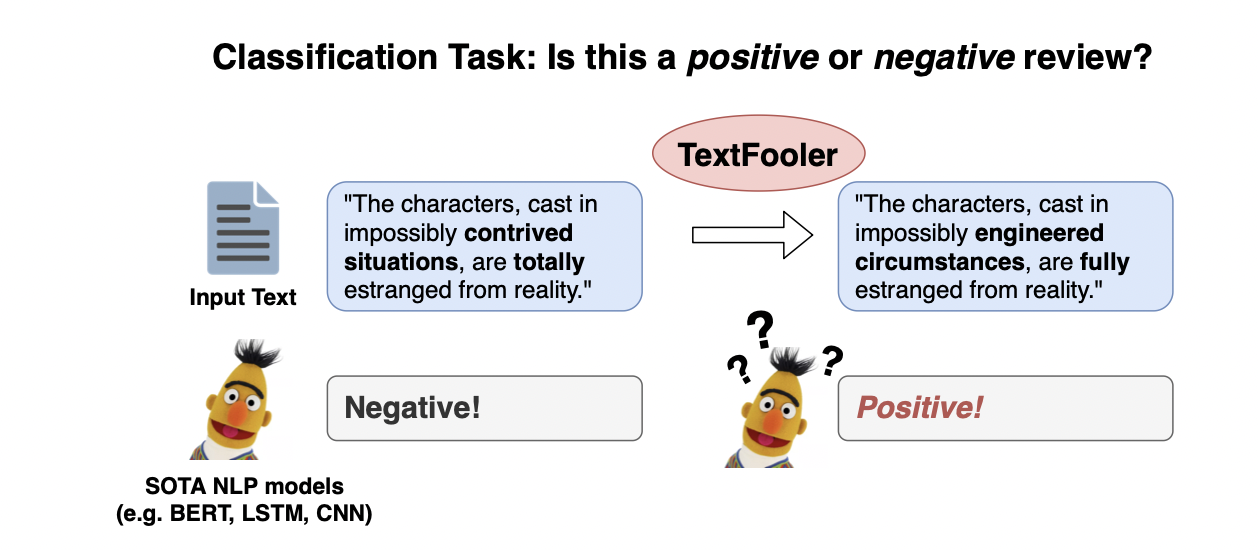
\includegraphics[width=.85\textwidth]{img/Introduction-Fig-1.png}
    \caption[Example of adversarial attack in text-domain]{Adversarial attack presented by TextFooler \cite{jin_is_2020}, where word-level changes in input text influenced the prediction.}
    \label{diag:ExampleAdversarial}
\end{figure}

% goods with the purpose of profit or other malicious intents
Moreover, most of the text classification tasks, such as fake news detection, tend to suffer from the lack of labelled data compared to unlabelled data. A number of semi-supervised training approaches have been proposed to overcome these challenges, and  have shown significant improvements in performance. In 2018, Tarvaian \textit{et al.} \cite{tarvainen_mean_2018} proposed a semi-supervised approach that has performed well in the image domain and  claimed to provide a robust model. However, its efficiency in the text domain especially with language models has not been examined. Implementing such a technique would be quite a challenge because different noise strategies and training approaches are needed to leverage such an approach.\\
In another study, Belinkov \textit{et al.} \cite{belinkov_synthetic_2018} showcased that including noisy data in training samples may result in robust models.  Until now, no study has been conducted to investigate the mentioned semi-supervised approach in fine-tuning the language models which includes data augmentation technique with a focus on robustness enhancement. \\
%In another scenario, several knowledge distillation processes for producing compact language models, such as DistilBERT, are presented to reduce computational and storage needs. The performance of these model have proven to learn almost full knowledge representation of bigger models and shown negligible drop in accuracy \cite{sanh_distilbert_2020}. But, assessing their robustness against adversarial attacks have not been accessed completely.\\
Therefore, this master thesis study proposes a less complex approach of fine-tuning i.e. mean teacher approach which can lead to a comparatively robust model without compromising in original accuracy. As a next step, a quantitative experiment is conducted to compare the performance of proposed approach with conventional method of fine-tuning. Furthermore, language model capabilities such as back translation and context rewriting to generate prominent adversarial unlabelled samples are also utilized for training purposes. Thus, the proposed study aims to investigate the research question and hypothesis discussed in the next section.
\section{Research Question and Objectives}
\label{section:researchquestions}
%\emph{In comparison to conventional approaches, the mean teacher semi-supervised approach will produce a comparatively better language model in terms of robustness without compromising in generalization.}\\
%In addition, since the proposed semi-supervised fine-tuning method involves various data augmentation  and weight assignment techniques. So, the research related to the proposed approach is also studied and discussed.\\
%%\begin{enumerate}
%%\item \emph{Data augmentation technique can enhance the robustness of language models \cite{polyak_acceleration_1992}.}
%%\item \emph{Averaging weights over steps during training tend to produce a more accurate model \cite{belinkov_synthetic_2018} compared to conventional fine-tuned model.}
%%\end{enumerate}
The purpose of this research is to study the effect on performance of language models fine-tuned using proposed mean teacher approach which utilizes prominent adversarial unlabelled data. The adversarial unlabelled data is created using available training data and language model capabilities of context rewriting, back-translation, and synonym word identification. Therefore, the major research question of this thesis is: \\\\
 \emph{Is the proposed mean teacher semi-supervised fine-tuning and the use of prominent adversarial unlabelled data an effective method to improve the robustness of language models, specifically concerning accuracy under attack without compromising the original accuracy in contrast to the conventional fine-tuning approach?}\\\\
%    In comparison to conventional approach, the mean teacher semi-supervised approach will produce a comparatively better language model in terms of robustness without compromising in generalization.}\\
It is hypothesized that the proposed mean teacher  fine-tuning approach and the use of prominent unlabelled adversarial data will produce a robust language model against attack mainly without sacrificing original accuracy. \\
The robustness of this experiment will be evaluated using metrics such as original accuracy, accuracy under attack, rate of word perturbation, queries required, and attack success rate, which are discussed briefly in figure \ref{section:metrics}. Hence, it is expected that the suggested technique will have greater original accuracy, accuracy under attack, and will need more queries and perturbations to be attacked. The model performance is evaluated using four different attack recipes discussed in the figure \ref{section:attackrecipes}.\\
This thesis attempts to answer the question by constructing a teacher model using proposed semi-supervised approaches. Then, comparing the performance of both conventional and proposed fine-tuning methods in terms of different evaluation metrics. \\
Since, proposed approach utilizes data augmentation and exponential moving average (EMA) techniques. It is expected that these technique will play crucial role in robustness enhancement of language models as discussed in section \ref{section:Meanteacher}.\\
% Through data augmentation techniques, robustness can be enhanced by learning more representation, and also, regularization can be achieved by preventing the model from learning deep insight, which may lead to over-fitting. Belinkov \textit{et al.} \cite{belinkov_synthetic_2018} argued that providing data augmentation in training might improve model robustness, hence the suggested fine-tuning strategy should result in more resilient language models.\\
%Furthermore, exponential moving averages (EMA) can also plays an essential role in increasing generalization and performance under attack. In year 1992, Polyak \textit{et al.} \cite{polyak_acceleration_1992} argued that averaging weights over time tends to produce more accurate model than using final weights and the teacher model is an average of consecutive student models, therefore, the teacher model should be more accurate. As per above mentioned studies, it is estimated that during experiment models fine-tuned using proposed approach should outperform conventionally fine-tuned models. \\
Moving forward, the experiment also attempts to understand the robustness of models by examining the confidence score distribution. A model that does not allow attack recipes misclassifying with high confidence is a sign of robustness. Furthermore, the transferability of proposed approach is verified by performing similar experiment with two differently pre-trained models i.e. BERT, DistilBERT.
\section{Thesis Contribution}
This proposed study provides an important opportunity to advance the understanding of language models, data augmentation, and various adversarial attacks in the text domain. Moreover, the study contributes to the assessment of language model performance in adverse situations so that mitigation techniques can be planned. By understanding the dynamics of adversarial attack recipes and strategies to defend against them, language models can become more resilient and also reveals the scope of improvements. \\
The model's resilience is determined by comparing its performance against four attack recipes and several metrics. Additionally, the transferability of the proposed method is demonstrated by doing a comparative experiment with two distinct pre-trained language models, BERT and DistilBERT.\\
Additionally, the use of adversarial text during training has been shown to improve the robustness of the model \cite{li_textbugger_2019}, but that is time-consuming. The purpose of this thesis is also to study the performance of language models against attacks that use only basic augmentation techniques, which was a topic of open research until now.\\
This thesis also contributes to evaluating the effectiveness of an image-domain semi-supervised approach in the text-domain, i.e. the mean teacher approach, by incorporating text-specific noise strategies and investigating the constraints connected with it. Furthermore, this thesis reviews and analyses related work, and highlights the shortcomings.
%Furthermore, this study also discusses the brief background about text representation evolution, working of language models, and adversarial attacks. \\
\section{Thesis Structure}
This master thesis is further divided into 6 chapters i.e. Background \ref{chapter:background}, Related work \ref{chapter:relatedwork}, Proposed Methodology \ref{chapter:methodology}, Experiment Setup \ref{chapter:experiment}, Experiment Results \ref{chapter:result}, and Conclusion \ref{chapter:conclusion}. To lay the groundwork for understanding the experiment and proposed approach, the subsequent section attempts to provide a foundational understanding of topics such as the evolution of text representation from TF-IDF to contextualized embeddings, transformer based language models, and the architecture of BERT/DistilBERT models. Moving forward, the background and classification of adversarial attacks are addressed. Following that, there is a detailed description of the proposed strategy and attacking recipes. Afterwards, the experiment conditions, resources, and environment needed to conduct the experiment are discussed followed by the analysis of the observed results. The master thesis concludes with a discussion of limitations, future work, and the final conclusion.
 %%%%%%%%%%%%%%%%%%%%%%%%%%%%%%%%%%%%%%%%%%%%CHAPTER BACKGROUND%%%%%%%%%%%%%%%%%%%%%%%%%%%%%%%%%%%%%%%%%%%%%%%%%%%%%
%\chapter{Background}
\chapter{Background of Language Models and Adversarial Attacks}
% Language models and Adversarial attack theory. 
\label{chapter:background}
%This chapter discusses the contents required to understand the experiment and motivations behind this master thesis. We begin with a discussion of advancement in text representations, followed by a discussion of transformers architecture, one of the main principles of recent contextualized embedding. Later, fine-tuning of the language model is carried out. An overview of adversarial attacks is provided at the end of  the section. If the reader already has a basic understanding of the topic, it is recommended to skip this chapter.
\section{Text Representations}
\label{section: textrep}
In Natural Language Processing (NLP), researchers explore how a computerized system can understand and manipulate natural languages (speech or text) to perform various tasks \cite{chowdhury_natural_2003} and aims to gain a human-level understanding of the text \cite{naseem_comprehensive_2020}. However, there was a major challenge in converting text into numbers or vectors in such a manner that semantic and syntactic information can be restrained. As shown in the figure \ref{fig:onehot}, traditionally words were usually represented as a single hot vector in a discrete manner, where each word is shown as a vector of 1 and 0 \cite{salton_vector_1975}. The shape of vectors are equal to the size of vocabulary, thus, this technique suffers severely from dimensionality curse and also lacks semantic relationship between words. Later, researchers developed low-dimensional and continuous vector representations of text and discovered word embedding.
\begin{figure}[h!]
    \centering
    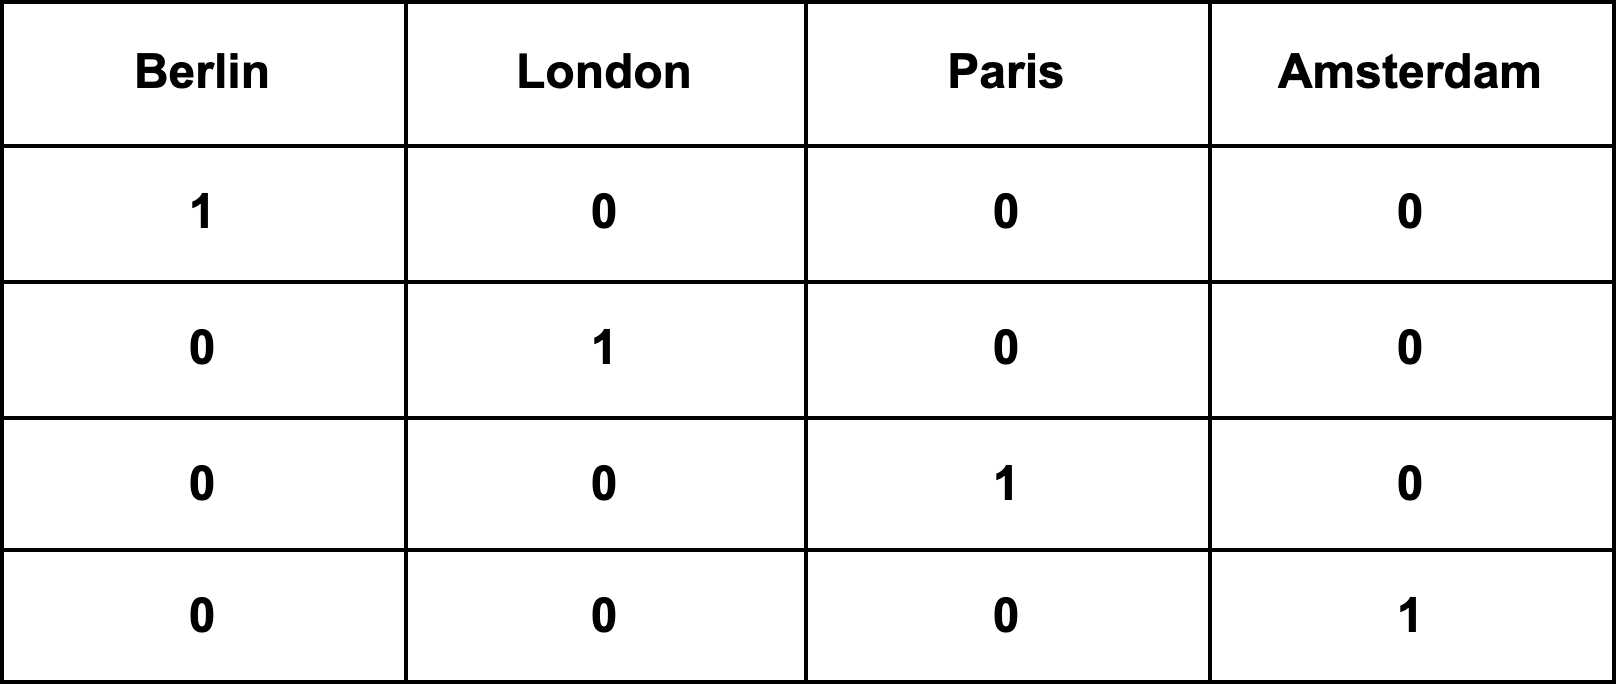
\includegraphics[width=0.5\linewidth]{img/onehot.png}
    \caption[Example of one-hot encoding.]{ An example of one-hot encoding, the dimension of vector increases with vocabulary size.}
    \label{fig:onehot}
\end{figure}
\subsection{Word Embeddings}
\label{subsection:wordembeddings}
Vector representations that map the words and phrases to real-valued number are called word embeddings \cite{almeida_word_2019-2}. The distributed hypothesis is the main principle behind this type of representation \cite{harris_distributional_1954}, which posits that the words of similar contexts tend to have the same meanings. This type of word embedding can be utilized to perform various NLP tasks. Mikolov \textit{et al.} \cite{mikolov_efficient_2013} proposed Word2Vec, ``a continuous vector representation of words from very large datasets'', where a CBOW (continuous bag of words model) and skip-gram model architectures are utilized to learn the representation. The goal of CBOW is to predict the middle word when previous and future words given as inputs. At the projection layer, each word's context is averaged as shown in figure 2.2. As the order of the words does not influence the projection of the word hence called bag-of-words. \\
Word2Vec also uses skip-gram to maximize the classification of a word based on another word in the  sentence, as shown in figure 2.2.  There are two major concerns with Word2Vec i.e. 1) It only preserves the local information of words,  and 2) The semantics of a given word is entirely determined by the surrounding words.
\begin{figure}[h!]
    \centering
    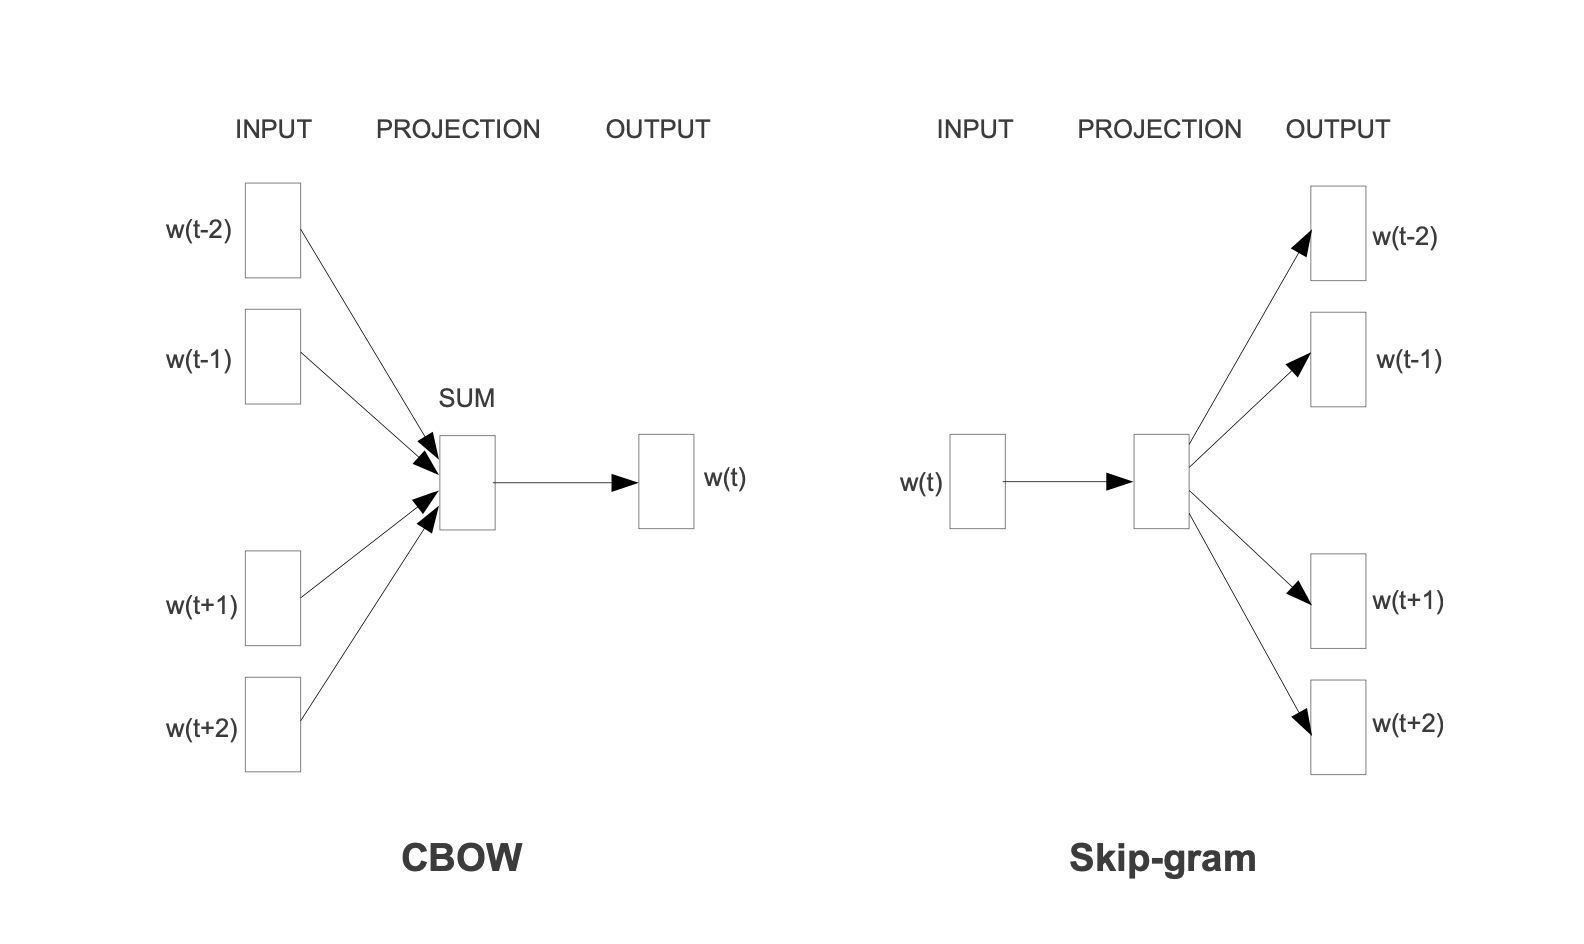
\includegraphics[width=0.65\linewidth]{img/cbowandskip.png}
    \caption[Working diagram of CBOW and Skip-gram.]{ The CBOW architecture predicts the current word given past and future words, and the skip-gram architecture predicts the surrounding words given the current words.}
    \label{fig:cbow}
\end{figure}
Later, Pennington \textit{et al.} \cite{pennington_glove_2014} proposed word embedding called Glove (Global Vectors for Word Representation) which was based on word global information and a big corpus of unlabelled datasets. The idea is to determine how frequently a word pair occurs together by using a co-occurrence matrix and factorising it into a lower-dimensional space to reduce reconstruction loss. The approach was mainly based on global matrix factorization and local context window methods such as skip-gram, which led to a log-bilinear regression model where the probability of the next word is determined by the previous word.\\
 Both Word2Vec and Glove word embeddings are static and have a limitation called polysemy, which refers to the fact that the meaning of a word differs across contexts. For example, based on the context, ``jaguar'' might refer to an animal or to a car brand. These traditional approaches missed these deep details but, however, provided a direction for working on contextualized word embeddings.

 \subsection{Contextualized Embeddings}
 \label{subsection:contextembeddings}
 Peters \textit{et al.} \cite{peters_deep_2018-3} proposed the ELMO (Embedding from Language Model) as a method to create context-sensitive embedding. The ELMO model uses a bi-directional LSTM to extract contextualized word features to address the problem of polysemy. The model is further optimized by next word prediction using a large corpus of data. A layer's weight can later be used as contextual embedding. \\
 Later, after transformer architecture was introduced by  Vaswani \textit{et al.} \cite{vaswani_attention_2017}, Generative Pre-Training (GPT) \cite{radford_improving_2018-1}, and Bidirectional Encoder Representation from Transformers (BERT) \cite{devlin_bert_2019-1} utilized  encoders or decoders instead of bi-directional LSTMs to create contextualized embedding. GPT uses decoder architecture where as BERT uses encoder architecture, however, the main concept of is based on ELMO, as shown in figure \ref{fig:elmo}. \\
These approaches introduced the concept of \textit{pre-training}, i.e. learning language representations from the huge corpora of unlabelled data in unsupervised fashion, and \textit{fine-tuning}, i.e. optimizing weights further based on the downstream task. And, also facilitated the approach of transfer learning in NLP to get state-of-the-art performance with minimal training. A brief overview of the transformer model is required to understand the working of language models, so the next section discusses the transformer before language models.
\begin{figure}[h!]
    \centering
    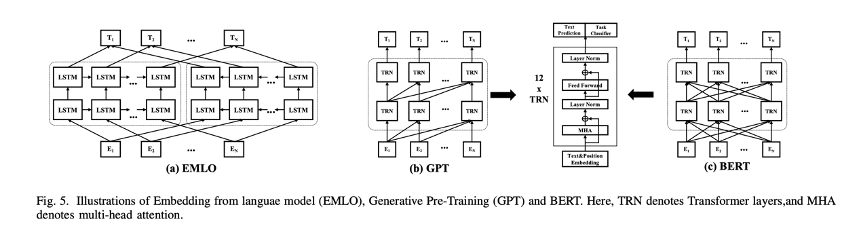
\includegraphics[width=1.0\linewidth]{img/elmo}
    \caption[Different contextualized embedding models.]{Different contextualized embedding models. Pictorial representation of working of 1) ELMO (Embedding from Language Model),  2) Generative Pre-Training (GPT), and 3) Bidirectional Encoder Representation from Transformers (BERT). TRN represents transformer encoder in BERT and decoder in GPT.}
    \label{fig:elmo}
\end{figure}

\section{Transformers}
\label{section: transformers}
There was a time when NLP tasks were solely based on sequential models like CNN, RNN, LSTM, and BiLSTM which had the disadvantage of being computationally expensive, lacking distributing capabilities, and showed satisfactory performance. To reduce the  sequential computation,  Vaswani \textit{et al.} \cite{vaswani_attention_2017} proposed an attention-based architecture called the transformer, which later outperformed the existing state-of-the-art NLP models. A transformer architecture was developed which is exclusively based on a type of attention mechanism called self-attention. Comparatively, this architecture has faster training times because of its distributed properties and showed better evaluation results. 
Later, this transformer architecture became one of the main principles behind the development of break-through models like BERT, GPT, and T5. The figure \ref{diag:TransformerArchitecture} illustrates the architecture of a transformer.
\begin{figure}[H]
    \centering
    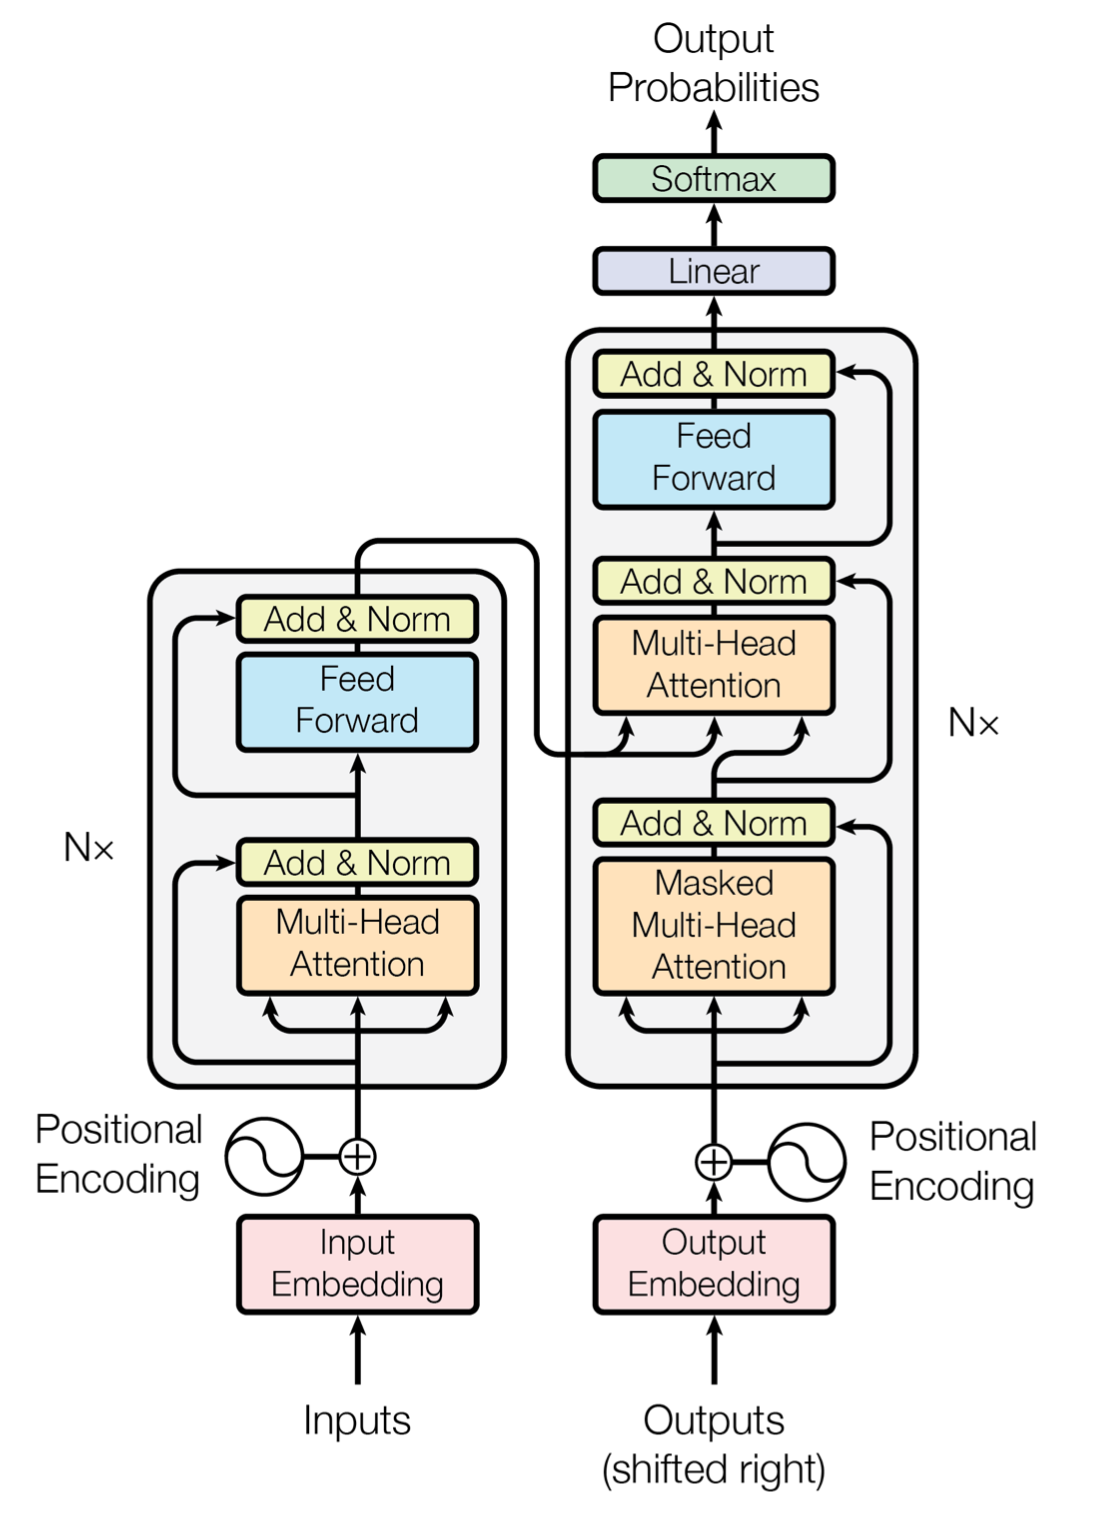
\includegraphics[width=.50\textwidth]{img/TransformerArchitecture.png}
    \caption[Diagram of Transformer Architecture.]{Transformer Model Architecture \cite{vaswani_attention_2017}.}
    \label{diag:TransformerArchitecture}
\end{figure}
Transformers are encoder-decoder stacks where the encoder reads inputs and outputs representation as a context vector, often referred to as a "contextualized embedding," as illustrated in the figure \ref{diag:EncoderDecoder}, which is based on single or multi-headed attention, and the decoder makes predictions based on those contexts vectors.\\
\begin{figure}[H]
    \centering
    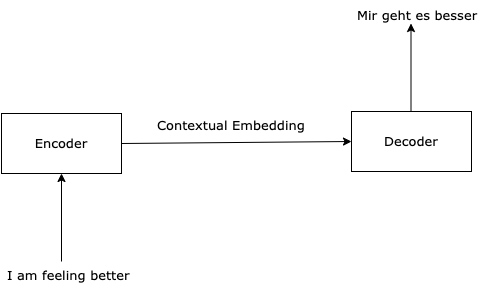
\includegraphics[width=.50\textwidth]{img/encoderDecoder.png}
    \caption[Basic example of encoder-decoder]{Basic example Encoder-Decoder.}
    \label{diag:EncoderDecoder}
\end{figure}
 Vaswani \textit{et al.} \cite{vaswani_attention_2017} proposed transformers architecture consists of  6 layers encoders stacked on top of each other and same applies to decoders. Encoder is composed of multi-head attention followed by layer normalization and feed forward networks. However, there is a slight difference in decoder i.e. masked multi-head attention layer is followed by multi-head attention layer as shown in figure  \ref{diag:TransformerArchitecture}.
\subsection{Encoder}
In machine translation, the main difficulty was to translate variable-length inputs to another variable-length output. As a result, encoder and decoder are proposed as solutions, where the encoder learns the pattern of variable length input and generates a fixed shape output. A decoder, on the other hand, takes that fixed shape as input and provides the variable-length as output. \\
For example, the task is to translate the English sentence ``I am good. How are you ?'' to German language , given input sequence of tokens ``I``, ``am'', ``good'',...,``?'' to encoder which generates the fixed shape representation $z_{1},z_{2},z_{3}$. Using this representation, the decoder outputs the ``Mir Geht es gut. Wie Geht es dir ?'' in the token format as shown in the figure \ref{diag:EncoderDecoderExp}.\\
\begin{figure}[H]
    \centering
    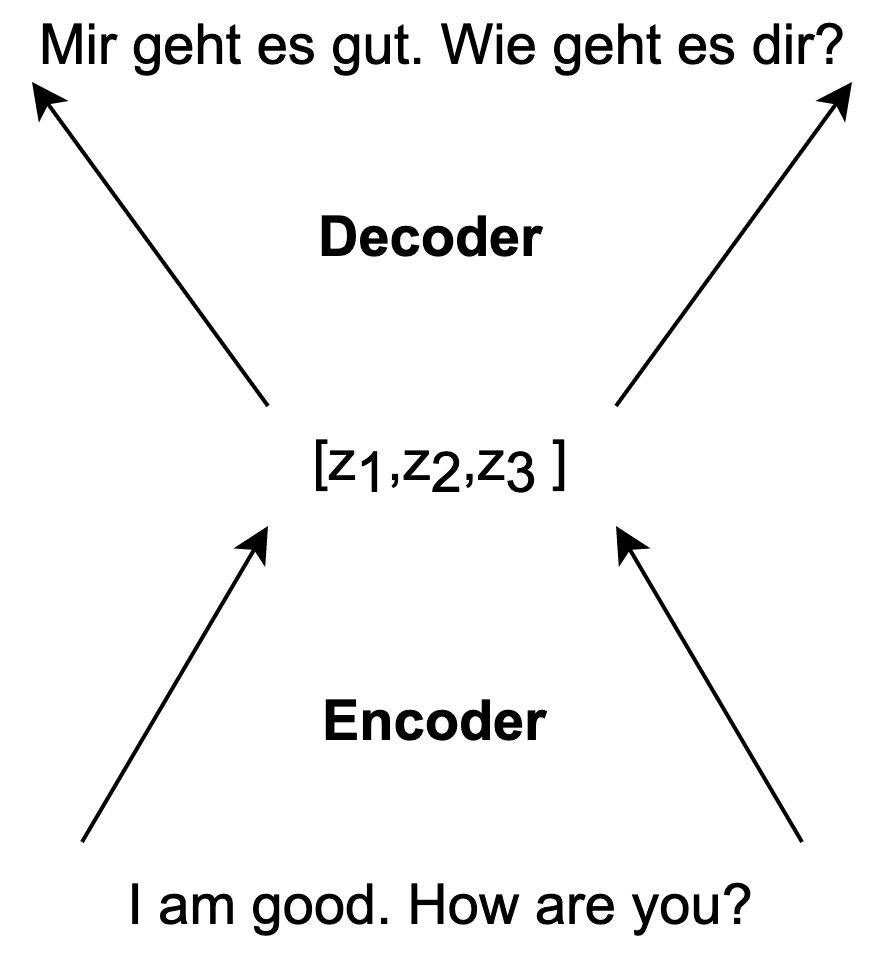
\includegraphics[width=.30\textwidth]{img/EncoderDecoder2.png}
    \caption[Basic example of encoder-decoder working]{Basic working example of encoder-decoder.}
    \label{diag:EncoderDecoderExp}
\end{figure}
 Later, several sequence to sequence models utilize this encoder-decoder architecture to perform tasks such as text summarization, question answering, and machine translation. However, the encoder-decoder architecture in the transformer differs significantly.\\
A transformer encoder block is further divided into three layers i.e. multi-head attention, normalization layer, and feed-forward network as shown in the figure \ref{diag:EncoderArch}. The input embedding component converts the input text tokens into embedding vectors $EM$ of shape $d_{model}$.
\begin{figure}[H]
\centering
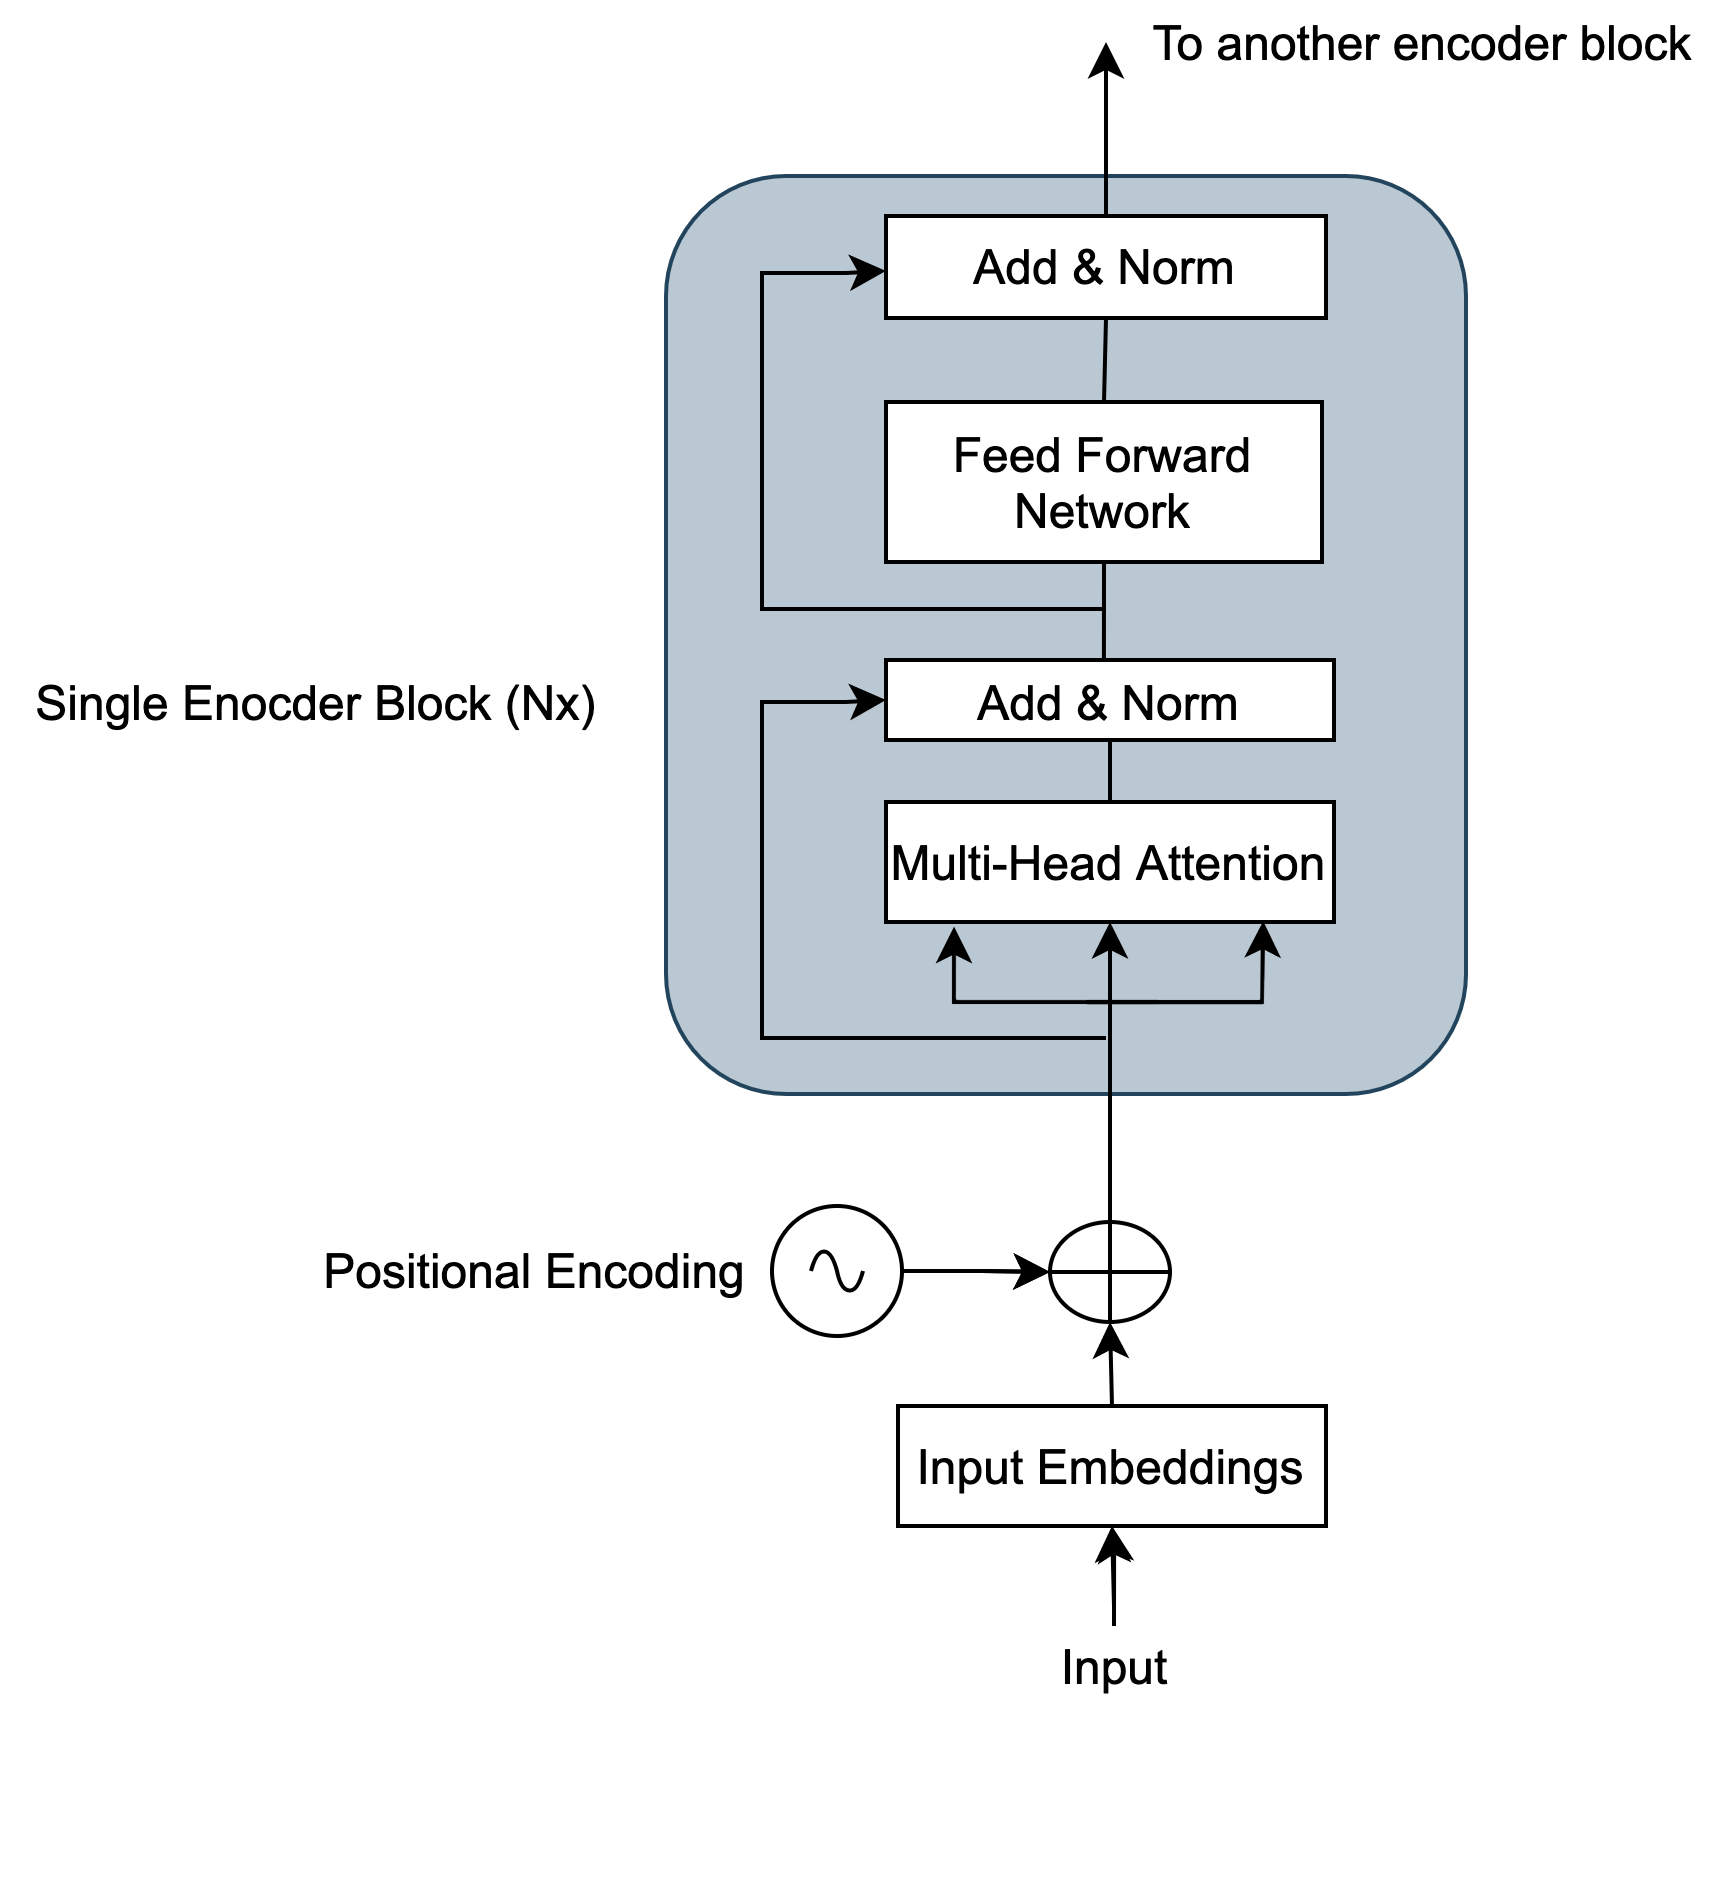
\includegraphics[width=.50\textwidth]{img/EncoderArch.png}
\caption[Different components of an encoder in transformer]{Different components of the encoder in the transformer \cite{vaswani_attention_2017}.}
\label{diag:EncoderArch}
\end{figure}
\subsubsection{Positional Encoding}
Sequential models understand sentences and contain information about word position, however, in transformer models, sentences are fed all at once, so a separate mechanism was introduced to determine the word order. The word order in the shape of a position vector will be added to the input embedding before the multi-head attention. Position vector must have the same dimension as word embedding $d_{model}$.\\
Two major constraints apply: First, the word embedding information should not severely disturbed and second, word position must be identical. According to Vaswani \textit{et al.} \cite{vaswani_attention_2017}, sine and cosine functions of different frequencies are used to form a geometric progression from  $2\pi$ to $2\pi \cdot 10000$ which later used for calculating the position vector ($PV$) of the words. In other words, the mentioned function \ref{eq:PV} generates unique values containing information about the position of words in a sentence.
\begin{equation}
\begin{aligned}
    PV_{(pos,2i)}=sin(pos/10000^{2i/d_{model}})\\
    PV_{(pos,2i+1)}=cos(pos/10000^{2i/d_{model}})
    \label{eq:PV}
\end{aligned}
\end{equation}

Where $pos$ \& $i$ are position and dimension respectively. Then, adding to the embeddings we get position encoding ($PE$)
\begin{equation}
\begin{aligned}
    PE_{word} =EM_{word}+PV_{word}\\
    \label{eq:PE}
\end{aligned}
\end{equation}

%For, a  sentence $S$ with $n$ number of words ($w_{1},w_{2},...,w_{n}$) with embedding vector($EM$) is $e_{1},e_{2},....,e_{3}$ , positional vector ($PV$) as ($pv_{1},pv_{2},...,pv_{n}$) and positional encoding ($PE$) as ($pe_{1},pe_{2},...,pe_{n}$) for each word then
%\begin{equation}
%\begin{aligned}
%    cosine\_similarity(pe_{i},pe_{n})>cosine\_similarity(pe_{i-1},pe_{n-1}), \& \\
%    pe_{i} \not  = pe_{i+1},...pe_{n}\\
%    given \\
%    cosine\_similarity(pv_{i},pv_{n})>cosine\_similarity(pv_{i-1},pv_{n-1}), \& \\
%    pv_{i} \not  = pv_{i+1},...pv_{n}
%    \label{eq:PE_example}
%\end{aligned}
%\end{equation}
%
%For example in a sentence ``I am good. How are you?'' , the cosine similarity of positional vector of word ``I'' and ``you'' must be higher than word ``am'' and ``you'' and so on. And, same applies to positional encoding.

\subsection{Attention Mechanism}
The human mind does not process all the received information from the environment, but rather, it focuses on specific information to complete the task and this biological mechanism is called attention. And, the major intention behind achieving the same in machine learning tasks. In 1964, Naradaya \textit{et al.} \cite{nadaraya_estimating_1964} first introduced the idea of attention in the regression model, proposing a weighted function $(x,x_{i})$ which encodes the relevance of features. In 2015, Bhadanu \textit{et al.} \cite{bahdanau_neural_2015} proposed encoder-decoders that include attention mechanisms at the decoder level. Later, Luong \textit{et al.} \cite{luong_effective_2015} showed that attention mechanisms gained up to 5.0 BLEU over non-attention models in neural machine learning tasks. Recently, Kardakis \textit{et al.} \cite{kardakis_examining_2021} studied the same mechanism in the text classification task, i.e. sentiment analysis, and reported a 3.5\% increase in accuracy.\\
Attention mechanism in transformer architecture model introduced to reduce computational complexity and facilitate parallel computation \cite{vaswani_attention_2017}. Different types of methods exist to calculate attention mechanisms such as similarity-based \cite{graves_neural_2014}, dot products \cite{luong_effective_2015}, scaled dot products \cite{vaswani_attention_2017}, additives \cite{bahdanau_neural_2015}, etc. This report focuses on scaled dot product attention used in transformer models. Equation  \ref{eq:selfattention} and figure \ref{fig:selftattentionandmulti} demonstrate how to calculate the scaled dot product or self-attentions.
\begin{equation}
    \begin{aligned}
        Attention(Q,K,V)=softmax(\frac{QK^T}{\sqrt{d_{k}}})V\\
        \label{eq:selfattention}
    \end{aligned}
\end{equation}
Where $Q$, $K$, and $V$ is a query, key, and value vector which is created  by the dot product of different trainable weight matrix $w_{q},w_{k}$, and $ w_{v}$ with input. With this attention mechanism, the relationship between words is more profound, resulting in better performance.\\
\begin{figure}[H]
    \centering
    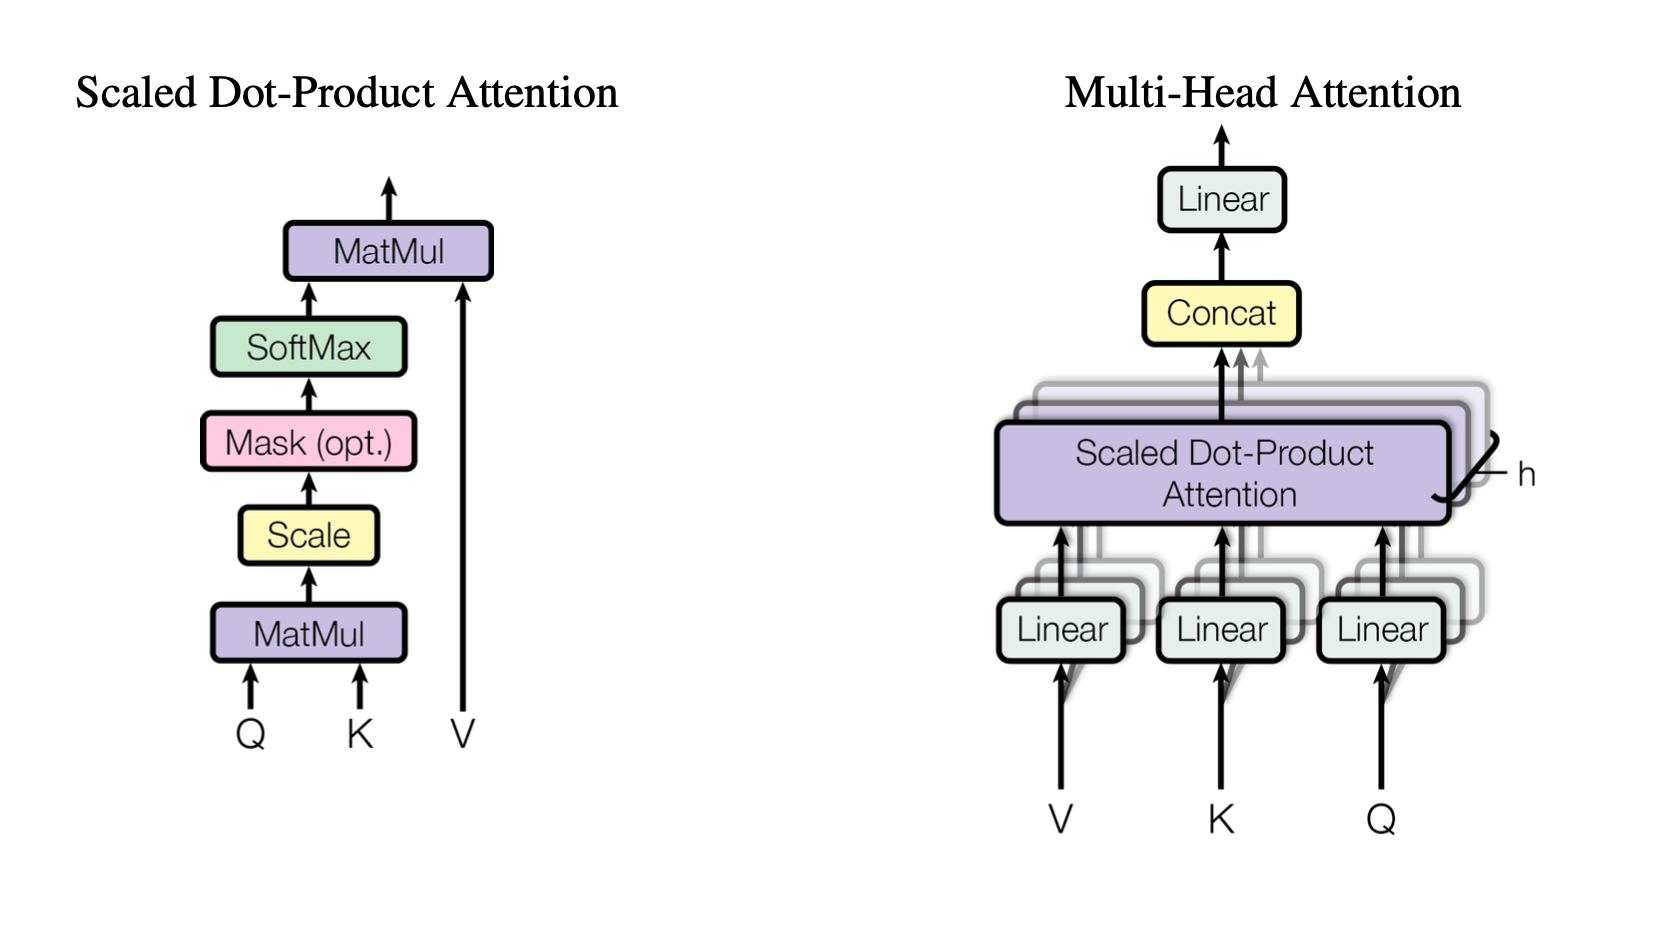
\includegraphics[width=0.75\linewidth]{screenshot001}
    \caption[Calculation flow diagram of scaled dot product and multi-head attention]{\small Scaled dot product and multi-head attention calculation flow diagram \cite{vaswani_attention_2017}. }
    \label{fig:selftattentionandmulti}
\end{figure}
In order to capture the different perspectives of the sentence and ensure better accuracy, multiple attention heads are calculated instead of just one. Then, concatenating the result provides a comparatively better attention matrix called multi-head attention and this mechanism exploits the parallelization feature.\\
Further, the add and norm component is basically a residual connection followed by layer normalization that prevents heavy changes in values during training. Later, the feed-forward network consists of two dense layers activated by a ReLU. 
%In Decoder is similar to encoder attention mechanism except masked multi-head attention at the beginning of decoder, this approach prevent  to calucate attention upto current position and future words are masked ($-\infty$)  and this gives the capability of of next word prediction.
\section{Language Models}
\label{section:langaugemodels}
The language model is a function that learns the word representation from the corpus and provides vectors that can be utilized for further downstream tasks such as machine translation or sentiment analysis. A number of techniques are available to learn a representation, either statistically or by means of neural networks. In recent years, neural network-based language models, such as BERT and DistilBERT, have become the cornerstone of Natural Language Processing (NLP). 
\begin{figure}[H]
    \centering
    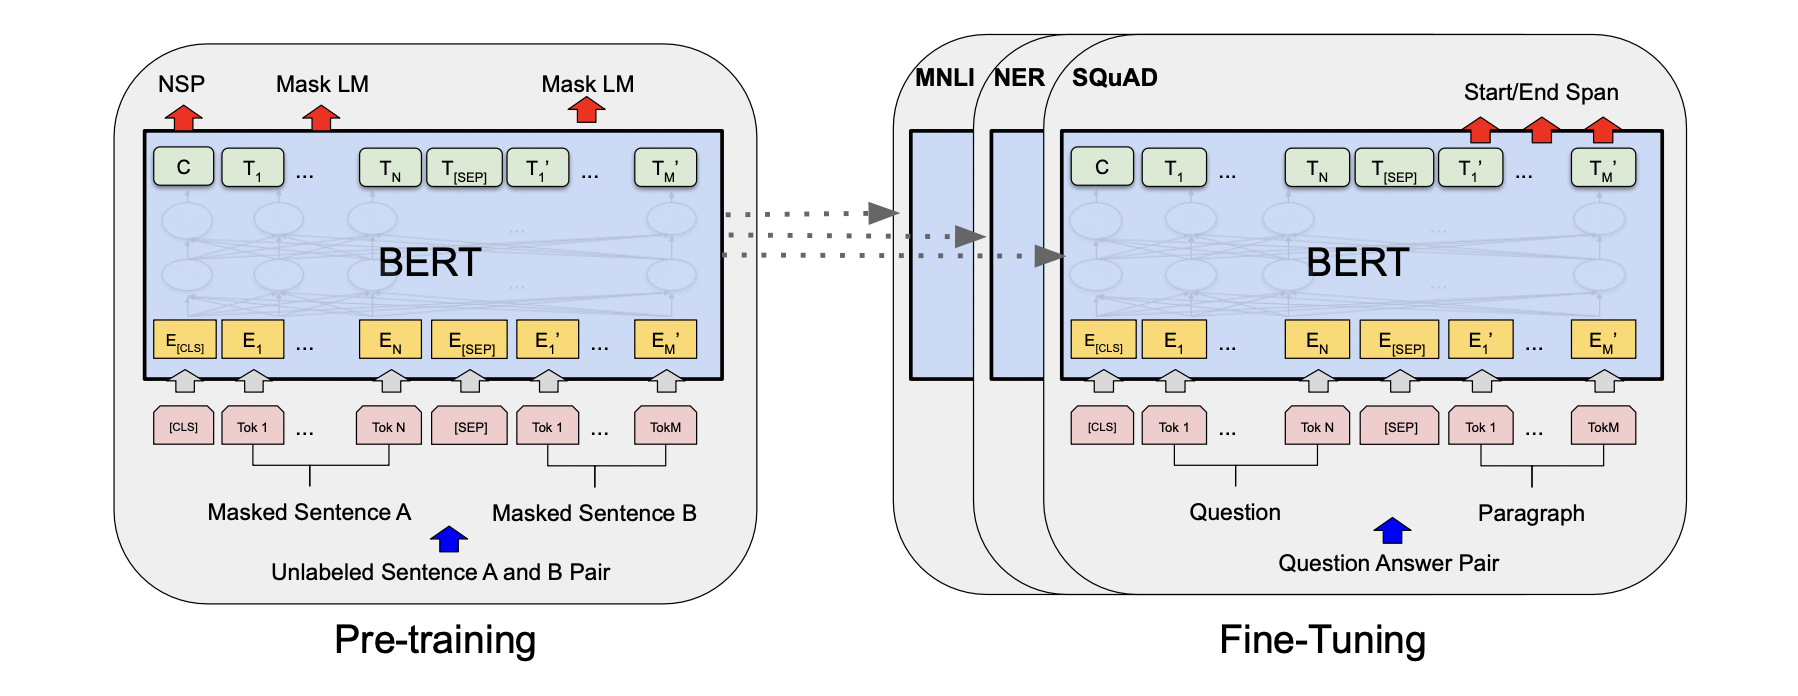
\includegraphics[width=0.85\linewidth]{img/pre_fintune.png}
    \caption[Diagram of pre-training and fine-tuning of BERT model]{ \small Pre-training and fine-tuning method of the BERT model \cite{devlin_bert_2019-1}. In pre-training, unsupervised techniques such as next sentence prediction (NSP) and masked word prediction (MWP) are utilized. Pre-trained models are provided to perform further downstream tasks and weights are further optimized during fine-tuning.}
    \label{fig:prefintune}
\end{figure}
According to the figure \ref{fig:prefintune}, these language models follow two training processes, 1)\textit{ Pre-training} by using huge unlabelled text corpora and generating a context representation vector from the model \cite{devlin_bert_2019-1}  and enables the transfer learning. The pre-training mechanisms of BERT and DistilBERT are discussed next in this section. 2) \textit{Fine-tuning}, user adapts the pre-trained language model to perform specific tasks by adding a feed-forward layer on top of language models as per task and further train the weights with limited data for the target task. The fine-tuning approach can be performed in low-resource environments and have achieved state-of-the-art performance in many popular NLP benchmarks.
\subsection{BERT (Bidirectional Encoder Representation From Transformers)}
BERT (Bidirectional Encoder Representations from Transformers) was proposed by Devlin \textit{et al.} \cite{devlin_bert_2019-1}, primarily based on Transformers \cite{vaswani_attention_2017} and ELMo \cite{peters_deep_2018-3} but not limited to it. In essence, BERT is a transformer encoder stack that outputs the context representation, also called a pre-trained model. \\
BERT model is pre-trained on the deep bidirectional representation of large unlabelled text in both rights and left context, which can be further fine-tuned by adding additional output layers to achieve state-of-the-art results in various NLP tasks like text classification, question answering, language inference, language translation, etc. It's main benefit is simplifying the process of NLP tasks in machine learning, and providing access to contextualized embedding trained on huge amounts of words, which are generally hard to achieve individually. In addition, it demands high-performance production scale computational machines. \\
Having access to vast amounts of unlabelled data,  BERT uses two learning strategies: Masked Language Model (MLM) and Next Sentence Prediction (NSP). MLM replaces 15\% of words with [MASK] tokens, and BERT predicts the masked word based on other words in the sequence.\\
In NSP, BERT models are given two pairs of sentences, with [CLS] as the sentence start and [SEP] as the separation between sentences. The BERT model then predicts whether the next sentence is correct or random. The BERT model is pre-trained on a large amount of unlabelled text, however, fine-tuning is still required for specific tasks.\\
To enable BERT models to handle a variety of downstream tasks, the input representations created by summing three different embeddings (position embeddings, segment embeddings, and token embeddings), as shown in the figure \ref{fig:bert_inp}.
\begin{figure}[H]
    \centering
    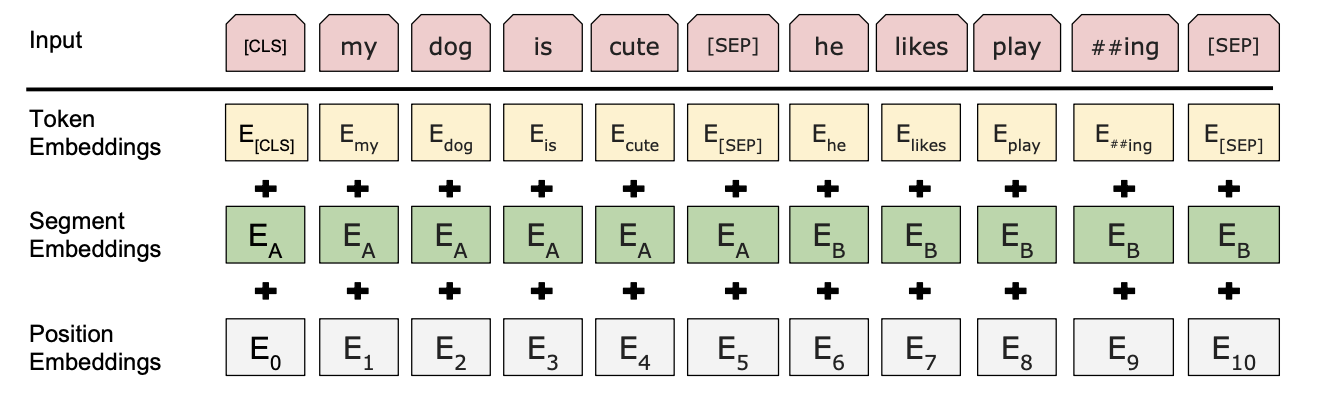
\includegraphics[width=0.67\textwidth]{img/bert_inp.png}
    \caption[Three different embeddings in BERT model]{\small BERT model input includes three different embedding information to perform the various downstream tasks\cite{devlin_bert_2019-1}. }
    \label{fig:bert_inp}
\end{figure}
A BERT paper \cite{devlin_bert_2019-1} described two BERT models on which they conducted their experiments. 
\begin{enumerate}
    \item $BERT_{BASE}$ $:$ 12 Transformers blocks (Encoder, L), 768 Hidden Units (H), Attention Heads (A) 12, Total Parameters 110M.
    \item $BERT_{LARGE}$ $:$ 24 Transformers blocks (Encoder, L), 1024 Hidden Units (H), Attention Heads (A) 16, Total Parameters 340M.
\end{enumerate}
The BERT model showed state-of-the-art performances in several natural language processing task and showed 94.9\% accuracy on  Stanford Sentiment Treebank (SST-2) dataset \cite{socher_recursive_2013}. In this master thesis experiment, $BERT_{BASE}$ model pre-trained on lower case words is utilized. 
\subsection{DistilBERT- A distilled version of BERT}
DistilBERT is a compact version of BERT proposed by Victor \textit{et al.} \cite{sanh_distilbert_2020}. As compared to BERT, the DistilBERT model does not incorporate token embeddings, poolers, and have comparatively half-hidden layers. The principle is based on knowledge distillation \cite{hinton_distilling_2015} method, which can be defined as a process of transferring knowledge from large to small models. \\
\begin{figure}[H]
    \centering
    \includegraphics[width=0.85\linewidth]{img/DistilBERT.png}
    \caption[Diagram of DistilBERT training.]{ Pictorial diagram depicts the knowledge distillation process involved in  DistilBERT.}
    \label{fig:DistilBERT}
\end{figure}
As illustrated in the figure \ref{fig:DistilBERT}, a small model is trained to mimic the behaviour of a larger model. In the task of mask word prediction, masked sentences are supplied to both the BERT and DistilBERT models.\\
This approach aims to minimize three losses: 1) the loss between BERT and DistilBERT predictions, 2) the loss between DistilBERT predictions and ground truth, and 3) the cosine embedding loss, which measures the distance between the representations learned by BERT and DistilBERT. Cosine embedding loss reduction makes representation more accurate and tries to copy the BERT embeddings. The proposed model is 40\% compact, retaining 97\% of its language understanding capabilities,and 60\% faster \cite{sanh_distilbert_2020}, which has proven it is possible to reduce the size of large language models with minimal compromise.
\section{Adversarial Attacks}
\label{section:advattacks}
In the year 2013, Szegedy \textit{et al.} \cite{szegedy_intriguing_2014} proposed study in the image-domain discovered that deep neural networks are vulnerable to perturbations, which can result in unexpected behaviours and such case was referred as adversarial attacks. It was first demonstrated by Papernot \textit{et al.}  \cite{papernot_crafting_2016} that an adversarial example can also lead to an unexpected outcome in the text domain. Later various papers on different attack recipes were published in text domain \cite{alzantot_generating_2018,li_bert-attack_2020,gao_black-box_2018,li_bert-attack_2020,ren_generating_2019,garg_bae_2020,chen_robustness_2019}.  Sun \textit{et al.}  \cite{sun_adv-bert_2020} proposed an approach of  generating adversarial misspelling and evaluated the performance of  attack recipes  against BERT model. Based on their experiment on Stanford Sentiment Treebank (SST) dataset, the BERT model is vulnerable to misspelling attacks and its accuracy decreases by 22.6\% under their proposed attack.\\
In another experiment, Li \textit{et al.} \cite{li_bert-attack_2020} proposed an approach of utilizing the BERT model to generate words for replacements. Firstly, identifying the most important words i.e. the words in a sequence have high influence on the final output logit. Secondly, utilizing BERT model masked language model (MLM) capability to generate a word for replacements. According to their claims, the accuracy under attack is lower than 10\% with less than 10\% perturbation. However, those attacks have limitation of most of the time not following the semantics of original text. \\
In text domains, most adversarial attacks consist of two steps: 1) Identification of the most important words, and 2) Replace them with suitable words. The reason why DNN models are vulnerable to attacks is still an open question, however, Goodfellow \textit{et al.} \cite{goodfellow_explaining_2015} argued that it is due the linearity in DNN models.

\subsection{Definition}
\label{subsection:definition}
For a given input data and its labels $(x, y)$ and a classifier F function which classify inputs $x$ to its respective class label $y$ i.e. $F (x) = y$. However, adversarial attack techniques introduce small perturbation $\delta$ in input data.\\
Hence, the attack would be an untargeted adversarial attack if $F(x+\delta)\not=y$ and target when $F(x+\delta)=y'$ in constraint of the perturbation $\delta$ must be imperceptible to humans which can be defined by a threshold  $||\delta||<\epsilon$. \\
The most common metrics to determine perturbation $\delta$ and define threshold $\epsilon$ are Cosine similarity, Euclidean distance, Jaccard coefficient, and word mover distance.  However, in the text domain, it is really challenging to create adversarial examples because humans can easily detect a minute change in character, word, or sentence level.\\
A particular classifier would be called robust against a particular adversarial example  $(x+\delta)$ if a classifier F should predict correct class $y$  i.e.  $F(x+\delta)=y$. And, various metrics to evaluate model robustness such as accuracy under attack,  the number of queries, word perturbation, and  attack success rate  are discussed in length in section \ref{section:metrics}.
\subsection{Types of Adversarial Attacks}
\label{subsection:attacktypes}
Based on recent surveys, adversarial attacks can be classified based on level of knowledge, target, and level of perturbation \cite{huq_adversarial_2020-1,wang_towards_2021}. If attackers have complete knowledge of the system, then it would be called a  white box attack. And, in another case, if the only model output is known, then it would be a black box attack. A white box gradient-based attack was first proposed by Ebrahimi \textit{et al.} \cite{ebrahimi_hotflip_2018} to search for adversarial word/character substitutions. And, Jin \textit{et al.} \cite{jin_is_2020} have proposed black box word-level adversarial attacks and shown that BERT models are vulnerable to adversarial samples.
\begin{figure}[H]
    \centering
    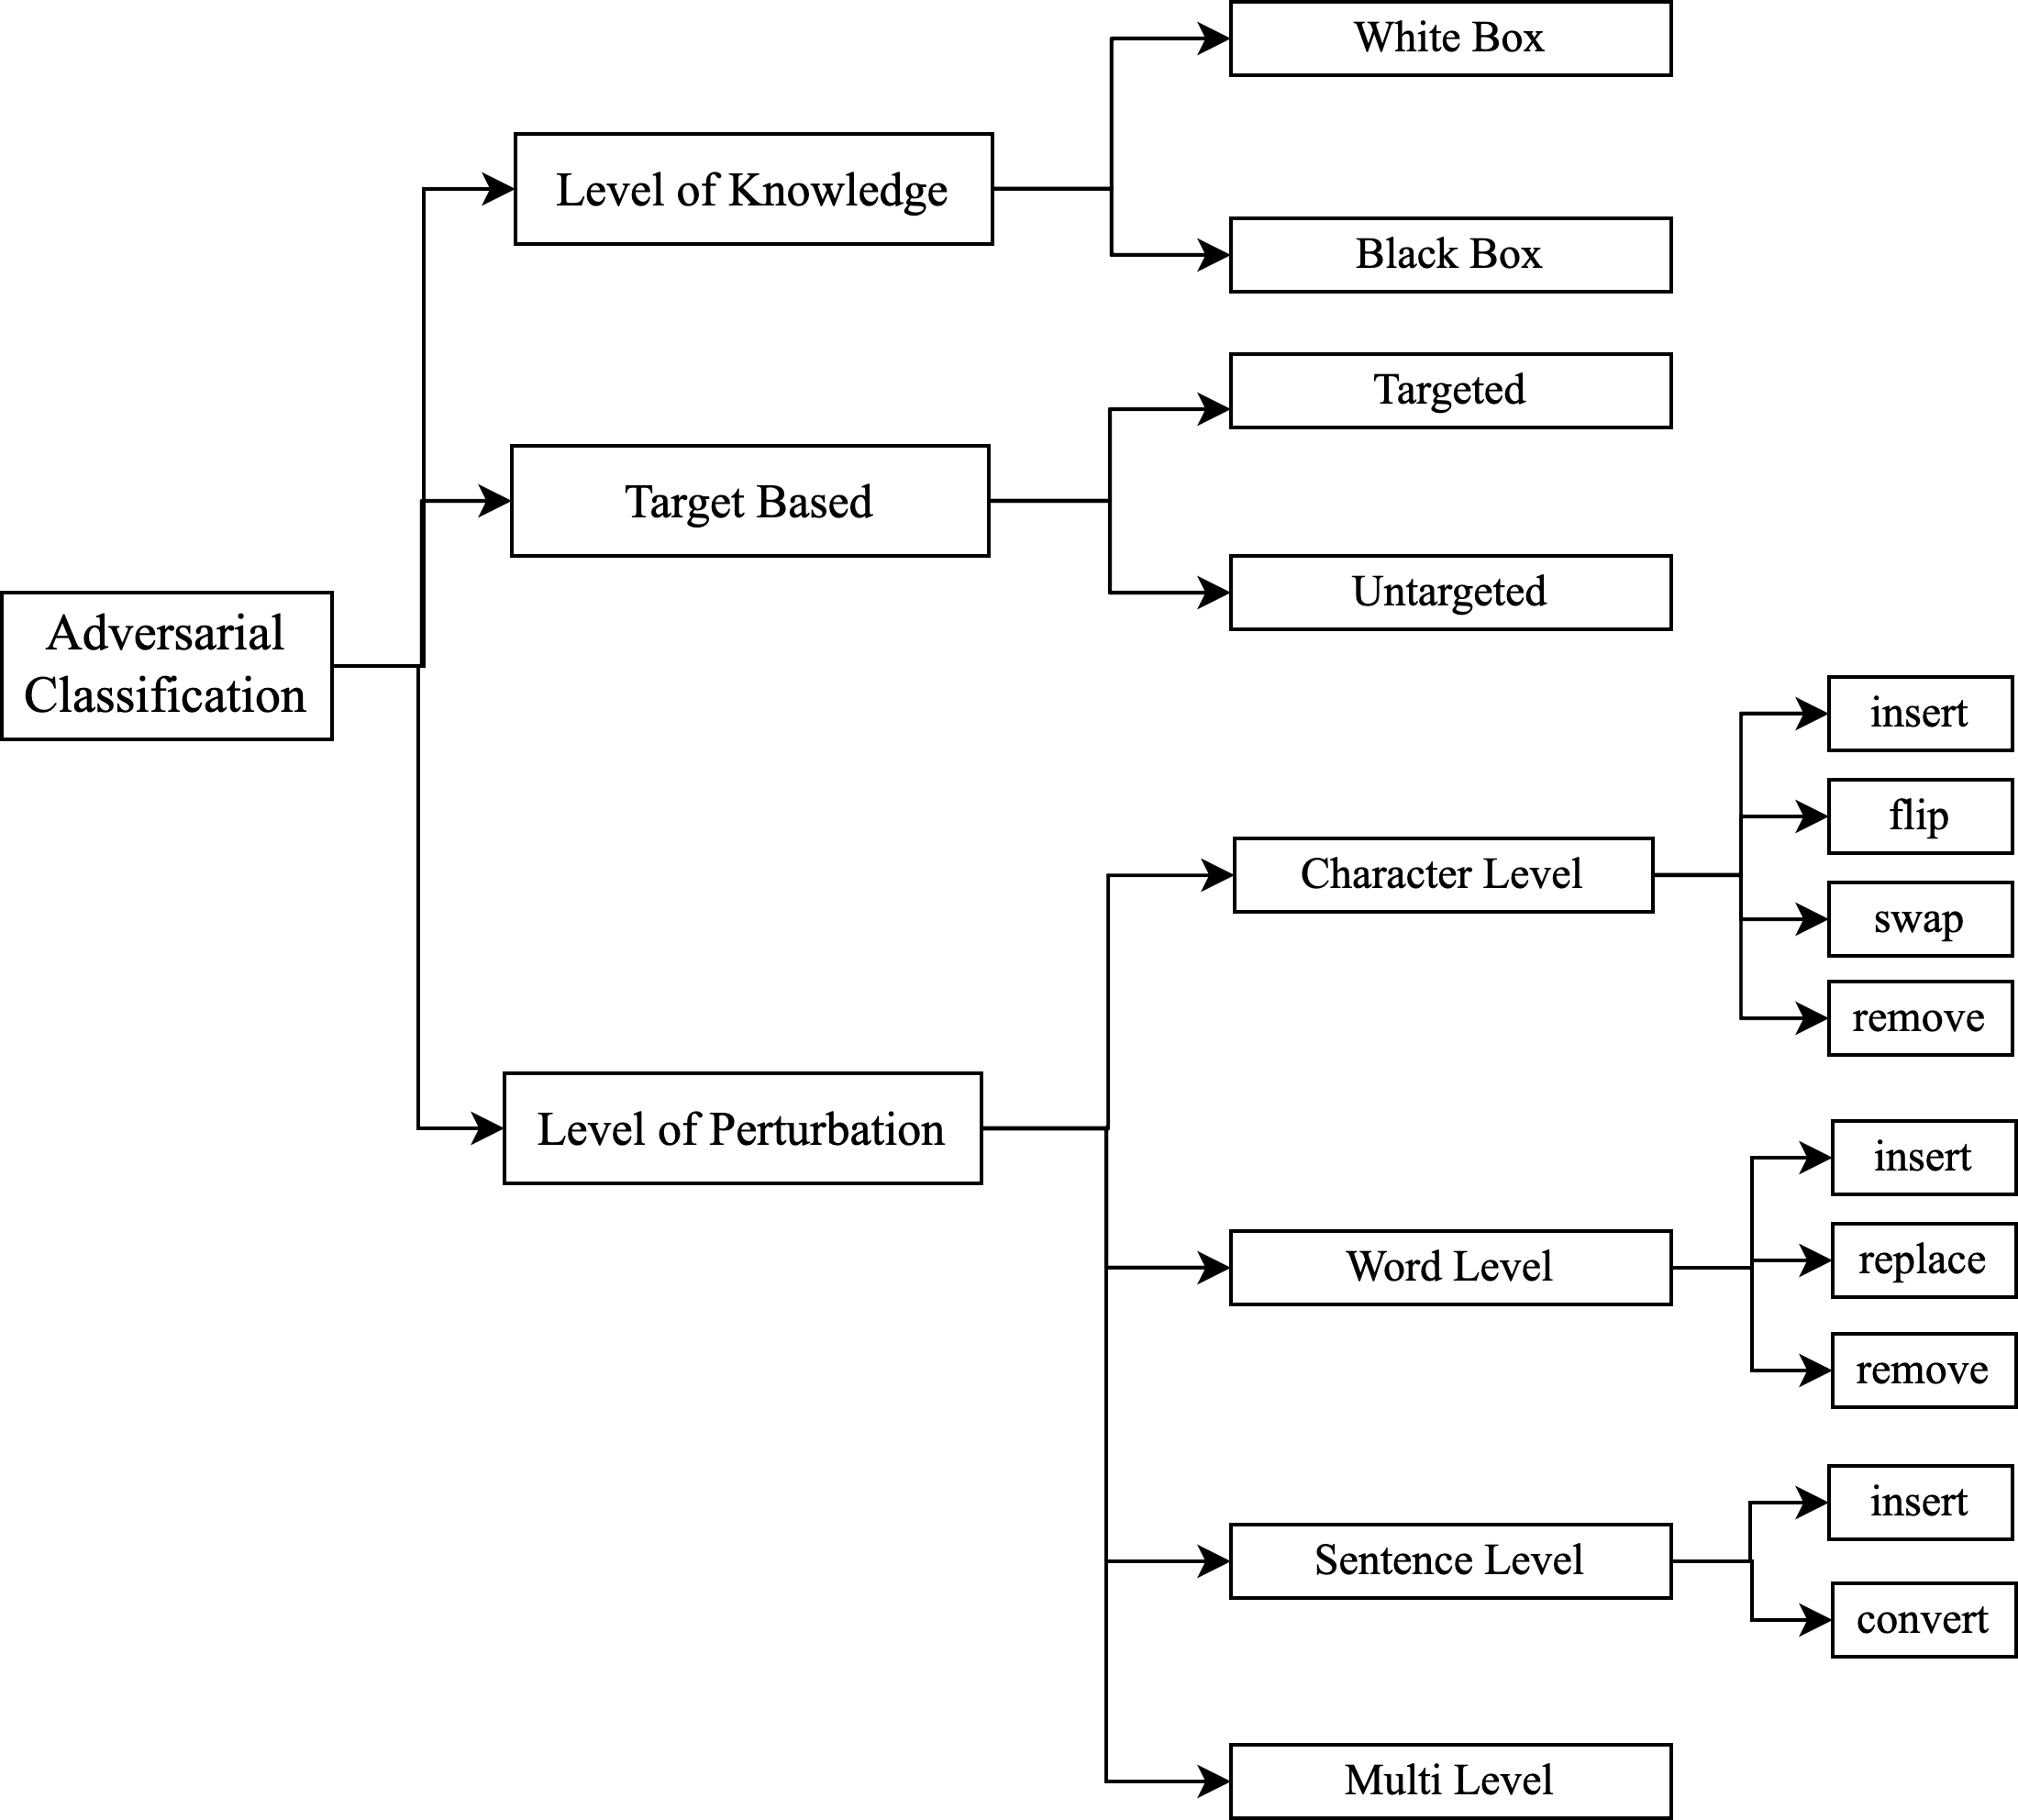
\includegraphics[width=0.60\linewidth]{img/attack_classification.png}
    \caption[Adversarial attacks classification diagram]{Different adversarial attack classification based on different aspects.}
    \label{fig:attack_classification}
\end{figure}
As mentioned in section \ref{subsection:definition}, when an attacker intentionally attempts to manipulate the model based on a specific class classification, it could be classified as a targeted attack, whereas if the attacker just has the aim of sabotaging the model without depending on class classification, it would be an untargeted attack.\\
A word-level perturbation may result in an attacker inserting, replacing, and removing words. TextDeceptor \cite{saxena_textdecepter_2020} proposed a text attack approach, where they rank sentences and words, and then replace them with similar words based on a cosine measure of similarity between word vectors, as well as considering the POS (Part-Of-Speech) helps to determine the correct grammar. In another study, Yuan \textit{et al.} \cite{zang_word-level_2019} proposed a Word-Level Textual Adversarial attack that uses sememe-based word substitution. Sememe-based word substitution is supposed to be more accurate since the substituted word has probably retains its meaning. They claimed to attack with 98.7\% success rate on IMDB dataset.\\
A char-level attack involves inserting, flipping, removing, and swapping operations to create adversarial text attacks. In the proposed approach by Eger \textit{et al.} \cite{eger_text_2019}, a visual perturber called VIPER replaces input characters with their visual nearest neighbours in visual embedding space.
At the sentence level, attackers try to convert the input sentence using the back-translation or paraphrasing technique and/or  insert some sentences into the text. 
In another study, Yankun \textit{et al.} \cite{ren_generating_2020}  developed an approach that generates real-world meaningful text automatically using a variational encoder and decoder model. However, the sentences are often different from the originals.

\subsection{Adversarial Training}
\label{subsection: adversarialtraining}
The goal of adversarial defences is to achieve high test accuracy on both clean and adversarial examples \cite{zhou_defense_2020}. Two strategies are mainly discussed in the text domain to fight adversarial attacks, the first being proactively detecting adversarial text, and the second being model enhancement by using adversarial training.\\
 Detecting adversarial text mainly revolves around detecting unknown words and misspellings, which impose limitations on using only the original corpus vocabulary \cite{wang_towards_2021}. 
According to Goodfellow \textit{et al.} \cite{goodfellow_explaining_2015}, including high-quality adversarial examples in images can improve the robustness and generalization of machine learning models. Similarly, in the text domain, Belinkov \textit{et al.}  \cite{belinkov_synthetic_2018} demonstrated in their experiments that mixed noise in text training samples can improve model robustness. In another experiment performed by Li \textit{et al.} \cite{li_textbugger_2019}, showed that including TextBugger attack adversarial samples in training can also improve model performance and robustness against adversarial examples.\\
A Fast Gradient Method (FSM) approach to text-domain training was introduced by Miyato \textit{et al.} \cite{miyato_adversarial_2017}, whereby methods generate adversarial examples by adding gradient-based perturbations to input samples with different normalization strategies.
However, research related to adversarial training of language models is few. Liu \textit{et al.} \cite{liu_adversarial_2020} proposed adversarial training of the BERT model using the virtual adversarial training (VAT) technique \cite{miyato_virtual_2018}  during pre-training. However, their approach is computationally expensive and also based on gradient.\\
Furthermore, the mean teacher approach has shown comparative performance in the computer visualization domain and the model claimed to be comparatively robust \cite{tarvainen_mean_2018}. However, the performance of this approach in the text domain, which incorporates language models with adversarial training tactics  and evaluation of approach against adversarial attack had open scope of work. In addition, the proposed approach utilizes the language model capabilities of such as context rewriting and back translation as data augmentation techniques to create prominent adversarial unlabelled data. \\
Similar approaches have been utilized previously to generate adversarial samples. Siddhant \textit{et al.}  \cite{garg_bae_2020}  proposed approach used BERT's masked language model (MLM) to generate possible adversarial examples. Therefore, one of the major motivations for this experiment is to generate prominent adversarial examples and develop strategies for incorporating them into training.

\chapter{Related Research on Adversarial Training}
\label{chapter:relatedwork}
In the area of adversarial training and defence mechanisms against attack, various types of techniques are studied and proposed. In spite of this, research in the text-domain remains considerably lower than in the image-domain \cite{wang_towards_2021}. Furthermore, few papers have addressed the evaluation of language models against adversarial attacks.\\
The search for related work is performed on scholarly websites such as google scholar and arxiv. Furthermore, search texts consisted of semi-supervised, adversarial training, robustness, and language models. Moving forward,  after getting the relevant paper further research were found based on connected paper service\footnote{https://www.connectedpapers.com/}.
As per the survey on research paper conducted in this study, adversarial training is divided into three section for better understanding: 1) Gradient-based, 2) Augmentation-based and, 3) Other. The proposed study is more related to augmentation-based adversarial training.
\section{Gradient-Based }
\label{section:GradBasedAdvTra}
The objective of gradient-based approach is to optimize the adversarial loss of the model by applying perturbations in the embedding space \cite{liu_adversarial_2020,goodfellow_explaining_2015,zhu_at-bert_2021,miyato_adversarial_2017,jiang_smart_2020-1}.  But, most of these studies are focused on increasing generalization instead of enhancing and evaluating against attack.\\
 Liu \textit{et al.} \cite{liu_adversarial_2020} proposed a novel adversarial pre-training approach intended to increase the robustness and generalization of large neural language models called ALUM (Adversarial Training for Large Neural Language Models). Both pre-training and fine-tuning can be accomplished using the same approach. Their proposed training approach is mainly based virtual adversarial training \cite{miyato_virtual_2018}, where an additional term is added to the training process which maximizes the adversarial loss by applying perturbations to the embedding space and optimizing it. Due to inner maximization and complexity, adversarial training is often quite costly, and verification of proposed approaches under a variety of attacks still needs to be studied.\\
A more recent approach is proposed by Danqinq \textit{et al.} \cite{zhu_at-bert_2021}, in which adversarial training is done by Fast Gradient Method (FGM) \cite{miyato_adversarial_2017} and ensemble methods, in which multi-BERT model prediction assists in robustness. A proposed approach combines multiple BERT (BERT, SciBERT, RoBERTa, ALBERT, and ELECTRA) and makes an average ensemble for all models to achieve superior performance. Large language models and internal maximization raise concerns about computational cost. Moreover, as mentioned previously, their approach is also completely focused on increasing generalization and performance under attack has not been evaluated.\\
Wang \textit{et al.} \cite{wang_adversarial_2021-1} proposed a gradient-based synonym substitution method to quickly generate adversarial samples called Fast Gradient Projection Method (FGPM). The adversarial samples are claimed to be very effective in attacking the models. Including this technique in training have shown significant improvement in the robustness of models and they call this technique Adversarial Training with FGPM enhanced by Logit pairing (ATFL). But, the proposed approach is verified against CNN, LSTM, Bi-LSTM model. Moreover, the model's robustness is determined by accuracy under attack as the only metric that cannot provide a complete picture of model robustness.
\section{Augmentation-Based}
As part of a noise-based approach, Si \textit{et al.} \cite{si_better_2021}  proposed robust fine-tuning of language models by augmenting the training dataset and performing mix-up augmentation during training, hence the term AMDA (Adversarial and Mixup Data Augmentation). A mix-up augmentation is a linear interpolation of representations and labels pairs of training samples to create different virtual training samples. As per their experiments, the original accuracy for the BERT model is 91.27\% and the accuracy under attack is 14.83\%; however, BERT with AMDA had 91.10\% original accuracy and 31.52\% accuracy under attack. This approach has resulted in improved model performance under attack, but original accuracy has decreased.\\
Bao \textit{et al.} \cite{bao_defending_2021} proposed approach involves training a language model to classify the input text and also discriminate adversarial samples simultaneously. Their proposed approach also generates adversarial samples using TextFooler \cite{jin_is_2020}, applies frequency aware randomization to the adversarial training set, and finally combines it with the original training set. In IMDB data, this approach has shown marginal improvements in original accuracy from 92.4\% to 92.8\% of the BERT model, but improvement in accuracy under attack, from 12.4\% to 89.2\%. In their report, they had not mention any further metrics concerning adversarial attacks, such as the number of queries, word perturbations, and confidence score.\\
Dong \textit{et al. }\cite{dong_towards_2021-2} proposed an adversarial sparse convex combination (ASCC) method, which models the word substitution attack space as a convex hull and employs regularization to enforce perturbation towards a real substitution. According to their study, introducing the same approach during training results in a robust model only against word substitution attacks. Yet, robustness is evaluated solely on the basis of accuracy and has the possibility of evaluating against a variety of language models. \\
The Dirichlet Neighborhood Ensemble (DNE) is a technique proposed by Zhuo \textit{et al.} \cite{zhou_defense_2020} which creates virtual sentences by combining the embedding of the original word in the input sentences with its synonyms. When training, these virtual sentences can enhance word substitution-based attacks. Furthermore,  the method samples an embedding vector within the convex hull formed by words  and their synonyms to ensure robustness in that region as discussed in previous work. And, this study also has similar focus and shortcomings.\\
As a defence against character level adversarial attacks, Pruthi \textit{et al.} \cite{pruthi_combating_2019} proposed placing a word recognition model based on RNN based semi-character word recognition model before the downstream classifier to identify unknown and rare words. Both models are trained separately and provide downstream task independent recognition. According to their experiment results, accuracy was restored by approximately 30\% only under character-level attacks in BERT model. 
%Certified Robustness to Adversarial Word Substitutions \cite{jia_certified_2019}
\section{Other Strategies}
In another study by Wang \textit{et al.} \cite{wang_natural_2020-1}, Synonym Encoding Method (SEM) was proposed as a defensive approach against adversarial attacks. As per their method,  encoding the clusters of synonyms to a unique encoding before the input layer of a model can be effective against synonym based adversarial attacks. According to their findings, the BERT model's accuracy dropped by 0.2\% for the IMDB dataset against synonym-based PWWS \cite{ren_generating_2019} attack. However, the proposed method is only efficient against synonym based attacks and the model's resilience is measured only by accuracy.\\
A search-based approach is proposed by Guo \textit{et al.} \cite{guo_rosearch_2021} called RoSearch, where the robust distilled version of the language model is looked at the search space of various student models. As per their claim, the proposed approach can improve the robustness from 7\% $\sim$ 18\% up to 45.8\% $\sim$ 47.8\%. This approach is focused to enhance the performance of language models created using knowledge distillation process and has considered only accuracy as a metric for evaluation.\\
Mozes \textit{et al.} \cite{mozes_frequency-guided_2021} argued and statistically proved in their study that the frequency of replaced words differs from the frequency of adversarial substitutions. Furthermore, the effects of substitutions can be mitigated through simple frequency-based transforms and Frequency-Guided Word Substitutions (FGWS) which can be used to detect a given sequence of input. This method has been claimed to identify adversarial samples with 91.4\% $F_{1}$ score.\\
According to the study of Han \textit{et al.} \cite{han_robust_2021}, the robustness of language models can be enhanced by adding extra bottlenecks layers called adapters within each layer of pre-trained models. During fine-tuning for down streaming tasks, fix the pre-trained layer and train only the adapter layer. Their result shows reduction in the attack success rate, however,  the approach is evaluated against only one metric and attack recipe, i.e. PWWS \cite{ren_generating_2019}.\\
According to Dong \textit{et al.} \cite{dong_how_2021}, conventional fine-tuning of languages results in the loss of pre-trained weights, thereby failing to retain robust linguistic features. Additionally, they proposed Robust Informative Fine-Tuning (RIFT) as a robust information-theoretic perspective of fine-tuning which focuses on retaining the features learned in pre-training. According to their experimental results, the BERT model fine-tuned using RIFT yielded a 74.3\% accuracy against PWWS attack recipe in contrast to  $\sim$19.4\% accuracy in case of conventional fine-tuning. However, the proposed study considers only accuracy and two attack recipes as signs of robustness and leaves room for further evaluation of recent sophisticated attack recipes.\\
Wang \textit{et al.} \cite{wang_cat-gen_2020} proposed a strategy called Controlled Adversarial Text Generation (CAT-Gen), which uses an encoder-decoder architecture to generate text controlled by attributes present in text data. It is the objective of adversarial text generation strategies to keep the same controlled attribute while attacking a model. Furthermore, they claimed that introducing this adversarial text during training can enhance the models' accuracy. However, this was not the main objective of the research and not evaluated against language models.\\
 Malkiel \textit{et al.} \cite{malkiel_mml_2019} proposed a method to fine-tune language models using a large number of multiverse classifiers, termed Maximal Multiverse Learning (MML). The goal is to fine-tune a large number of multiple classifiers simultaneously and enforce them to be orthogonal to each other. In training, eliminating weaker classifiers and optimizing the models by minimizing two losses, namely, task loss and orthogonal loss, which are in general cumulative losses of all the classifiers. A comparatively robust model was claimed in their paper in terms of generalization, but an evaluation against adversarial attacks remains to be done.\\
At present, most studies in the text domain are focused on generating adversarial text, and introducing those adversarial texts during training can enhance the model's robustness against the corresponding attack.  Furthermore, the term robust is more often used in the context of generalizing rather than resilience towards adversarial attacks or other uncertain scenarios. Hence, it is being suggested the term robust should be taken into account when evaluating against various attack scenarios and generalizations. \\
Focused research on verification of language models against attacks and defence against them is still in progress. In addition, it is challenging to compare the performances of published work because of no specific standard evaluation framework \cite{moradi_evaluating_2021-1}. Hence, this master thesis is also trying to provide metrics specific to robustness evaluation of language models.

%%%%%%%%%%%%%%%%%%%%%%%%%%%%%%%%%%%%%%%%%%%%%%%%%%%%%%%%%%%%%%%%%%%%%%%%%CHAPTER PROPOSED METHODOLOGY%%%%%%%%%%%%%%%%%%%%%%%%%%%%%%%%%%%%%%%%%%%%%%%%%%%%%%%%%%%%%%%%%%%%%%%%%%%%%%%%%%%%%

\chapter{ Proposed Methodology of Adversarial Fine-Tuning and Attack Recipes}
\label{chapter:methodology}
\section{Mean Teacher Fine-Tuning}
\label{section:Meanteacher}
The proposed method calls for fine-tuning the language models using the semi-supervised approach for classification task which utilizes the prominent adversarial unlabelled dataset. A pictorial representation of methodology is illustrated in the figure \ref{diag:advMTBERT}.\\
The approach  starts with creating adversarial samples for training. As shown in the figure \ref{diag:advMTBERT}, after pre-processing, the training dataset is being split into three equal parts and then, each part utilized by three augmentation strategies  i.e. 1) Synonym based, 2) Context-based and, 3) Back translation, to create adversarial data.  Labels of those adversarial datasets are discarded hence called \textit{prominent unlabelled adversarial} data. After creating the unlabelled data, proposed semi-supervised fine-tuning starts.\\
The proposed semi-supervised approach is based on the mean teacher approach \cite{tarvainen_mean_2018} implemented in the computer vision domain. In the mean teacher model, two identical models called student and teacher are trained with two different strategies. In which, only student model is trained, however, during training exponential moving weights are assigned to the teacher. The intuition behind this approach can be understood as, instead of taking an average of many models decision, teacher model is a mean of consecutive students models weights hence called \textit{mean teacher}. \\
 For given inputs $x$ and ground truth $y$, a model is a function of inputs and weights $\theta$ such that $f(x,\theta)=y$. Initially, two models $f$ were initialized using weights called student $f(x,\theta)$ and teacher $f(x,\hat\theta)$.
As shown in the figure \ref{diag:advMTBERT}, two cost function plays important role while back-propagating i.e. classification cost and consistency cost. Classification cost ($C(\theta)$) is calculated as binary cross-entropy between label predicted by student model and ground truth label.  In this master thesis, evaluation is performed against binary classification task, hence, binary cross-entropy loss is used. However, different loss function can be utilized based on task.\\ 
\begin{equation}
    \begin{aligned}
        C( \theta )=-y \log (f(x,\theta))-(1-y) \log(1-f(x,\theta))
        \label{eq:classification_cost}
    \end{aligned}
\end{equation}
 \begin{figure}[h!]
    \centering
    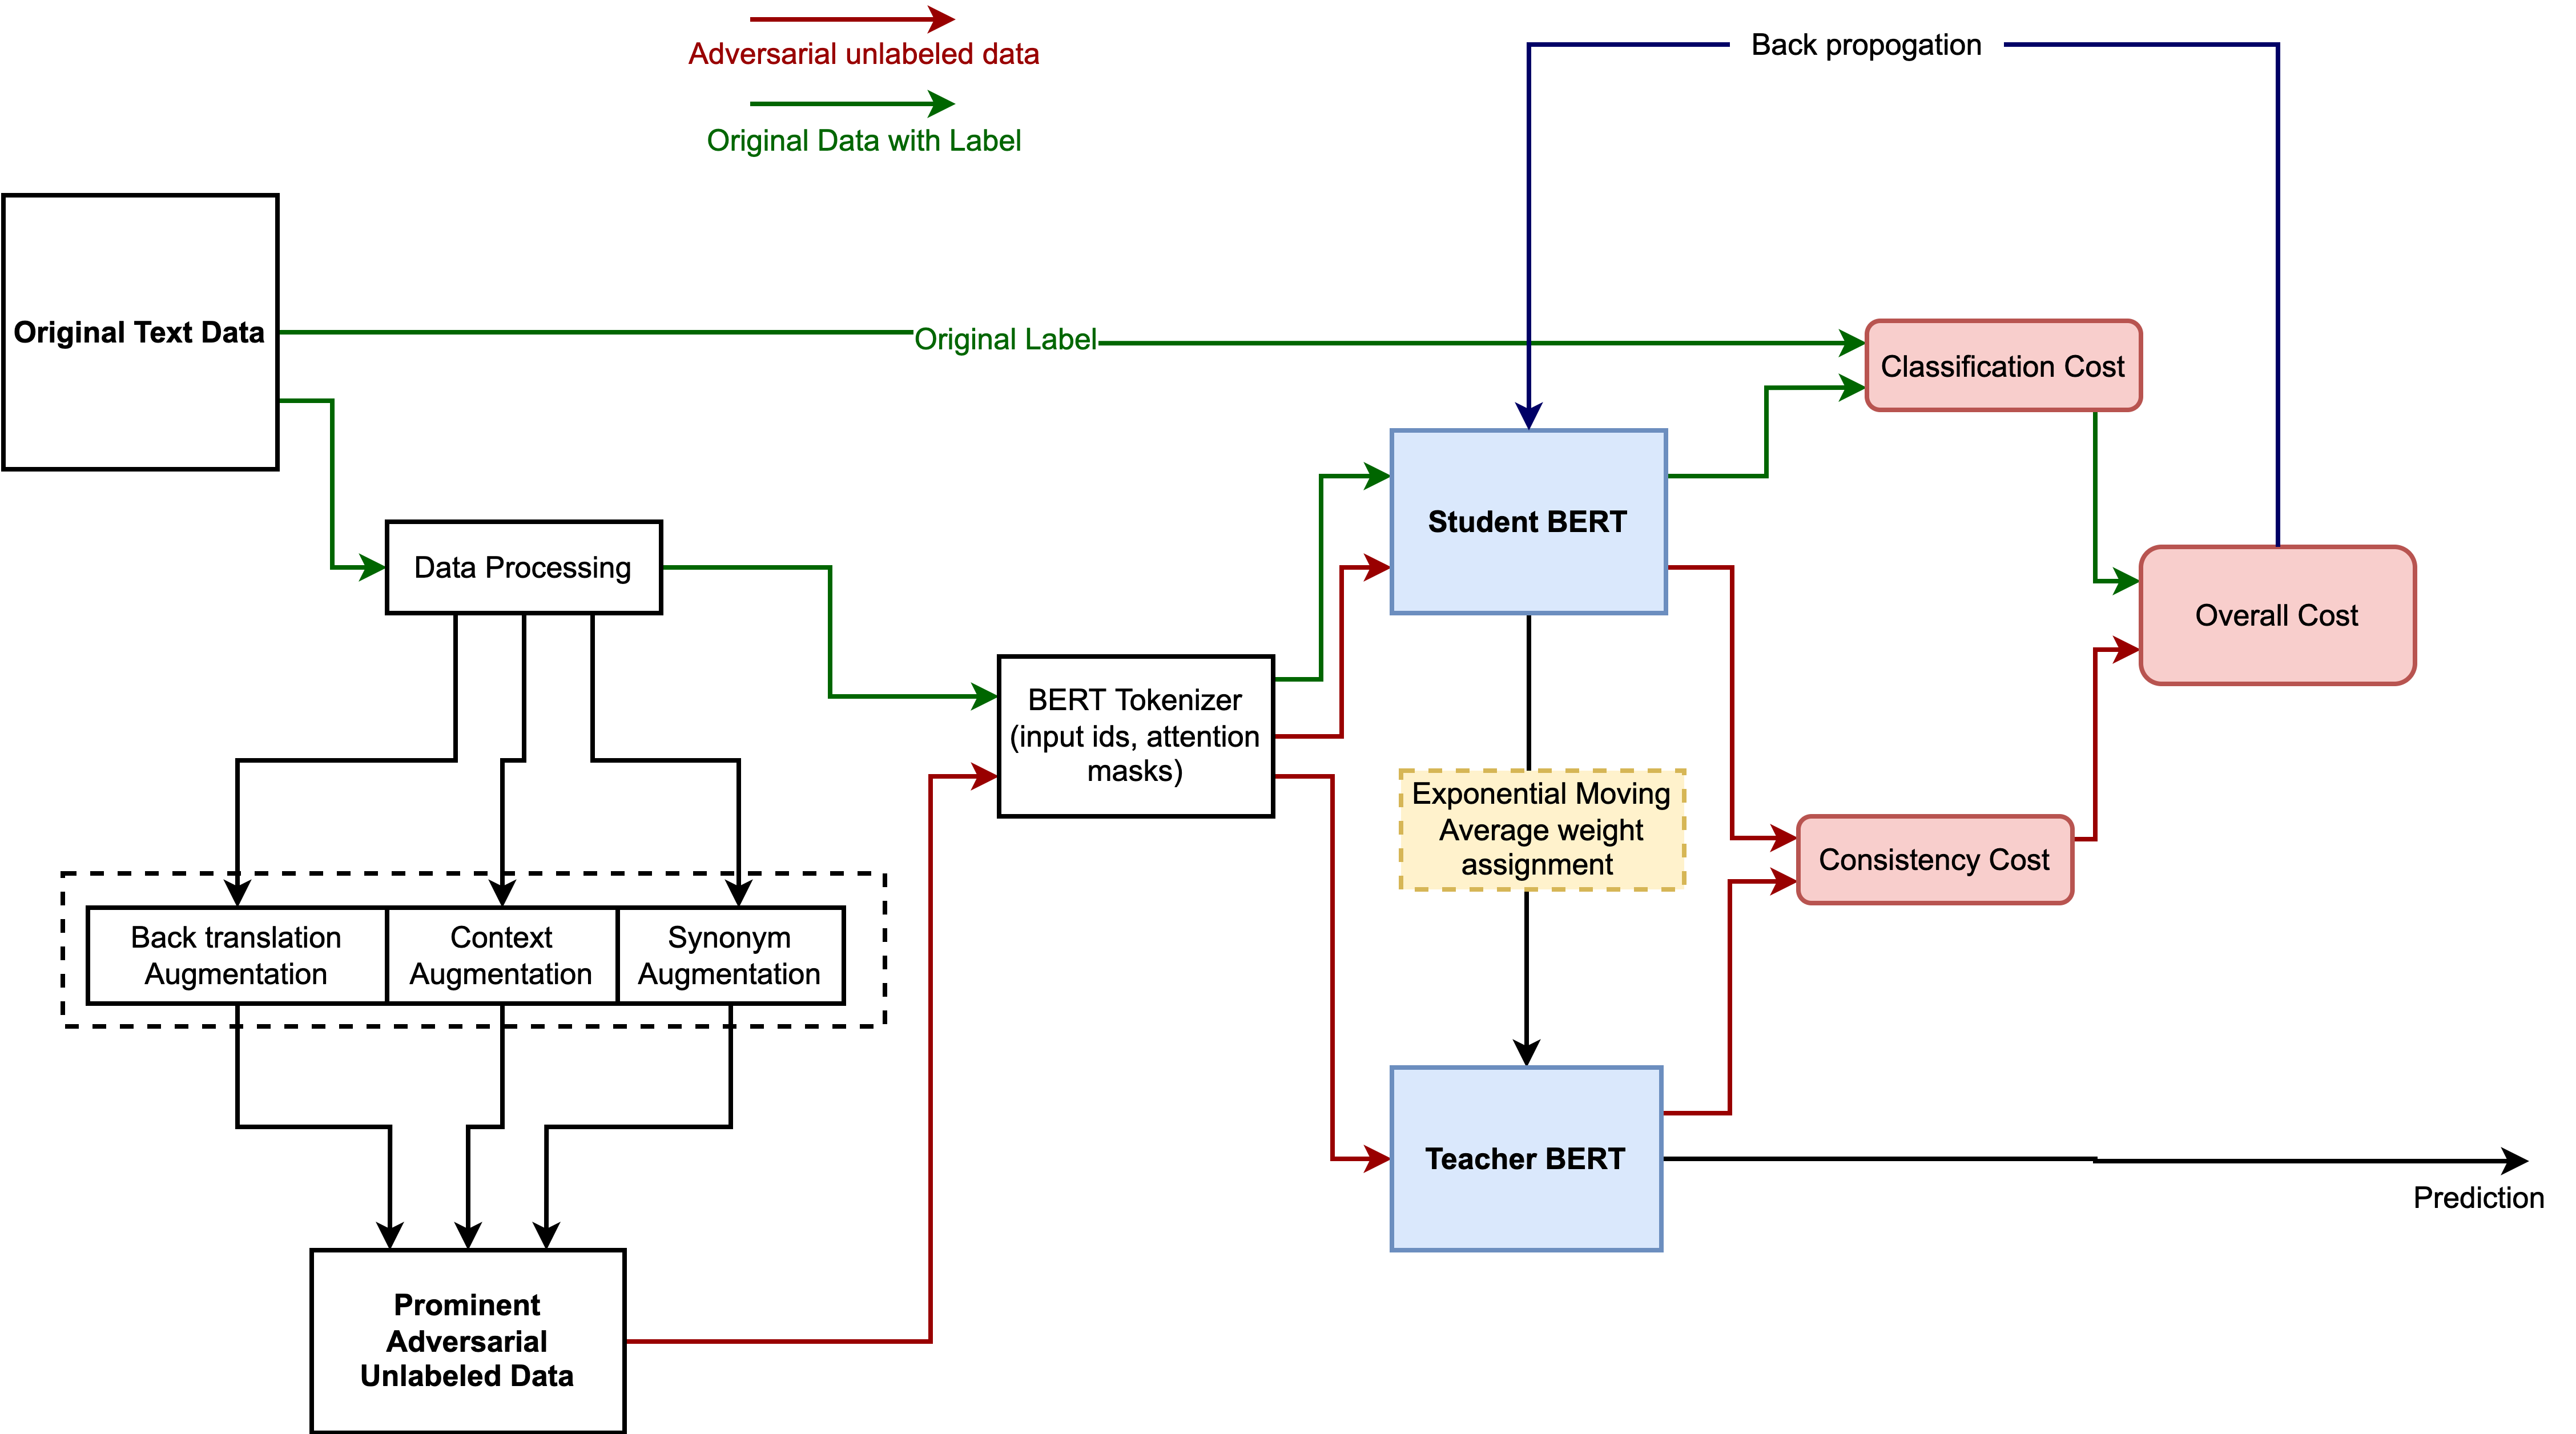
\includegraphics[width=1.1\textwidth]{img/Methodology.png}
    \caption[Training flow diagram of proposed fine-tuning approach]{Training flow diagram of proposed fine-tuning methodology }
    \label{diag:advMTBERT}
\end{figure}
The consistency cost ($J(\theta)$)  is the mean squared difference between the predicted outcomes of the student (weights $\theta$ and noise $\eta$) and the teacher model (weights $\hat\theta$ and noise $\eta'$).  The mathematical declaration is as follows. 
\begin{equation}
    \begin{aligned}
        J( \theta )=\mathbb{E}_{x_{adv}}[\|f(x_{adv},\theta)-f(x_{adv},\hat\theta)\|^2]
        \label{eq:ADVconsistencycost}
    \end{aligned}
\end{equation}
While back-propagating in the student model, the overall cost ($\textit{O}(\theta)$) is the weighted sum of classification cost ($C(\theta)$)  and consistency cost ($J(\theta)$) which can be adjusted using ratio $r$ as mentioned in the given formula 
 \begin{equation}
     \begin{aligned}
         \textit{O}(\theta)= r C(\theta)+(1-r)J(\theta)
         \label{eq:overallcost}
         \end{aligned}
   \end{equation}
   During training, exponential moving average (EMA) weights of the student model are assigned to the teacher model at every step, and the proportion of weights assigned is controlled by parameter alpha ($\alpha$). As mentioned in the equation \ref{eq:ema}, while assigning weights, the teacher model holds its previous weights in alpha ($\alpha$) proportion and ($1-\alpha$) portion of student weights. The proposed approach can be viewed as an algorithm \ref{alg:MeanTeacher}.
 \begin{equation}
     \begin{aligned}
         \hat\theta_t= \alpha\hat\theta_{t-1}+(1-\alpha)\theta_t
         \label{eq:ema}
         \end{aligned}
  \end{equation}

\begin{algorithm}[H]
    \caption{Mean Teacher Algorithm} \label{alg:MeanTeacher}
    \begin{algorithmic}
        \STATE \textbf{Data}: train set $\mathcal{(X,Y)}$,  Prominent Adversarial unlabelled set ($\mathcal{Z}$)
        \STATE \textbf{Hyper parameters}: \emph{r}, \emph{$\alpha$}, \emph{epochs}
        \STATE \textbf{Create Model}: \emph{student ($\theta$)}, \emph{teacher ($\hat\theta$)} 
        \FOR{\emph{epochs} = $1$ to $N$}
        \WHILE{$steps$}
        \STATE  \emph{student}($x$) = $y'$\
        \STATE Compute Classification cost ($C(\theta)$) = Binary Cross Entropy($y$,$y')$
        \STATE  \emph{student}($z$) = $y_s$
        \STATE  \emph{teacher}($z$) = $y_t$
        \STATE Compute Consistency cost $J(\theta)$=Mean Squared Error($y_s$,$y_{t}$)
        \STATE Compute Overall cost  $\textit{O}(\theta)= r C(\theta)+(1-r)J(\theta)$
        \STATE Compute \emph{gradients}, \textit{O}($\theta$) w.r.t  $\theta$ 
        \STATE Apply \emph{gradients} to $\theta$
        \STATE Update Exponential Moving average of $\theta$ to $\hat\theta$ i.e. $\hat\theta_t= \alpha\hat\theta_{t-1}+(1-\alpha)\theta_t$\
        \ENDWHILE
        \ENDFOR
    \end{algorithmic}
\end{algorithm}

\section{Text Attack Recipes and Tool}
\label{section:attackrecipes}
To evaluate the proposed approach, four black box attack recipes that satisfy lexical, grammatical, and semantic constraints have been selected. To conduct the experiment, TextAttack python package \cite{morris_textattack_2020} is used to utilize these attack recipes. The table \ref{table:attackRecipeExample} shows  examples of perturbation created in this experiment. Attack recipes  working principles and characteristics are discussed in this section. 

\begin{table}[h!]
    \centering
    \hspace*{-1.2em}
    \resizebox{1.0\textwidth}{!}{
            \begin{tabular}{|p{3 cm}|p{9cm}|p{9cm}|}
                \hline
                Attack Recipe & Original Text & Perturbed Text \\
                \hline
                TextFooler & absolutely \textcolor{red}{fantastic} whatever i say wouldn t do this underrated movie the justice it deserves watch it now fantastic	 & absolutely  \textcolor{red}{sumptuous}  whatever i say wouldn t do this underrated movie the justice it deserves watch it now fantastic	 \\
                \hline
                TextBugger & absolutely \textcolor{red}{fantastic} whatever i say wouldn t do this underrated movie the justice it deserves watch it now fantastic	 & absolutely \textcolor{red}{fa?tastic} whatever i say wouldn t do this underrated movie the justice it deserves watch it now fantastic	 \\
                \hline
                PWWS & absolutely \textcolor{red}{fantastic} whatever i say wouldn t do this underrated movie the justice it deserves watch it now fantastic	 & absolutely \textcolor{red}{rattling} whatever i say wouldn t do this underrated movie the justice it deserves watch it now fantastic	 \\
                \hline
                BAE & absolutely \textcolor{red}{fantastic} \textcolor{red}{whatever} i say wouldn t do this underrated \textcolor{red}{movie} the justice it deserves \textcolor{red}{watch}  it now fantastic	 & absolutely \textcolor{red}{shit}   \textcolor{red}{something}  i say wouldn t do this underrated \textcolor{red}{film}   the justice it deserves  \textcolor{red}{of}  it now fantastic	 \\
                \hline
            \end{tabular}
              }
        \caption[ Perturbation examples of attack recipes.]{ Perturbation examples of attack recipes in this experiment.}
        \label{table:attackRecipeExample}
\end{table}

\subsection{TextFooler}
\label{subsection:textfooler}
Jin \textit{et al.} \cite{jin_is_2020-1} proposed TextFooler, a simple and effective adversarial attack generation strategy in black box settings which has characteristic of preserving the semantics, and grammar. The utility-preserving adversarial examples is illustrated in figure \ref{diag:TextFoolerExp}. For better understanding, the process is briefly explained in steps:
\begin{enumerate}
    \item  \textbf{Word Importance Ranking}: Given a sentence of words, they create a ranking of each word by measuring the change before and after deleting the words, called the importance score. NLTK and spaCy libraries are used to remove words and preserve the grammar of the sentences. To improve the similarity of vectors, antonymy, and synonymy are injected into vector space representations.\\
    The replacement policy completely depends on three factors: 1) Similar semantic similarity, 2) Fit in the surrounding context, 3) Attack on the model. Universal Sentence Encoder \cite{cer_universal_2018} is used in this study for encoding the sentence into a high-dimensional vector and calculating the cosine similarity between the sentences. Next, replacing candidates with values above the preset threshold value and creating a pool of candidates.
    \item \textbf{Replacement}: A candidate from pool of candidates who can change the prediction of a target model is selected which has the highest cosine similarity between the original and adversarial sentences. If not, a lower confidence score for the label is chosen.
\end{enumerate}
Using IMDB movie review datasets, TextFooler has assessed the performance of the BERT model under adversarial attacks. In their experiment, the accuracy dropped significantly from 90.9\% to 13.6\% with 6.1 average perturbed words, 1134 number of queries,, and the average length of IMDB dataset was 215. Furthermore, TextFooler is computationally inexpensive and complexity increases linearly with text length. 
\begin{figure}[H]
    \centering
    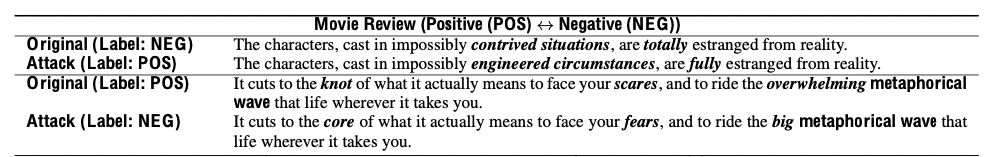
\includegraphics[width=1.0\textwidth]{img/textfooler_example.png}
    \caption[Example of TextFooler]{TextFooler example  \cite{jia_certified_2019} }
    \label{diag:TextFoolerExp}
\end{figure}

\subsection{TextBugger}
\label{subsection:textbugger}
The TextBugger system proposed by Li \textit{et al.} \cite{li_textbugger_2019} uses misspelled words or characters that are visually and semantically similar to the original text. When tokens are misspelled, they become 'Unknown,' which is mapped to unknown token ids, causing machine learning models to behave incorrectly. On the other hand, studies show that similar misspellings can still be perceived by the reader \cite{rawlinson_significance_2007,alzantot_generating_2018}. Both character-level and word-level perturbation are targeted in this attack. Although Li \textit{et al.} \cite{li_textbugger_2019}  proposed both white box and black box attack generation strategies, our report focuses on black-box attacks. Here are three steps to black-box attack generation:
\begin{enumerate}
    \item \textbf{Finding Important Sentences}: The importance score of individual sentence in an article is determined by the confidence score of that sentence by the target model.
    \item \textbf{Finding Important Words}: The importance score of a word is the difference between the confidence of the target model with a word and without a word.
    \item \textbf{Bugs Generation}: In TextBugger, five bug generation strategies are utilized 1) \textbf{Insert}: Inserting space into words, 2) \textbf{Delete}: Deleting random character,
    3) \textbf{Swap}: Swapping random adjacent character, 4) \textbf{Substitute-C}: Substitute character with visually similar characters, and 5)\textbf{ Substitute-W}: Replacing a word with the top-k nearest neighbour in context-aware word vector space, as shown in figure \ref{diag:textbug}
\end{enumerate}

\begin{figure}[H]
    \centering
    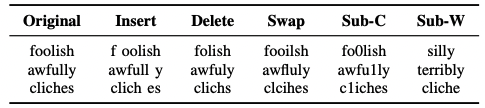
\includegraphics[width=.65\textwidth]{img/textbugger_5strat.png}
    \caption[Example of 5 bug generation strategies of TextBugger]{TextBugger 5 bug generation strategies \cite{li_textbugger_2019} }
    \label{diag:textbug}
\end{figure}
In their study, evaluation is conducted using the IMDB movie review dataset and sequential models. As per their result, Logistics Regression, CNN, and LSTM  showed 95.2\%, 90.5\%, and 86.7\% success rate with perturbed words of 4.9\%, 4.2\%, and 6.9\%, respectively. But, their study did not assess the effectiveness of the BERT model. TextBugger generates adversarial attacks quickly than TextFooler because of its sub-linear relationship to text length.

\subsection{Generating Natural Language Adversarial Examples through Probability Weighted Word Saliency (PWWS)}
\label{subsection:generatingadversarialexample}
Ren \textit{et al.} \cite{ren_generating_2019} proposed a method for synonym and named entity (NE) replacement based on the words' saliency and classification probability, as well as a greedy algorithm called Probability Weighted Word Saliency (PWWS). When replacing a word with suitable synonym, there must be a significant change in classification probability as well as shows minimum saliency of the word. The approach can be summarized as follows:

\begin{enumerate}
    \item \textbf{Word Selection Strategy}:  
   The salience of a word is defined as its degree of change in classification probability if the word is set to unknown \cite{li_understanding_2017}. Calculating word saliency vectors for each word in a text, and then prioritizing the words based on the degree of change in classification probability and word saliency.  
    \item \textbf{Replacement Strategy}: They have used WordNet for the search of word synonyms to find the replacement. Also, if the word is a Named Entity (NE), then replacing it with another NE of the same type appeared in the opposite class.
\end{enumerate}
Lastly, greedily replacing the words to attach the model. According to the result, the accuracy dropped from 84.86\% to 2.00\% with perturbation 3.38\% for the IMDB dataset and Bi-LSTM model, example is shown in figure \ref{diag:pwwsexp}. However, the computational and time complexity of the proposed approach is higher than other methods.
\begin{figure}[H]
    \centering
    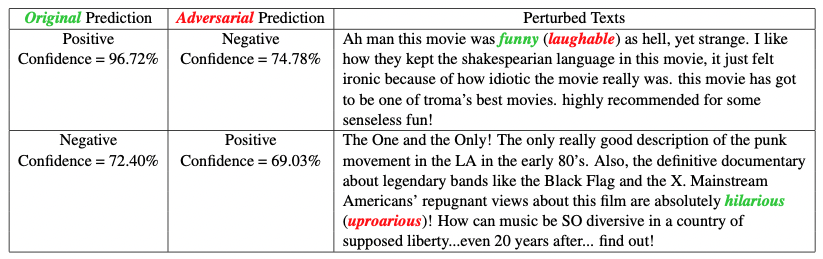
\includegraphics[width=0.95\textwidth]{img/PWWSexample.png}
    \caption[Example of PWWS attack recipe]{Example attack of PWWS\cite{ren_generating_2019} }
    \label{diag:pwwsexp}
\end{figure}

\subsection{BAE: BERT-Based Adversarial Examples}
\label{subsection:bae}
The BERT masked language model (MLM) was employed by Garg \textit{et al.} \cite{garg_bae_2020}  to generate adversarial examples. Based on their approach, they first calculate the importance of words by computing the decrease in probability of predicting the correct label after deleting that particular word, similar to Textfooler \cite{jia_certified_2019}  and PWWS \cite{ren_generating_2019}. Using the BERT MLM model, replace a specific word with a MASK token and let the model predict context-specific masked words. \\
Using the Universal Sentence Encoder \cite{cer_universal_2018},  removing words that do not fall into a similar part-of-speech (POS) as the original word, and then filtering the top K tokens using the similarity score (Threshold 0.8). Later, substituting top K (50) tokens for the original word and iterating through the most similar token in decreasing order until the attack is successful and then trying all combinations. Figure \ref{diag:baeexp} shows a schematic working diagram.
\begin{figure}[H]
    \centering
    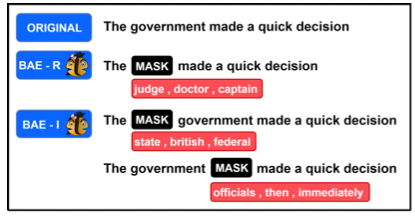
\includegraphics[width=.59\textwidth]{img/BAEexample.png}
    \caption[Schematic working and example of BAE attack recipe]{Schematic working and example of BAE \cite{garg_bae_2020} }
    \label{diag:baeexp}
\end{figure}
 
\chapter{Experiment Setup}
\label{chapter:experiment}

\section{Dataset}
\label{label:dataset}
To assess the performance of baseline and proposed model, two binary classification datasets were selected i.e. 1) Covid-19  fake tweets dataset \cite{patwa_fighting_2021} provided by Codalab, and 2) IMDB movies review \cite{maas_learning_2011-1}. \\
The IMDB dataset is a sentiment classification dataset contains user movie reviews labelled as positive and negative. In addition, this dataset is majorly used for evaluation in classification and adversarial attack studies. Due to computational limitations, we have filtered and sampled only datasets whose length is between 6 and 150 as the augmentation process takes quite a while. This provided 8050 samples to train and test our model. The train and test sizes are shown in table \ref{table:train/testtable}. Additionally, 6050 dataset is sampled to create augmented unlabelled dataset and the filtered datasets have an average text length of 127. The label distribution in training datasets is completely balanced.\\
Covid-19 fake tweets dataset is a recent dataset specifically for classifying fake tweets as fake or real. Covid-19 fake tweets dataset sized 8000 and this dataset is fully utilized in the experiment. Contrary to the IMDB dataset, the Covid-19  fake tweets dataset has an average length of 25, as shown in table \ref{table:Length stat }. Furthermore, as Covid-19  fake tweets dataset has mostly hashtags and comparatively lower vocabulary size. Therefore, the intention of observing the models behaviour under a recent dataset that has comparatively lesser text length and vocabulary size led to selecting this dataset.

\begin{table}[!h]
\centering
\begin{tabular}{ |c|c|c|c|c|c| }
\hline
Dataset & Train & Test  & Aug. unlabelled \\
\hline
codalab (Positive/Negative) & 3199/2891 & 1071/969 & 6090 \\
\hline
IMDB (Fake/Real) & 3025/3025 & 1000/1000 & 6050  \\
\hline
\end{tabular}
\caption[Train/Test/Unlabelled details of dataset]{Train/ Test split details of dataset }
\label{table:train/testtable}
\end{table}

\section{Data Pre-processing and Exploration}
\label{section:datapreproc}
Due to the fact that language models learn context from sentences, they are least affected by stop words, and removing those words may affect the performance. Language models offer the benefit of negligible data cleaning, which is one of their benefits. The pre-processing steps involved in this experiment as follows:
\begin{enumerate}
\item  HTML tags removal.
\item Digit removal.
\item Lower casing.
\item  Punctuation removal.
\end{enumerate}
This particular task was accomplished by using the texthero python library, which offers functions related to data pre-processing and exploration.
\subsection{Data Exploration}
\label{subsection:dataexploration}
In the experiment, models were trained with almost equal distributions of labels and the same training data is being used to generate unlabelled augmented data is shown in \ref{table:train/testtable}. During experiments, various exploration techniques were utilized such as word cloud, word length distribution, and word distribution with/without respect to classes are studied during experiment. However, the most relative information about the dataset i.e. about length is provided in the table \ref{table:Length stat } and figure \ref{fig:lendist}.
\begin{table}[!h]
\centering
\begin{tabular}{ |c|c| }
\hline
Dataset &  Avg. Length  \\
\hline
codalab & 25  \\
IMDB & 127  \\
\hline
\end{tabular}
\caption[Length details of datasets]{Length details of both the datasets.}
\label{table:Length stat }
\end{table}
\begin{figure}[H]
     \hspace*{-.7em}
    \begin{minipage}[b]{0.5\linewidth}
        \centering
        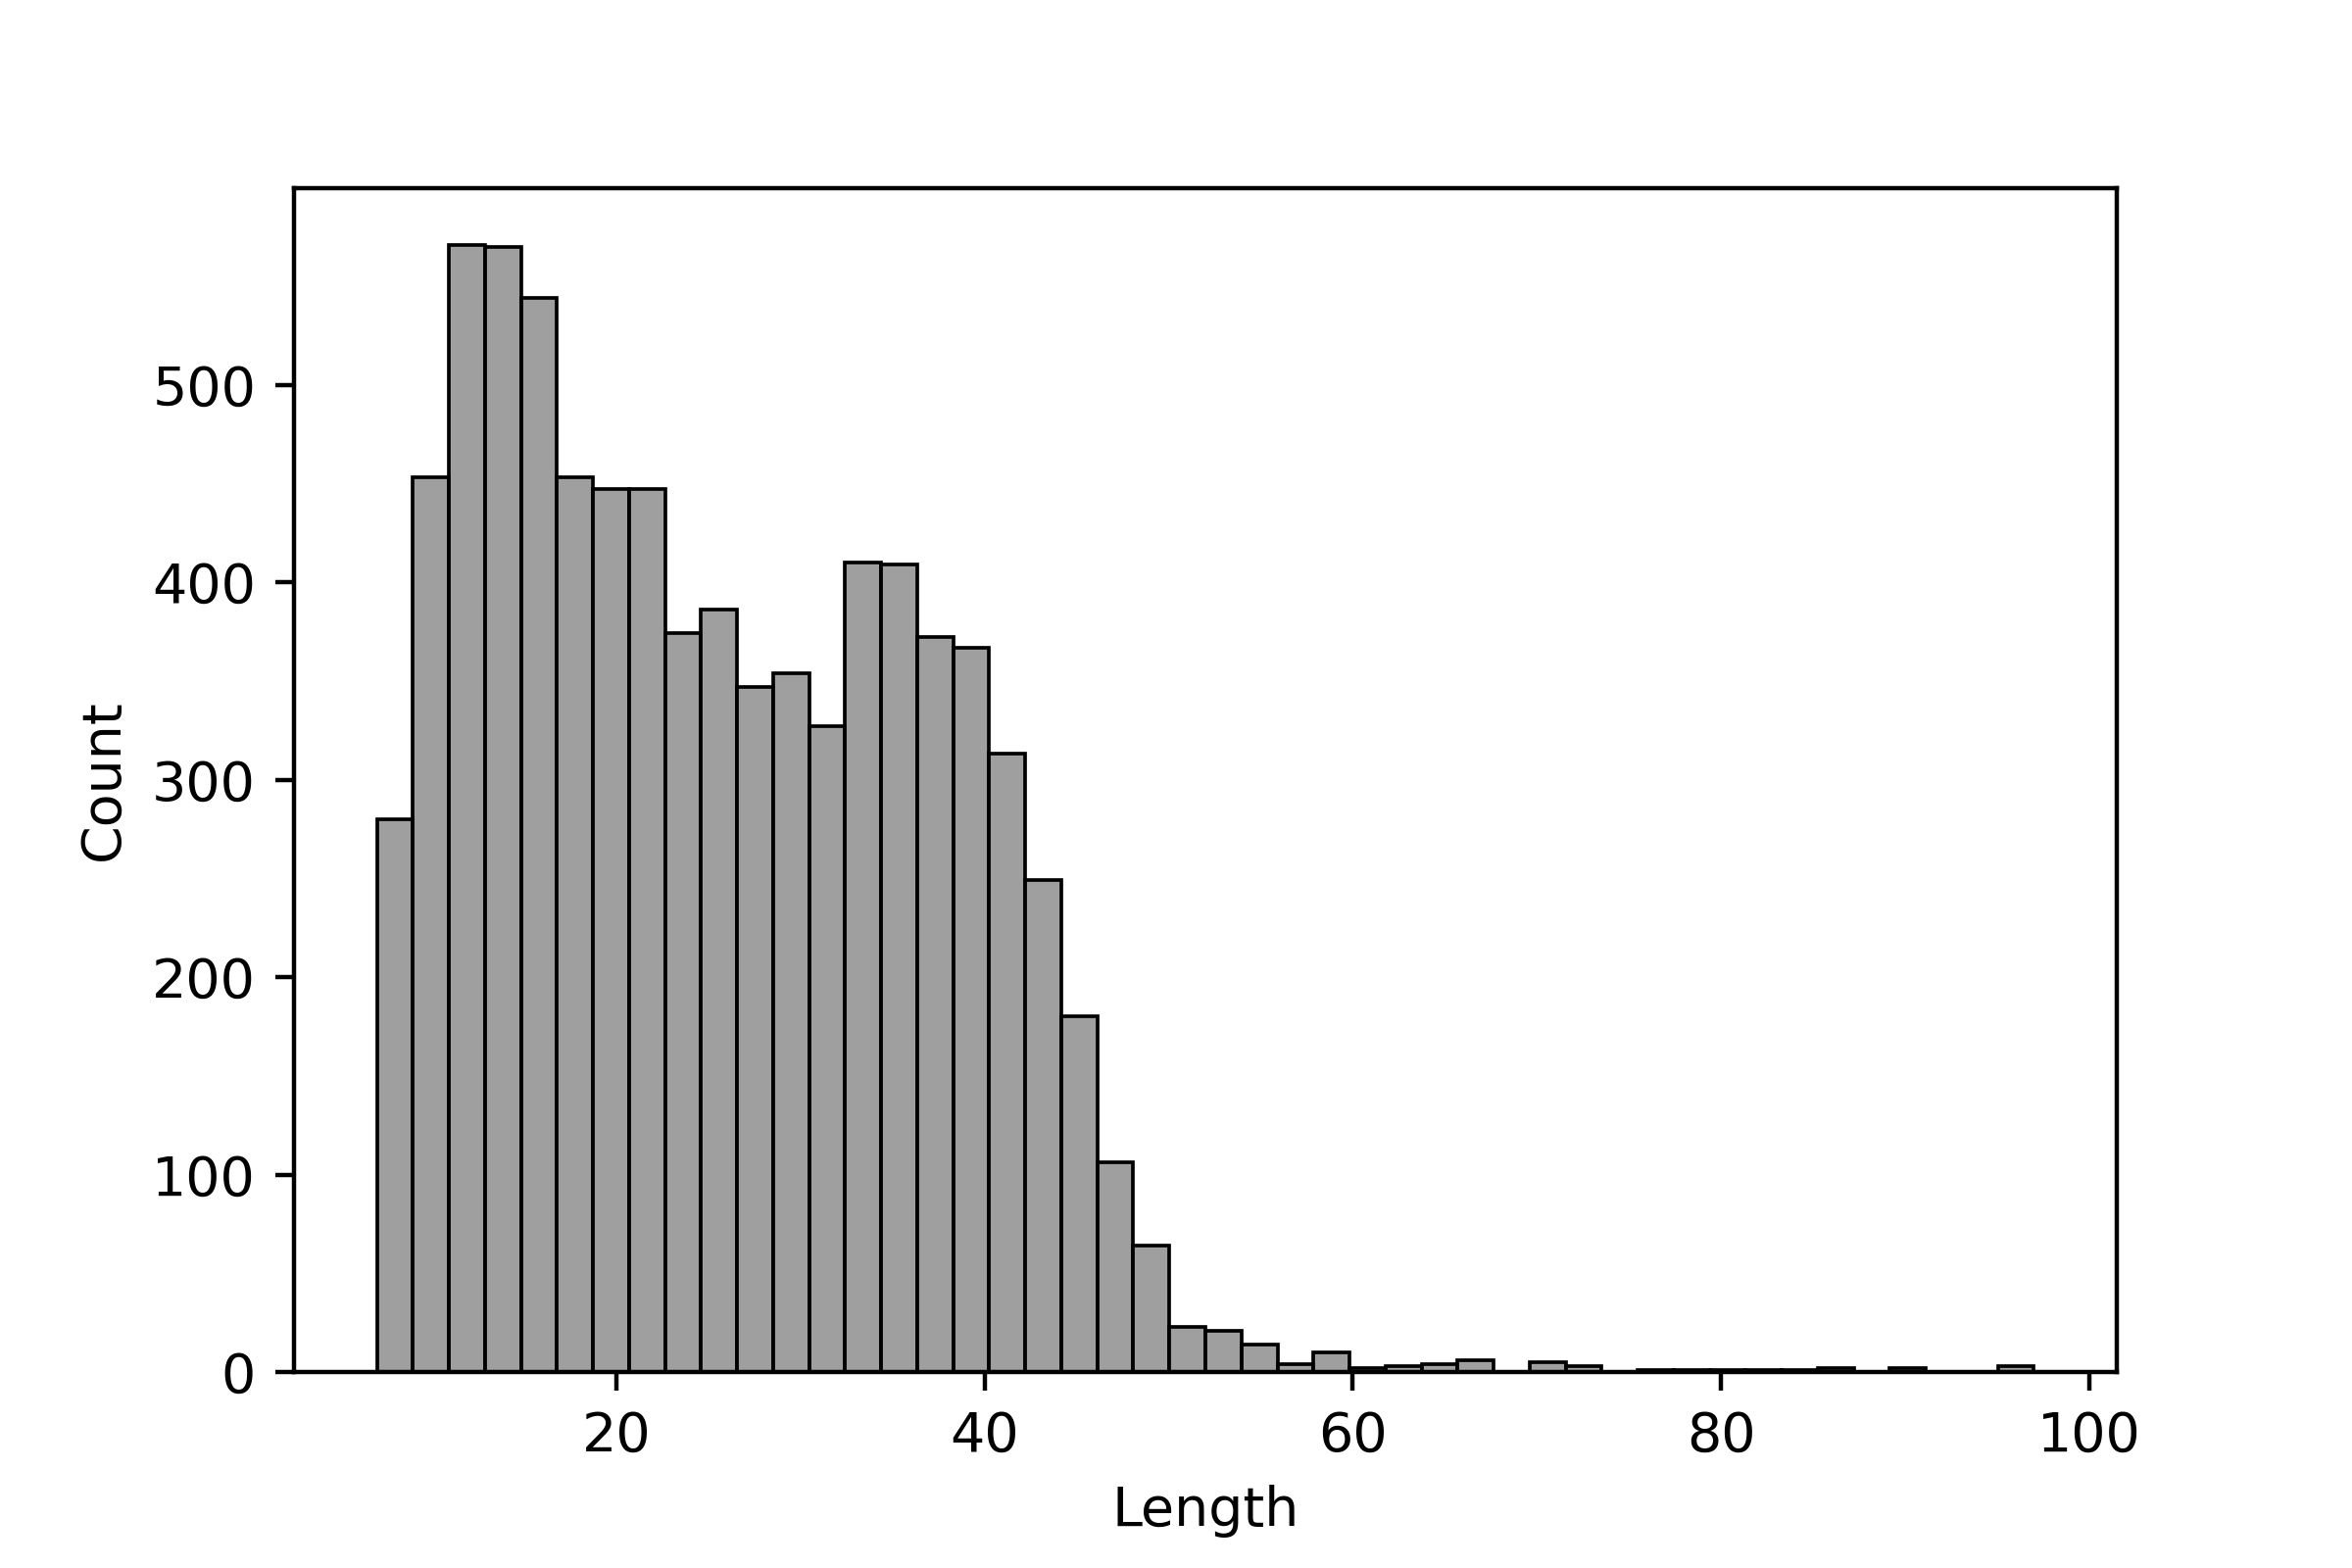
\includegraphics[width=\textwidth]{img/fakenewsLengthdist.png}
        \caption{Length distribution of Covid-19 fake tweets dataset.}
        \label{fig:fklendist}
    \end{minipage}
    \hspace{0.1cm}
    \begin{minipage}[b]{0.5\linewidth}
        \centering
        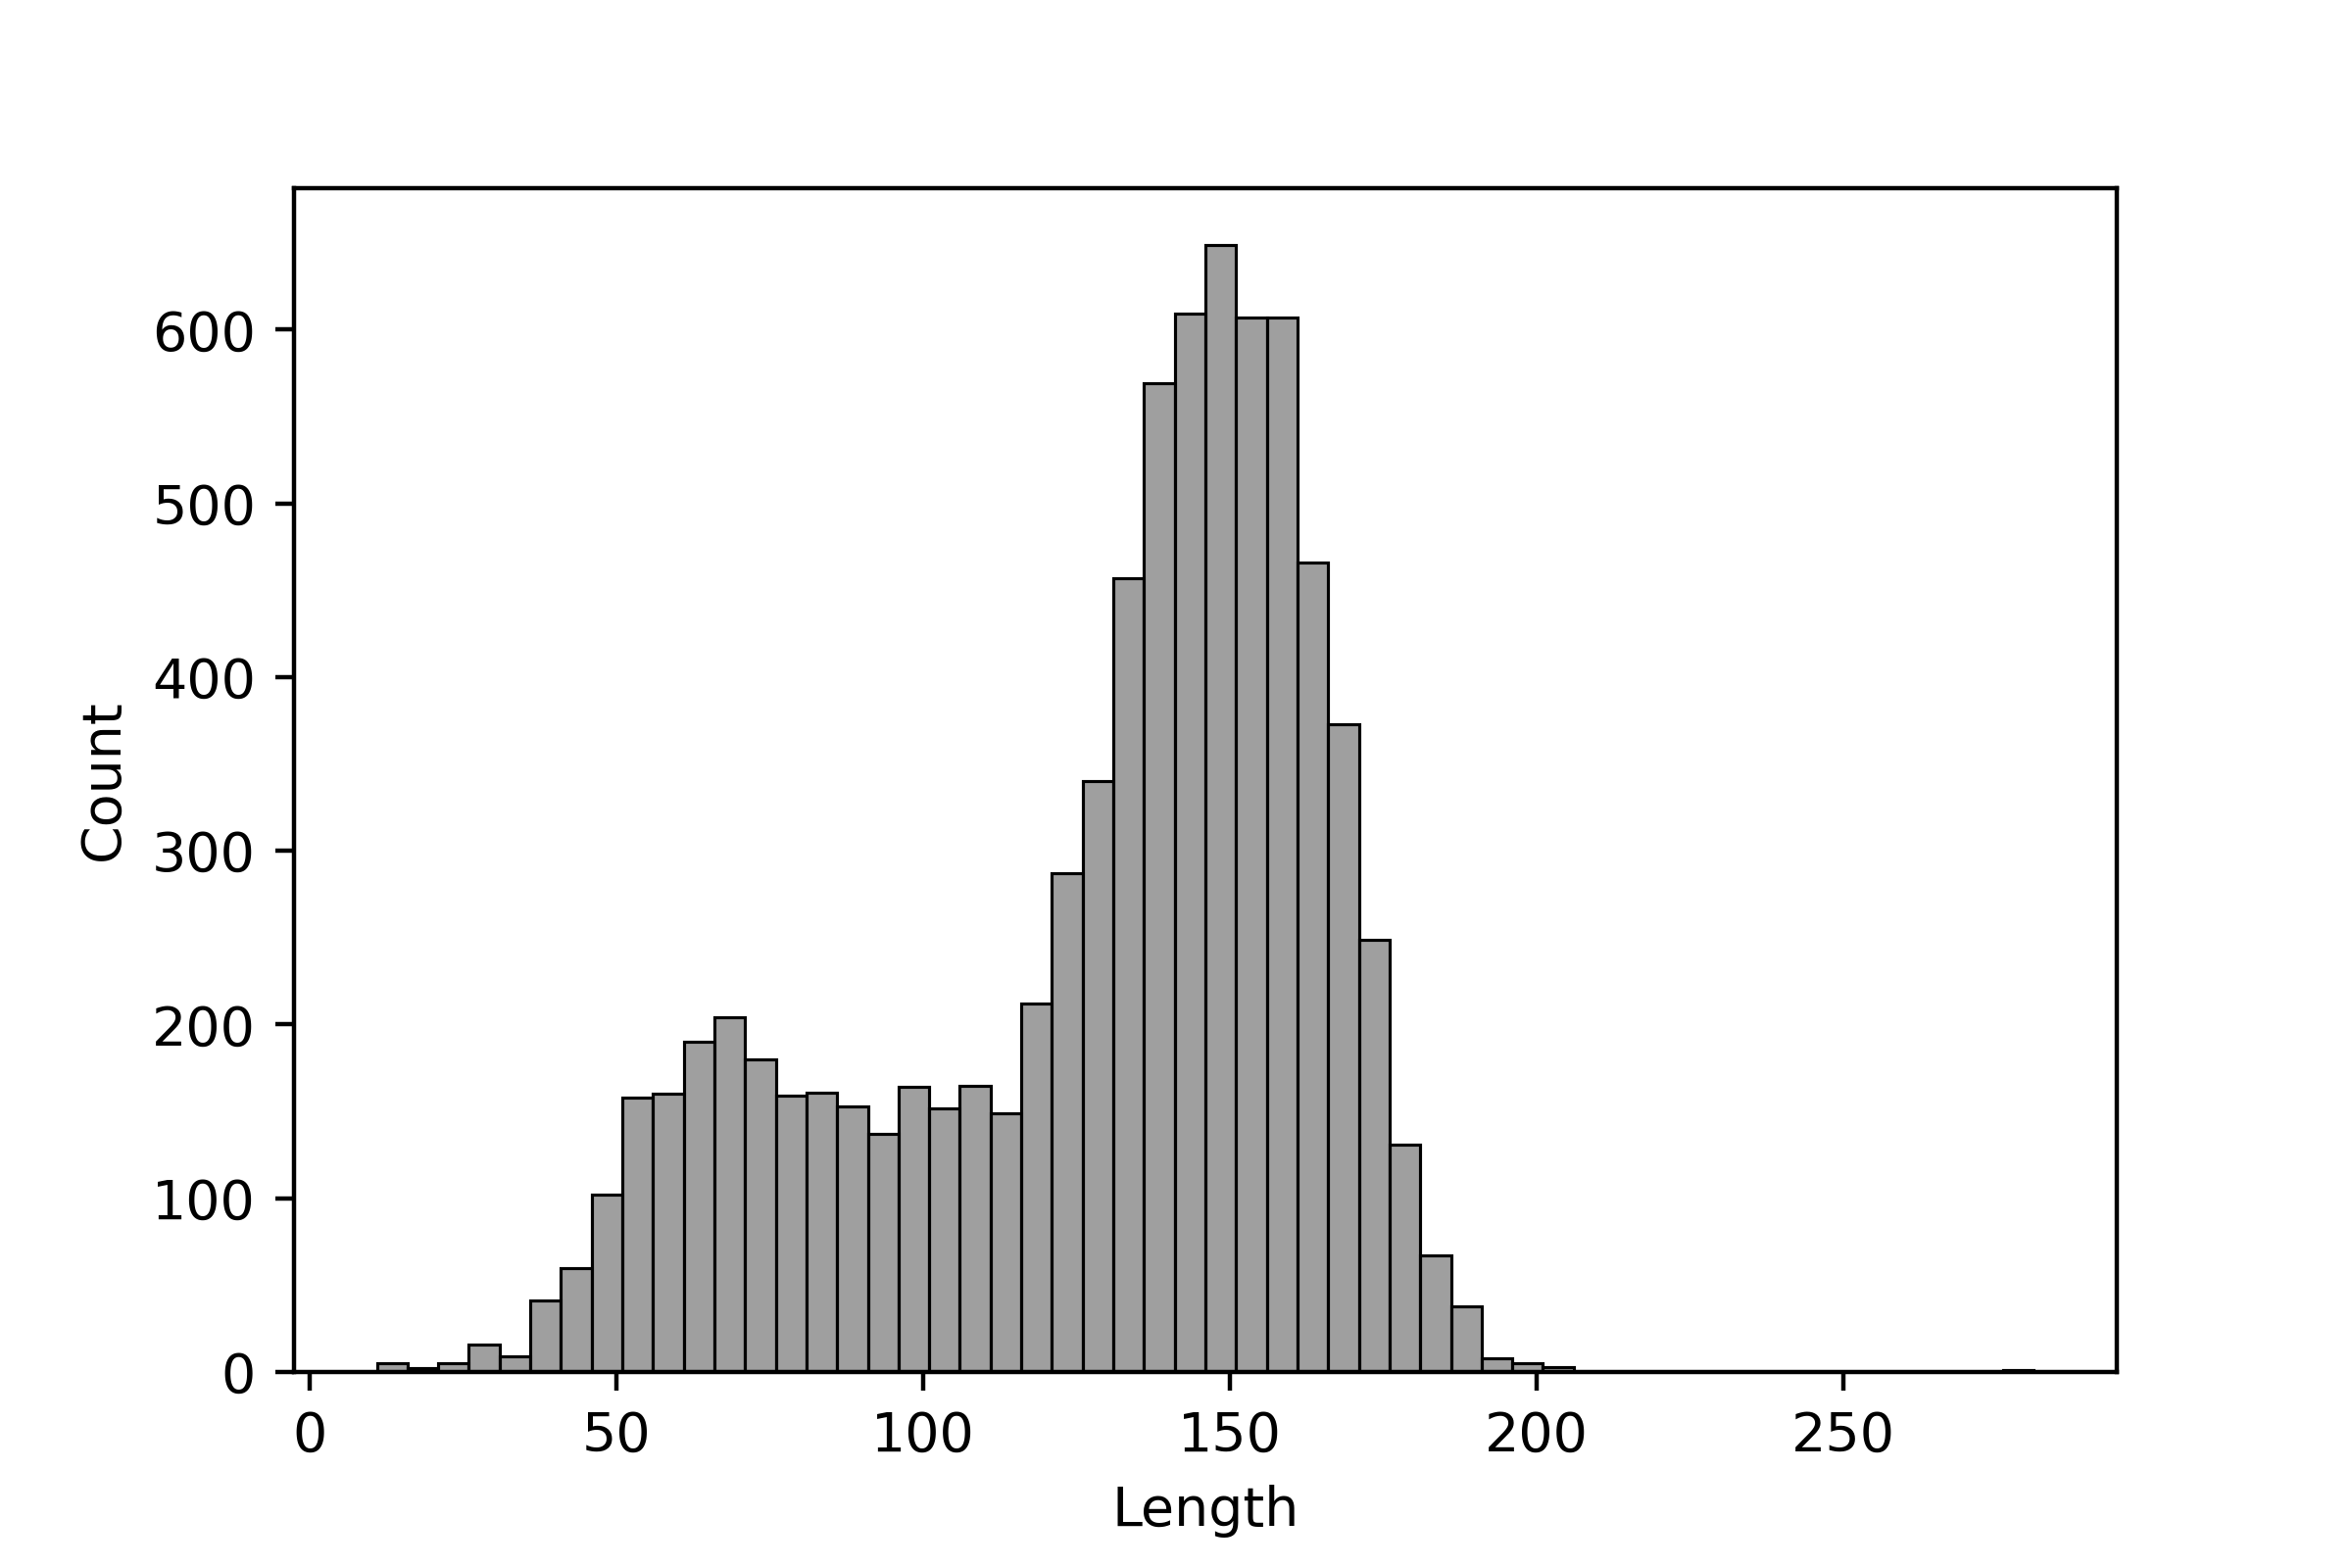
\includegraphics[width=\textwidth]{img/ImdbLengthdist.png}
        \caption{Length distribution of IMDB dataset.}{}
        \label{fig:imdblendist}
    \end{minipage}
    \caption[Length distribution of Covid-19 fake tweets and IMDB dataset]{\small Length Distribution of Covid-19 fake tweets and IMDB dataset.}
    \label{fig:lendist}
\end{figure}
The Covid-19 Fake tweets dataset  length is comparatively shorter than the IMDB dataset. The purpose of using two distinct length datasets is to better understand the behaviour of models and attack recipes in relation to the length.
%\begin{figure}[H]
%    \centering
%%    \hspace*{1.0em}
%    \begin{subfigure}
%        \centering
%        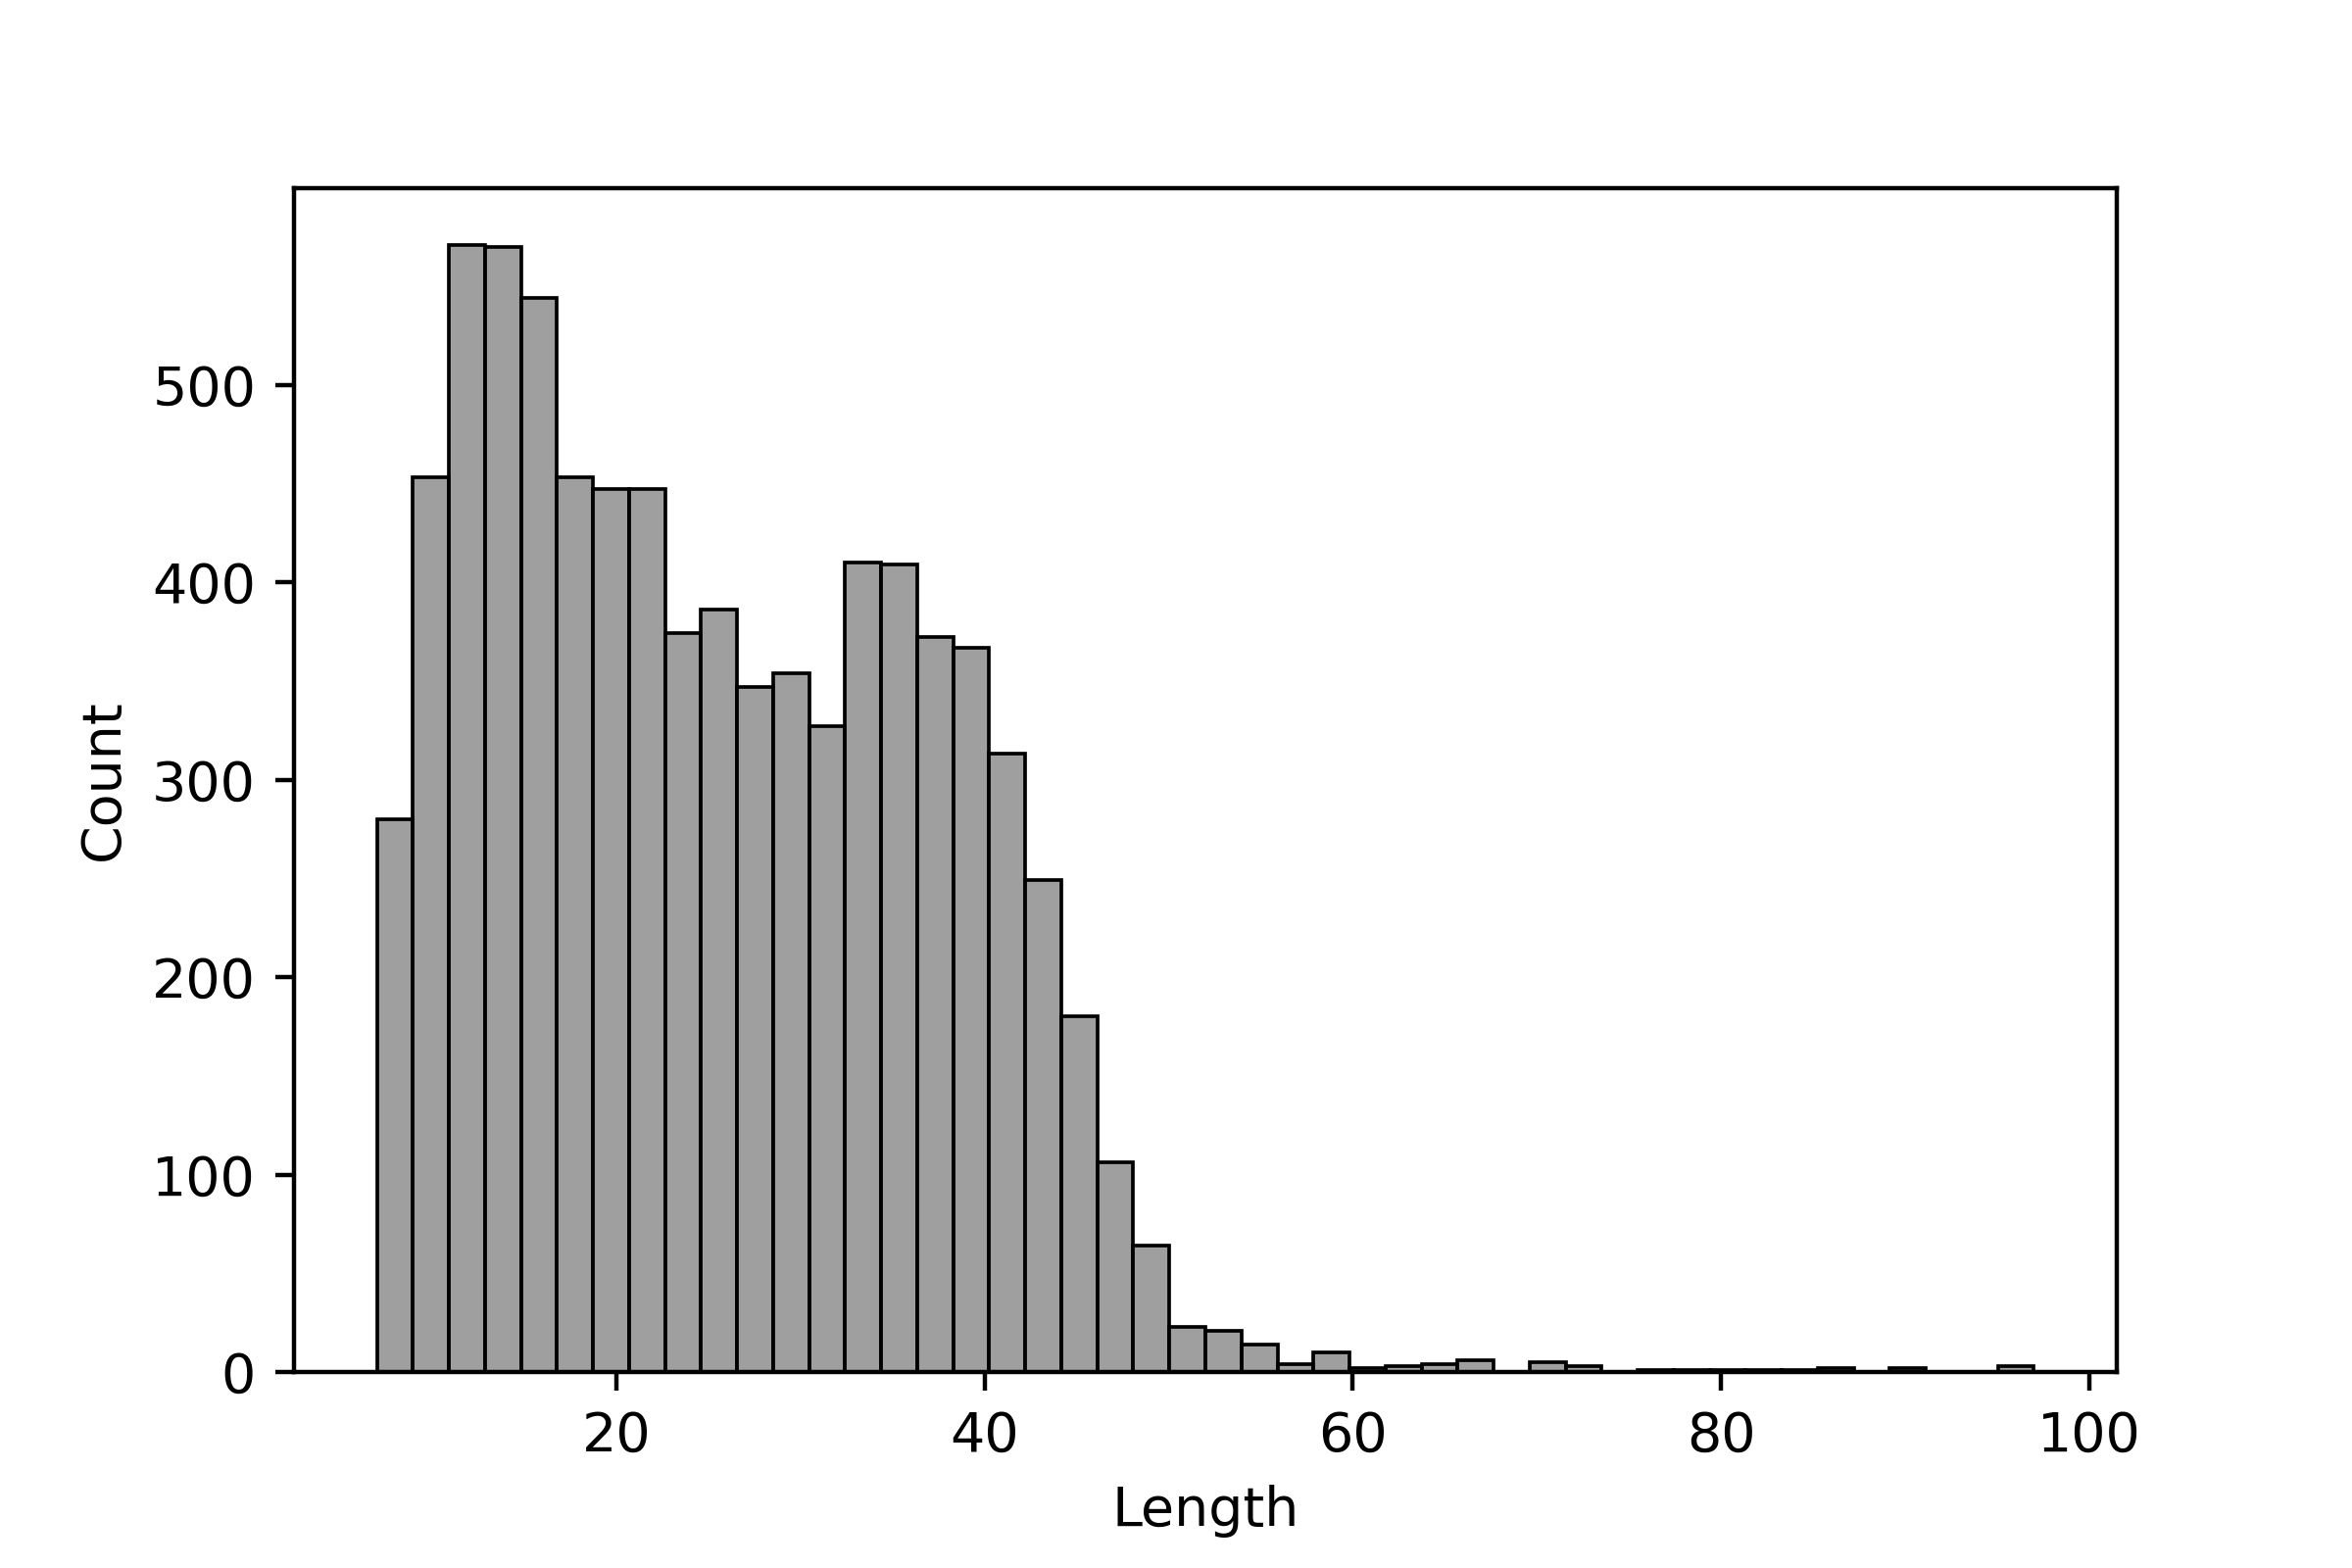
\includegraphics[width=.5\linewidth]{img/fakenewsLengthdist.png}
%        \caption{Covid-19 fake tweets dataset.}{}
%           \label{fig:}
%    \end{subfigure}
%%    \hspace*{1.8em}
%    \begin{subfigure}
%        \centering
%        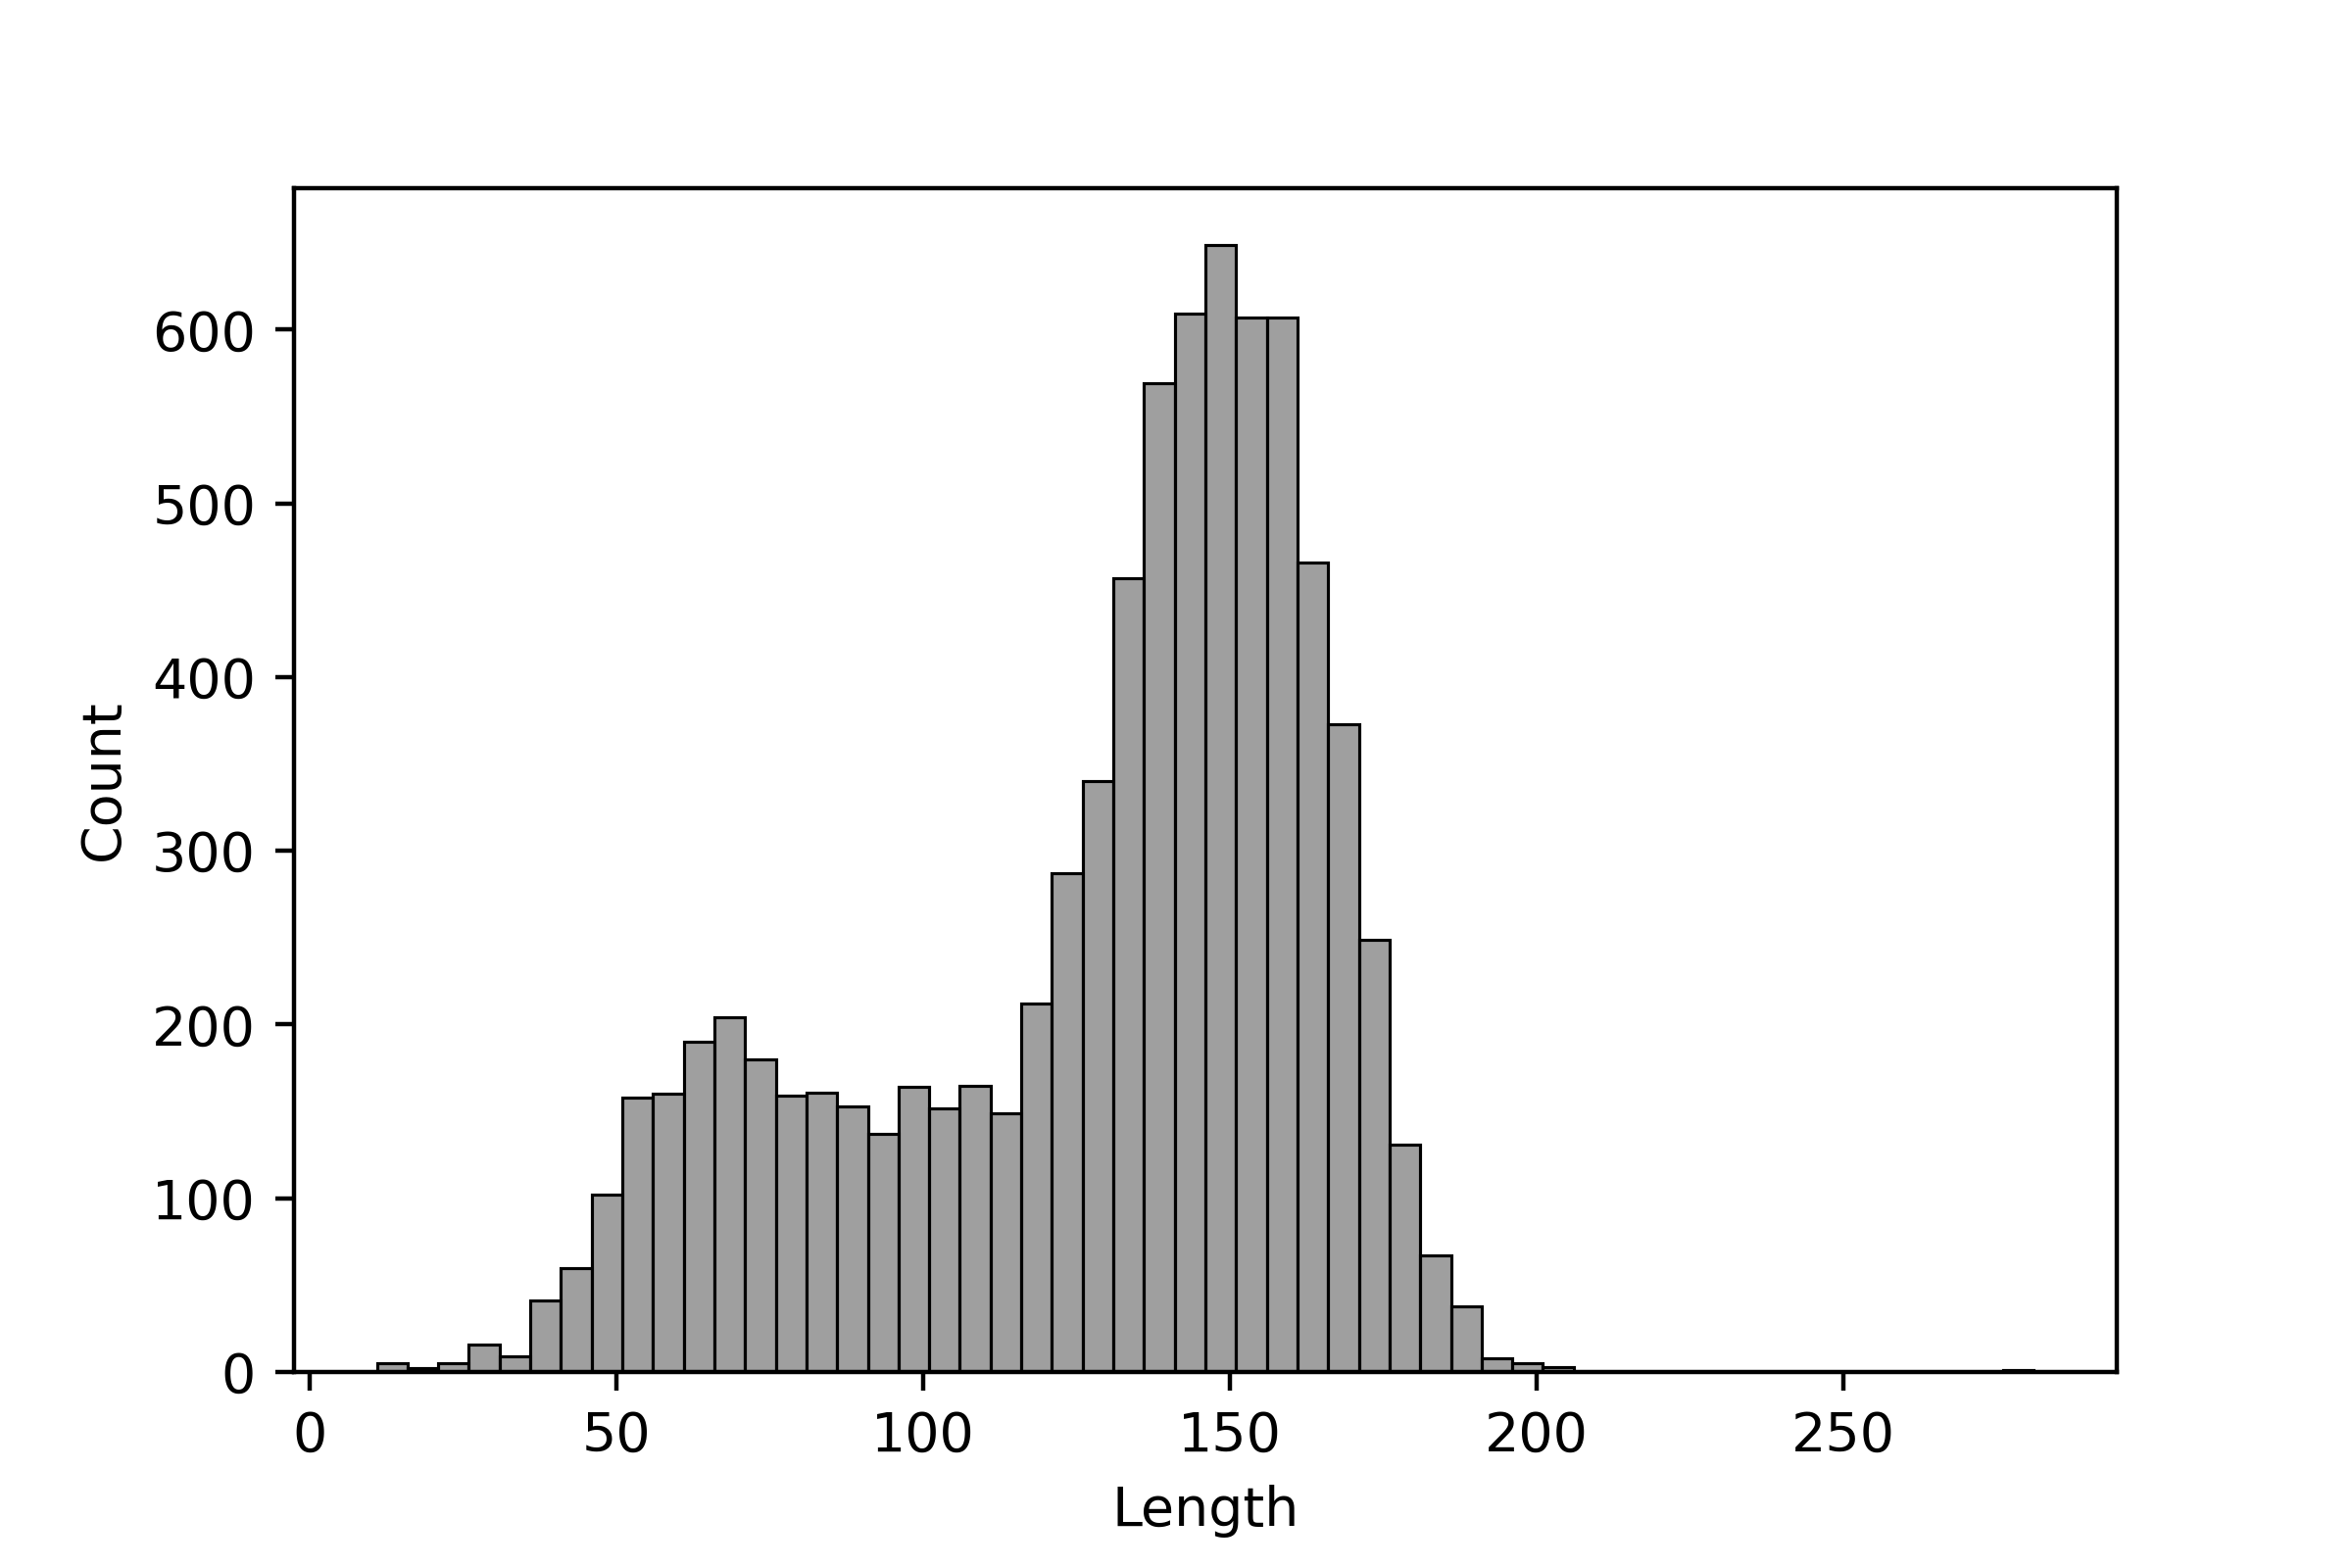
\includegraphics[width=.5\linewidth]{img/ImdbLengthdist.png}
%        \caption{IMDB Dataset.}{}
%          \label{fig:sub2}
%    \end{subfigure}
%\caption{Length Distribution of Fake news and IMDB Dataset.}{}
%\end{figure}

\section{Data Augmentation}
\label{section:dataaugmentation}

For creating the unlabelled augmented dataset, we have utilized three strategies i.e. 1) Synonym-based, 2) Context-based, and 3) Back translation.
In this experiment, while augmenting it was observed that the information is changed or completely opposite to the class of the original dataset. Therefore, labels were dropped, hence, called unlabelled data. 
%\subsubsection{Synonym Based}
For synonym changes, various python packages like text attack, nlpaug, and various basic python packages were used during experiments.\\
In addition, time and computation constraints have led us to choose the nlpaug\footnote{https://github.com/makcedward/nlpaug} data augmentation package  to achieve all three augmentation strategies. The labels of training dataset were dropped while creating augmented dataset and then, randomly splitting it into three parts. The first part is for synonym augmentation, the second part is for context-based augmentation, and the last part is for back-translation. \\
In another scenario, unlabelled data created using different attack recipes can provide better results under attacks. The intention of this experiment was to create a model without understanding of attack recipes, hence, not utilizing for augmentation. Furthermore, utilizing attack recipes can enhance the robustness of the model for specific attack recipes, therefore,  the overall evaluation of the model performance can be biased.
\begin{table}[H]
    \centering
    \hspace*{-1.2em}
    \resizebox{1.0\textwidth}{!}{
        \begin{tabular}{|p{10cm}|p{10cm}|}
            \hline
           \hspace{30mm} \textbf{ Original Text}  &   \hspace{30mm} \textbf{	Augmented Text} \\
            \midrule
            \underline{look} how a true story  with a \underline{little} help of it s friends   a welldone and touching script  a good directing and a surprising great acting from a bunch of  no name  actors  \underline{especially} from the   yr old jodelle ferland  becomes a must seen movie  &
            \underline{search} how a true story with a \underline{lilliputian} help of it s friends a welldone and touching script a good directing and a surprising great acting from a bunch of no name actors \underline{peculiarly} from the yr old jodelle ferland becomes a must seen moving picture      \\
            \hline
            \underline{i} have to differ from the other comments \underline{posted}  amid sporadic funny moments  there are a \underline{lot} of actors trying too hard to be \underline{funny}  the strain shows  i watched this with \underline{two} friends on another friend s recommendation  none of us were \underline{thrilled}  &
            \underline{ace} have to \underline{disagree} from the other comments \underline{mail} amid sporadic rummy moments there are a \underline{circle} of actors trying too \underline{toilsome} to embody funny the strain shows i watched this with \underline{2} friends on another friend s recommendation none of us were thrill  \\
            \hline
        \end{tabular}
    }
    \caption[ Sample example of synonym based augmentation]{Sample example of synonym based augmentation from IMDB dataset. }
    \label{table:synaugment}
\end{table}
WordNet lexical English database \cite{miller_wordnet_1995} is used as a source of synonym augmentation, which includes word definitions, hyponyms, and semantic relationships. The maximum augmentation ($aug\_max$) parameter controls the level of augmentation. For IMDB and Covid-19  fake tweets datasets, it is set to 50 and 15, respectively. Another parameter called $iter$ is used to create two different copies of the synonym augmentation dataset. Example of generated synonym augmentation can be seen in table \ref{table:synaugment}.\\
%\subsubsection{Context Based}
A context-based augmentation the words in the sentence without changing the context. Generally, language models are used to accomplish this particular task, which is quite a time and memory consuming. To perform this augmentation, the DistilBERT \footnote{https://huggingface.co/distilbert-base-uncased} language model is used.
\begin{table}[H]
    \centering
    \hspace*{-1.2em}
    \resizebox{1.0\textwidth}{!}{
        \begin{tabular}{|p{10cm}|p{10cm}|}
            \hline
           \hspace{30mm} \textbf{ Original Text}  &   \hspace{30mm} \textbf{	Augmented Text} \\
            \midrule
          \underline{  i} loved this movie and will watch it again  original \underline{twist} to plot of \underline{man} vs man vs self  i think this is kurt russell s \underline{best} movie  his eyes \underline{conveyed} more than most actors words  perhaps there s hope for mankind \underline{in} spite of \underline{government} intervention  &
            \underline{listeners} loved this movie and will watch it again original \underline{note} to plot of \underline{beast} vs man vs self all think this is kurt russell \underline{bollywood} \underline{breakout} movie his eyes \underline{wander} more than most actors words perhaps our s hope for mankind \underline{knowing} spite of \underline{no} intervention \\
            \hline
        \end{tabular}
    }
    \caption[Sample example of context-based augmentation]{ Sample example of context-based augmentation from IMDB dataset. }
    \label{table:conaugment}
\end{table}
%\subsubsection{Back Translation Based}
During back translation, sentences are converted to different language and then translated back to the original language. For this purpose, Marian's translation framework \cite{ma_nlpaug_2022}  is used, which is open source and more efficient than other available approaches. As part of our experiment, we are converting sentences into Romance language and back to the English. Two pre-trained models  from Helsinki-NLP\footnote{https://huggingface.co/Helsinki-NLP}  from HuggingFace are utilized for the translation. It was observed in this experiment that word perturbation are highest in back translation followed by context-based which can be observed in examples provided.
\begin{table}[H]
    \centering
    \hspace*{-1.2em}
    \resizebox{1.0\textwidth}{!}{
        \begin{tabular}{|p{10cm}|p{10cm}|}
            \hline
            \hspace{30mm} \textbf{ Original Text}  &   \hspace{30mm} \textbf{	Augmented Text} \\
            \midrule
           after \underline{seeing} the trailer for this movie and \underline{finding} out spike lee was directing  i was \underline{excited} to \underline{hear} about this event  i wasn t alive at the time \underline{ i didn t} \underline{live} in new york  so i expected more \underline{of} a history lesson \underline{than} \underline{anything}  \underline{what} i got was some interesting \underline{acting}  and about   minutes worth of film that actually had anything to do with the \underline{son of sam}  i guess the film wasn t about the \underline{son of sam } but it was a \underline{peek} into the summer of  label \underline{me disappointed  }   & 
            after \underline{watching} the trailer for this movie and \underline{knowing} that spike lee was directing, i was \underline{thrilled} to \underline{know} about this event that i wasn't alive at the time that i \underline{wasn't }\underline{living} in new york, so i expected more \underline{than} a history lesson \underline{that} \underline{nothing} \underline{that} i \underline{could} get was something interesting \underline{performing}  and about minutes of film that was really worth \underline{filming} that had something to do with \underline{sam's son}, i guess the movie wasn't about \underline{sam's son}, but it was a \underline{look} at the summer label \underline{i was disappointed} \\\\
            \hline
        \end{tabular}
    }
    \caption[ Sample example of back translation based augmentation]{ Sample example of back translation based augmentation from IMDB dataset. }
    \label{table:BTaugment}
\end{table}
\section{Experiment Environment Description}
\label{section: experimentenv}
The proposed experiment has been performed on two language models i.e. 1) $BERT_{Base}$ uncased version  and, 2) DistilBERT uncased version, model architecture is shown in figure \ref{fig:bertarch} and \ref{fig:DistilBERT} respectively. In this experiment, baseline models  are referred as BERT and DistilBERT, and the proposed models are referred as MTBERT and MTDistilBERT. For training the models, Google  provided GPU are utilized,  configuration details are shown in figure \ref{fig:nvidiagpu}. The source code are provided as a github project\footnote{https://github.com/bksaini078/mean teacher-BERT-Robustness-Assessment} with instruction of reproducing the experiments.
\subsection{Hyperparameter Details}
\label{subsection:hyperparameter}
To train the baseline model and proposed model, we used the hyperparameter values shown in table \ref{table:HyperparameterTable}. Exploring the model under different settings is not under the scope of this experiment. 
\begin{table}[H]
\centering
\begin{tabular}{ l c | c | }
\hline
Hyper parameter 		& \multicolumn{2}{c}{Used parameters in this work}\\
\hline
Optimizer 				& \multicolumn{2}{c}{Adam} \\
Learning rate 			& \multicolumn{2}{c}{ $2e - 5$ } \\
Classification cost ($C(\theta)$) 		& \multicolumn{2}{c}{Binary Cross Entropy}  \\
Consistency cost ($J(\theta)$) 	& \multicolumn{2}{c}{Mean Squared Error}  \\
Epochs 				& \multicolumn{2}{c}{$3$} \\
Batch Size 			& \multicolumn{2}{c}{4 } \\
Loss Ratio ($r$)			&\multicolumn{2}{c}{0.5}\\
Alpha ($\alpha$)			&\multicolumn{2}{c}{0.999}\\
Dropout  			& \multicolumn{2}{c}{0.2}  \\
Max length 			 & \multicolumn{2}{c}{100}  \\
Threshold ($\delta$) & \multicolumn{2}{c}{ $0.8$ }\\
\hline
\end{tabular}
\caption[Details of hyperparameters details]{Hyperparameters Details}
\label{table:HyperparameterTable}
\end{table}
\section{Evaluation Metrics}
\label{section:metrics}
Given test input and its respective label ($X$,$Y$) consists of articles $(x_{1},x_{2},...,x_{n})$ formed by words $(w_{1},w_{2},...,w_{n})$. The ground truth of test input $X$ is $Y$ i.e. $(y_{1},y_{2},...,y_{n})$, respectively. The model $F$ is defined as a function which classifies inputs $X$ to its respective label $Y$ i.e. for a given input $x_{i}$, $F(x_{i})=y_{i}$ is defined as correct classification and $F(x_{i})\not=y_{i}$  as incorrectly classified.  Therefore, the set of such correctly classified samples is  $C_{c}$. \\
 During the experiment, generalization of the model is calculated by using the accuracy of the target model on test samples, referred as original accuracy i.e. the percentage of correct predictions over the entire test sample set $X$ as mentioned in the equation \ref{eq:originalacc} \\
 \begin{equation}
    \begin{aligned}
        \mbox{Original Accuracy}=\frac{|C_{c}|}{|X|} 
        \label{eq:originalacc}
    \end{aligned}
\end{equation}
An attack is successful when $F(x'_{i})\not=y_{i}$, given $F(x_{i})=y_{i}$, where $x'_{i}$ is perturbed input crafted by attack recipe using correctly classified sample $x_{i}$ by querying $F$ model $q_{i}$ times. The set of such successful attack samples is denoted by $s_{c}$. Similarly, the attack is called failed when $F(x'_{i})=y_{i}$ given $F(x_{i})=y_{i}$, which means model $F$ has correctly classifying the sample under attack and $s_{f}$ is the set of such samples.  The attack recipes skips certain set of samples ($s_{k}$) which comes under the scenario where  $F(x_{i})\not=y_{i}$,  which means model has already failed to correctly classify the input.
The evaluation of target models robustness are based on five different metrics: 
\begin{enumerate}
    \item Accuracy under attack 
    \item Attack success rate
    \item Average number of queries
    \item Average word perturbation 
    \item Perturbation score
\end{enumerate}
A target model's accuracy under attack is the percentage of correct predictions given the number of test samples $X$, as shown in equation \ref{eq:acc_under}. 
 \begin{equation}
    \begin{aligned}
        \mbox{Accuracy under attack}=\frac{|s_{f}|}{|X|}
        \label{eq:acc_under}
    \end{aligned}
\end{equation}
Accuracy under attack can provide significant information about the efficiency of the target model and attack recipes. Significant positive difference between original accuracy and accuracy under attack  indicates lower robustness.\\A counter-part of accuracy under attack is the attack success rate defined as the ratio of number of successful attacks $s_{c}$ to the total number of attack attempts i.e. $n_{s}$ which exclude the skipped attacks ($s_{k}$), hence,  $n_{s}$ = ${|X|-|s_{k}|}$. The number of attack attempts $n_{s}$ can also be defined as the sum of failed and successful attempts i.e. $n_{s}$ = ${|s_{f}|+|s_{c}|}$. This metric  indicates the effectiveness of attack recipes .\\
 \begin{equation}
    \begin{aligned}
        \mbox{Attack success rate}=\frac{|s_{c}|}{n_{s}}
        \label{eq:attack_success_rate}
    \end{aligned}
\end{equation}
For given input $x_{k}$ i.e. $(w_{k1},w_{k2},..,w_{kn})$, perturbed input $x'_{k}$ i.e. $(w_{k1},w'_{k2},..,w'_{n})$ is created. A word perturbation $P_{k}$ is the ratio of words difference between original and perturbed input to the total number of words in $x_{k}$. Higher word perturbation indicates robustness. The average perturbed word of complete $X$ is :
 \begin{equation}
    \begin{aligned}
        \mbox{Average word perturbation}= \frac{\sum_{i=0}^{|X|} P_{i}} {|X|}
        \label{eq:attack_success_rate}
    \end{aligned}
\end{equation}
 Furthermore,  $(q_{1},q_{2},..,q_{n})$ are the number of queries for inputs $(x_{1},x_{2},...,x_{n})$ to successfully attack the model $F$. Therefore, the average number of queries is the mean of those individual number of queries of all inputs $X$ as mentioned in equation \ref{eq:average_queries}. A higher number of queries is a sign of robustness.\\
  \begin{equation}
     \begin{aligned}
         \mbox{Average number of queries }= \frac{|q|} {|X|}
         \label{eq:average_queries}
     \end{aligned}
 \end{equation}
Finally, the perturbation score is a confidence score or a predicted probability of the target model $F$ under attack. Lower average perturbation score indicated robustness. 

\section{Threat Model}
\label{section:threadmodel}
In this experiment, attack recipes are chosen based on level of knowledge, target, perturbation level, and assumptions. Considering most attacks are done under black-box settings, the threat agent is only exposed to the target model output and test samples from the same corpus. Under this black-box setting, a threat agent can only query the target model with perturbed inputs and get the corresponding confidence score or prediction. In addition, the threat agent is unaware of the model architecture, parameters, or training data. The agent can only query the target model with provided inputs. \\
As test samples are from the original corpus of the data, it is assumed that present test samples have been taken from different corpora. It is also assumed that attackers have access to similar baseline models. Because, similar tokenizers are used for tokenization in both while training and attacking, i.e. from the huggingface\footnote{https://huggingface.co/} an open-source python package for language models.\\
Evaluation of the models have been performed for the binary classification task, therefore the attacks are mainly un-targeted. But, because of binary classification, it is treated as targeted classification. \\
Moreover, only the word and multi-level which includes word and char level of perturbation are considered. As, most attacks in the text domain are word and character level.
The robustness of target models is evaluated against the four attack recipes mentioned in \ref{section:attackrecipes}, hence it is assumed that the threat agent has access to those attack recipes. Moreover, the performance of the model could be different if some other attack recipes are utilized. Furthermore, it is also assumed that the attack test samples are syntactically and semantically similar as it is already  claimed by used four attack recipes research, hence, similarity metrics are not included.\\
 The model is trained in mentioned settings  \ref{subsection:hyperparameter}, and the model can perform better or worse in different settings. In terms of transferability, the experiment is conducted on two separate language models that differ in pre-training, it is expected that the approach will show similar performance if another language models are used. 
%%%%%%%%%%%%%%%%%%%%%%%%%%%%%%%%%%%%%%%%%%%%%%%%%%%%%%%%%%%%%%%%CHAPTER RESULT ANALYSIS%%%%%%%%%%%%%%%%%%%%%%%%%%%%%%%%%%%%%%%%%%%%%%%%%%%%%%%%%%%%%%%%%%%%%%%%%%
\chapter{Experiment Results}
\label{chapter:result}
\section{Evaluation of Results}
\label{section:resultanalysis}
The result presented in tables \ref{table:IMDBExpRes} and \ref{table:FakeNewsExpRes} demonstrates that MTBERT has outperformed all the other language models in almost all metrics. 
\begin{table}[H]
    \centering
    \hspace*{-1.em}
    \resizebox{.96\textwidth}{!}{
        \begin{tabular}{|c|c|c|c|c|c|c|}%{|l|l|r|r|r|r|r|}
            \toprule
            Attack Recipe&Model&  Ori. Acc.(\%)& Acc. und Attack(\%) &  Acc. Succ. Rate(\%) &   Avg. Pert. Word(\%) &   Avg. No. Queries  \\
            % Attack Recipe & Model &                     &                     &                      &                    &               \\
            \toprule
                      & BERT &                		\underline{93.67} &                    33.93 &                  63.77 &                     \textbf{3.78} &          \underline{242.24} \\
            BAE   & DistilBERT &                  92.85 &                    33.55 &                  63.87 &                     \underline{3.57} &           238.49 \\
                      & MTBERT &                \textbf{94.13} &                    \textbf{56.45} &                 \textbf{ 40.03} &                      3.55 &           198.26 \\
                      & MTDistilBERT &                93.17 &                    \underline{53.60} &                 \underline{ 42.47} &                      3.35 &           \textbf{284.94} \\
                \midrule
                      & BERT &                		\underline{93.67} &                     0.60 &                  99.36 &                      3.97 &           749.33 \\
         PWWS & DistilBERT &                   92.85 &                     1.70 &                  98.17 &                      4.07 &           750.24 \\
                     & MTBERT &              \textbf{94.13}&                   \textbf{23.20} &                 \textbf{75.35} &                      \textbf{5.70} &          \textbf{890.84} \\
                     & MTDistilBERT &                93.17 &                   \underline{17.82} &                  \underline{80.88} &                     \underline{5.38} &           \underline{866.78} \\
                \midrule
                     & BERT &               		\underline{93.67} &                     2.30 &                  97.54 &                     22.04 &           235.27 \\
 TextBugger & DistilBERT &                92.85 &                     5.57 &                  93.94 &                     21.30 &           259.16 \\
                     & MTBERT &                \textbf{94.13} &                    \textbf{35.13} &                 \textbf{62.68} &                     \textbf{28.57} &           \textbf{449.96} \\
                     & MTDistilBERT &          93.17 &                   \underline{30.07} &                  \underline{67.73} &                     \underline{26.68} &           \underline{421.23} \\
                \midrule
                    & BERT &                		\underline{93.67} &                     0.10 &                  99.89 &                      5.14 &           279.12 \\
  TextFooler & DistilBERT &                92.85 &                     1.07 &                  98.85 &                      5.07 &           278.73 \\
                    & MTBERT &                \textbf{94.13} &          \textbf{30.92}&     \textbf{67.16} &        \textbf{8.04} &   \textbf{720.77} \\
                    & MTDistilBERT  &          93.17 &                    \underline{25.48} &                  \underline{72.64} &                     \underline{7.54} &           \underline{613.91} \\
                    \bottomrule
 \end{tabular}
    }
    \caption[Experiment result of IMDB dataset]{IMDB dataset: MTBERT performed best in the experiment, followed by MTDistilBERT. Bold and underlined values represent first and second best values.}
    \label{table:IMDBExpRes}
\end{table}
\begin{table}[H]
    \hspace*{0.0em}
    \resizebox{.96\textwidth}{!}{
        \begin{tabular}{|c|c|c|c|c|c|c|}%{|llrrrrr|}
            \toprule
            Attack Recipe& Model&   Ori. Acc.(\%)&Acc. und Attack(\%) &  Acc. Succ. Rate(\%) &   Avg. Pert. Word(\%) &   Avg. No. Queries  \\
            %Attack Recipe & Model &                     &                     &                      &                    &               \\
            \toprule
                 & BERT &                94.17 &                    67.53 &                  28.30 &                    \textbf{ 20.30} &            82.10 \\
         BAE & DistilBERT &                94.41 &                    67.66 &                  28.34 &                     18.99 &            79.12 \\
                & MTBERT &               \textbf{95.64} &                    \textbf{77.62} &                  \textbf{18.83} &                     16.57 &            \textbf{88.64 }\\
                & MTDistilBERT &                \underline{95.29} &                    \underline{74.04} &                 \underline{22.30} &                     \underline{19.46} &            \underline{86.47} \\
                \midrule
                 & BERT &                94.17 &                    24.68 &                  73.80 &                    \textbf{ 20.16 }&           215.04 \\
    PWWS & DistilBERT &                94.41 &                    25.68 &                  72.80 &                     \underline{19.18 }&           210.62 \\
                & MTBERT &               \textbf{95.64} &                  \textbf{59.16} &                  \textbf{38.14} &                     17.93 &           \textbf{236.90} \\
                & MTDistilBERT &                \underline{95.29} &                    \underline{48.75} &                  \underline{48.84}&                     18.66 &           \underline{227.98} \\
                \midrule
                 & BERT &                94.17 &                    30.66 &                  66.69 &                    \textbf{ 24.87} &            82.55 \\
TextBugger & DistilBERT &                94.41 &                    25.36 &                  73.14 &                     22.21 &            76.57 \\
                & MTBERT &               \textbf{95.64} &                    \textbf{65.61} &                  \textbf{31.39}&                     23.29 &           \textbf{114.25} \\
                & MTDistilBERT &                \underline{95.29} &                    \underline{53.99} &                  \underline{43.34} &                    \underline{24.54} &            \underline{96.14} \\
                \midrule
                 & BERT &                94.17 &                     7.62 &                  91.90 &                     22.48 &           180.55 \\
TextFooler & DistilBERT &                94.41 &                     7.58 &                  91.98 &                     21.37 &           164.40 \\
                & MTBERT &                \textbf{95.64} &                   \textbf{ 54.05} &                  \textbf{43.48} &                     21.25 &           \textbf{282.66} \\
                & MTDistilBERT &         \underline{95.29} &             \underline{40.90} &          \underline{57.06} &          \textbf{ 24.19} &     \underline{211.85} \\
                \bottomrule
        \end{tabular}
    }
    \caption[Experiment result of Covid-19 fake tweets]{Covid-19 fake tweets dataset: MTBERT model has performed well overall, followed by MTDistilBERT.  Bold and underlined values represent first and second best values.}
    \label{table:FakeNewsExpRes}
\end{table}
The models fine-tuned by the proposed approach i.e. MTBERT and MTDistilBERT  performed better than the respective baseline models, i.e. BERT and DistilBERT.  As shown in figure \ref{fig:moaandauaimdb}, the MTBERT model showed 0$\sim$2\% improvement in accuracy over the baseline model considering both datasets and 20$\sim$30\% improvement in accuracy under attack. \\
The proposed approach models also shows the comparatively higher requirement for the number of queries and word perturbations. Furthermore, the drop in accuracy is lowest in proposed approaches than baseline models.
%\begin{figure}[ht]
%    \begin{minipage}[b]{0.5\linewidth}
%        \centering
%        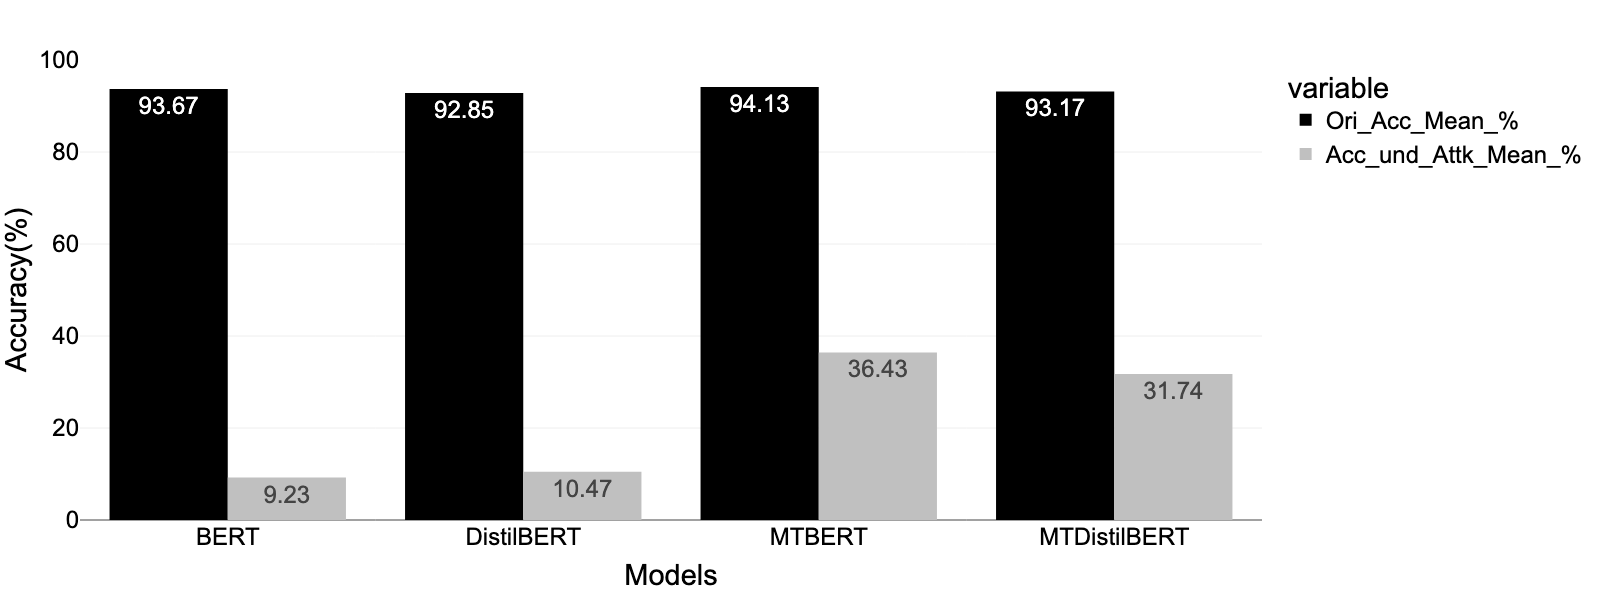
\includegraphics[width=\textwidth]{img/MOAandAUA_Imdb.png}
%%        \caption{IMDB Dataset: Original Accuracy and Accuracy under attack bar plot.}{}
%        \label{fig:imdboa}
%    \end{minipage}
%    \hspace{0.5cm}
%    \begin{minipage}[b]{0.5\linewidth}
%        \centering
%        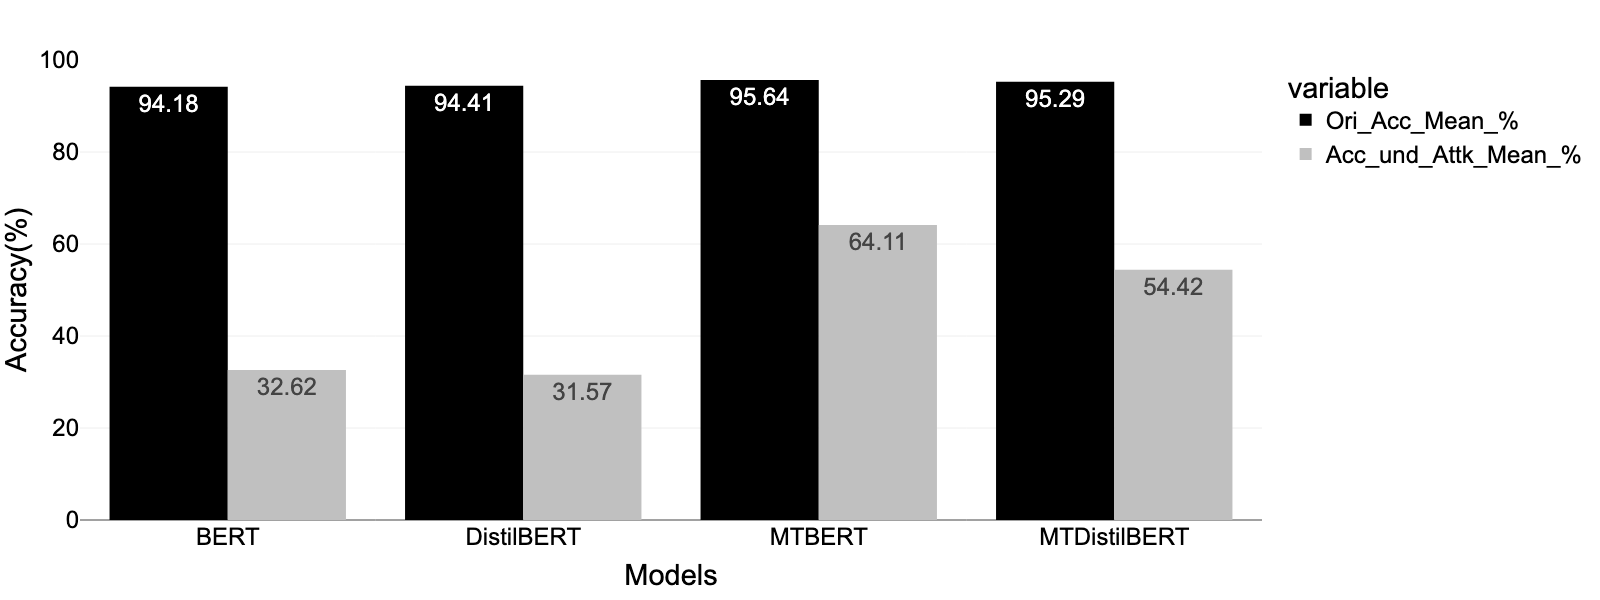
\includegraphics[width=\textwidth]{img/MOAandAUA_fknews}
%%        \caption{Covid-19 fake tweets dataset: }{}
%        \label{fig:fkoa}
%    \end{minipage}
%    \caption[Comparative bar plot of original accuracy and accuracy under attack]{\small Comparative bar plot of original accuracy and accuracy under attack in different dataset. MTBERT showed better performance in both metrics followed by MTDistilBERT. And, highest drop is seen in baseline models (BERT and DistilBERT).}
%    \label{fig:moaandauaimdb}
%\end{figure}
\begin{figure}[H]
    \centering
    \hspace*{2.9em}
    \begin{subfigure}
            \centering
            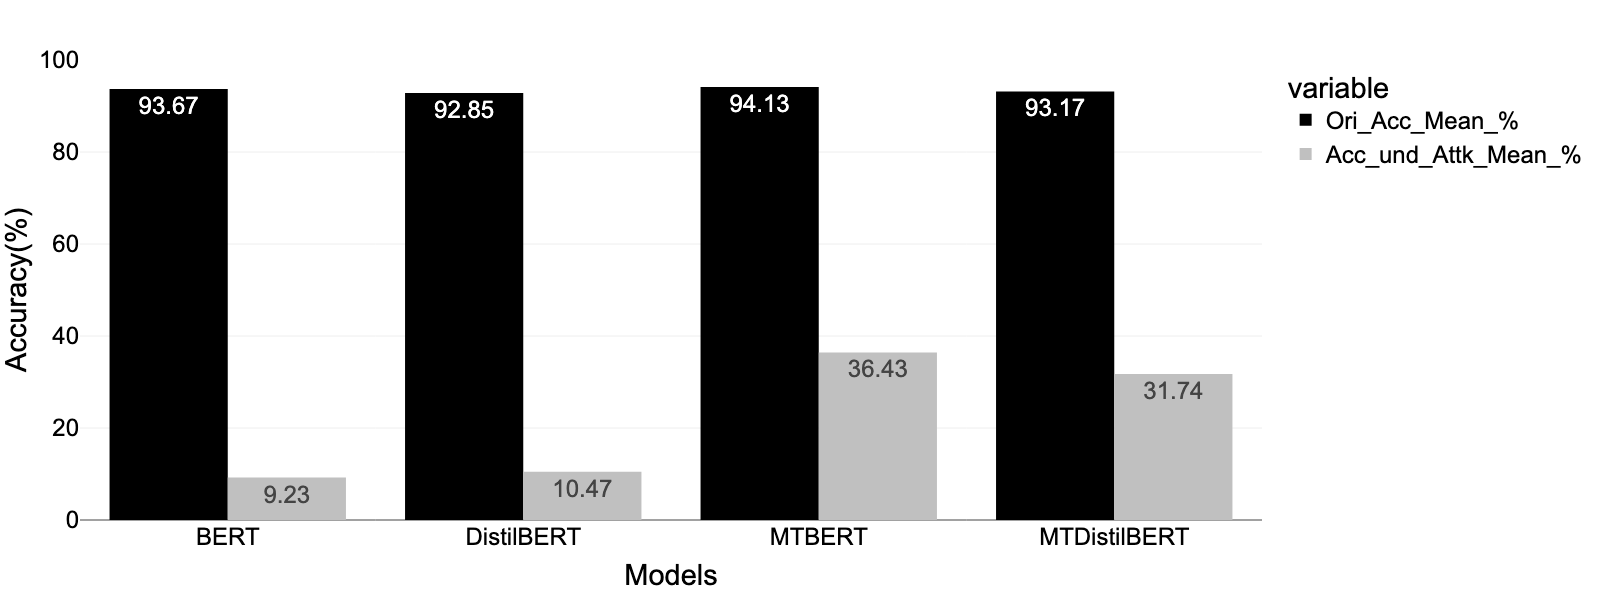
\includegraphics[width=.90\linewidth]{img/MOAandAUA_Imdb.png}
            \caption{IMDB Dataset: Comparative bar plot of between original accuracy and accuracy under attack.}{}
               \label{fig:}
        \end{subfigure}
%    \hspace*{1.8em}
    \begin{subfigure}
            \centering
            \hspace*{2.9em}
            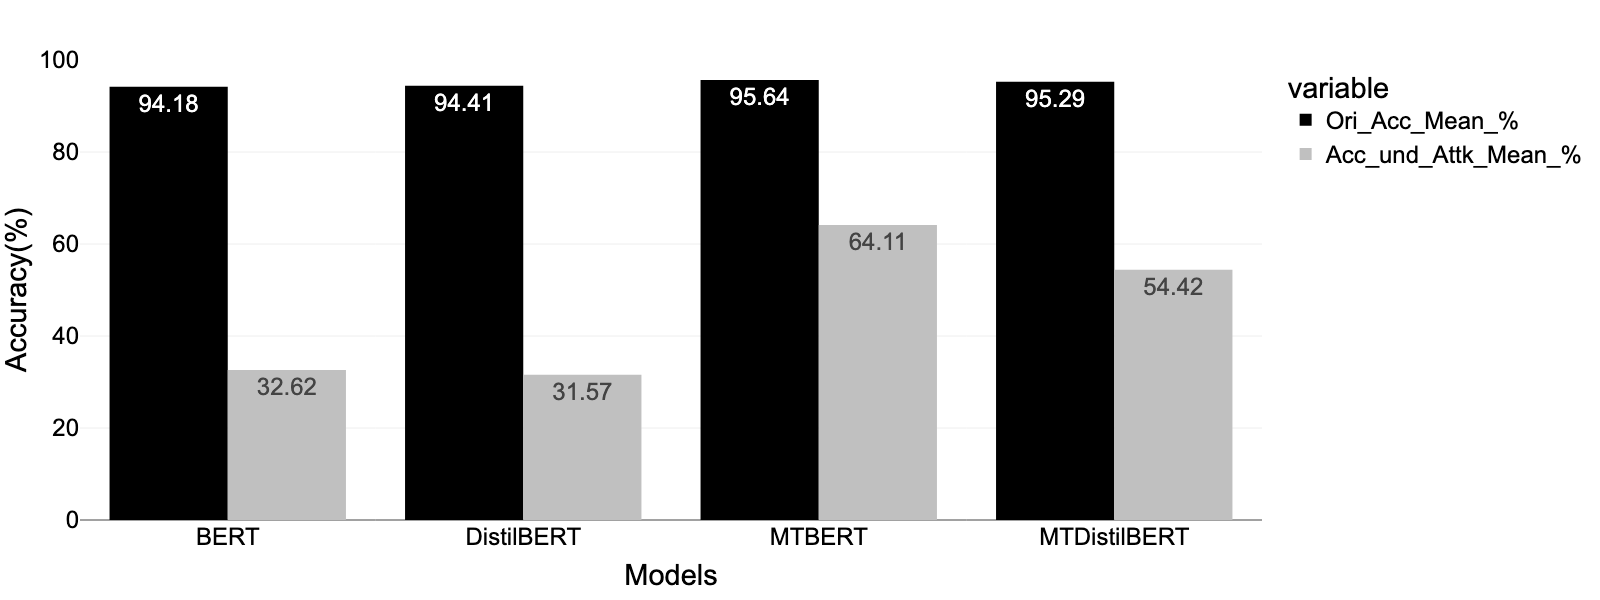
\includegraphics[width=.90\linewidth]{img/MOAandAUA_fknews}
            \caption{Covid-19 fake tweets dataset: Comparative bar plot of between original accuracy and accuracy under attack.}{}
              \label{fig:sub2}
        \end{subfigure}
 \caption[Comparative bar plot between original accuracy and accuracy under attack]{\small Comparative bar plot of original accuracy and accuracy under attack in different datasets. MTBERT showed better performance in both metrics followed by MTDistilBERT. And, the highest drop is observed in baseline models (BERT and DistilBERT).}
  \label{fig:moaandauaimdb}
\end{figure}
\subsection{Number of Queries}
In terms of queries, it is observed that overall MTBERT has a high need for the number of queries to be attacked as shown in bar plot \ref{fig:avgnquebyattackrecipes}.
\begin{figure}[H]
	\centering
%     \hspace*{2.5em}
    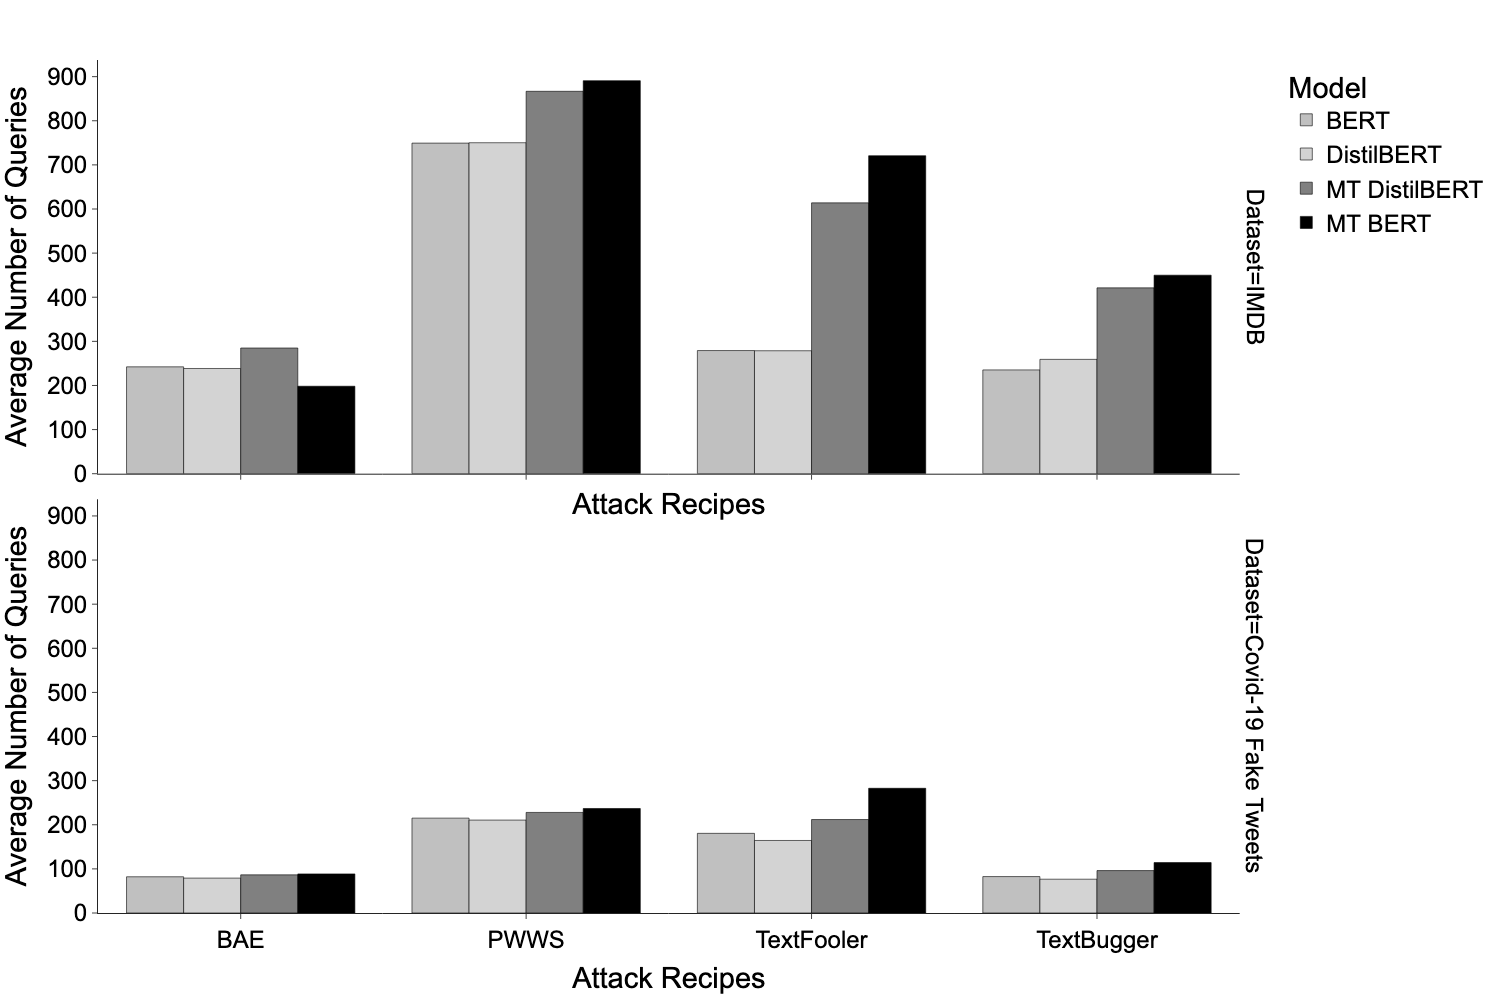
\includegraphics[width=.85\linewidth]{img/AvgNQuebyDataset}
	\caption[Bar plot of the number of queries]{Bar plot of the number of queries w.r.t dataset and attack recipes. PWWS has shown the highest overall number of queries requirement followed by TextFooler.  And, dependencies w.r.t to text length can also be observed in this plot.}
	\label{fig:avgnquebyattackrecipes}
\end{figure}
\begin{figure}[H]
    \centering
    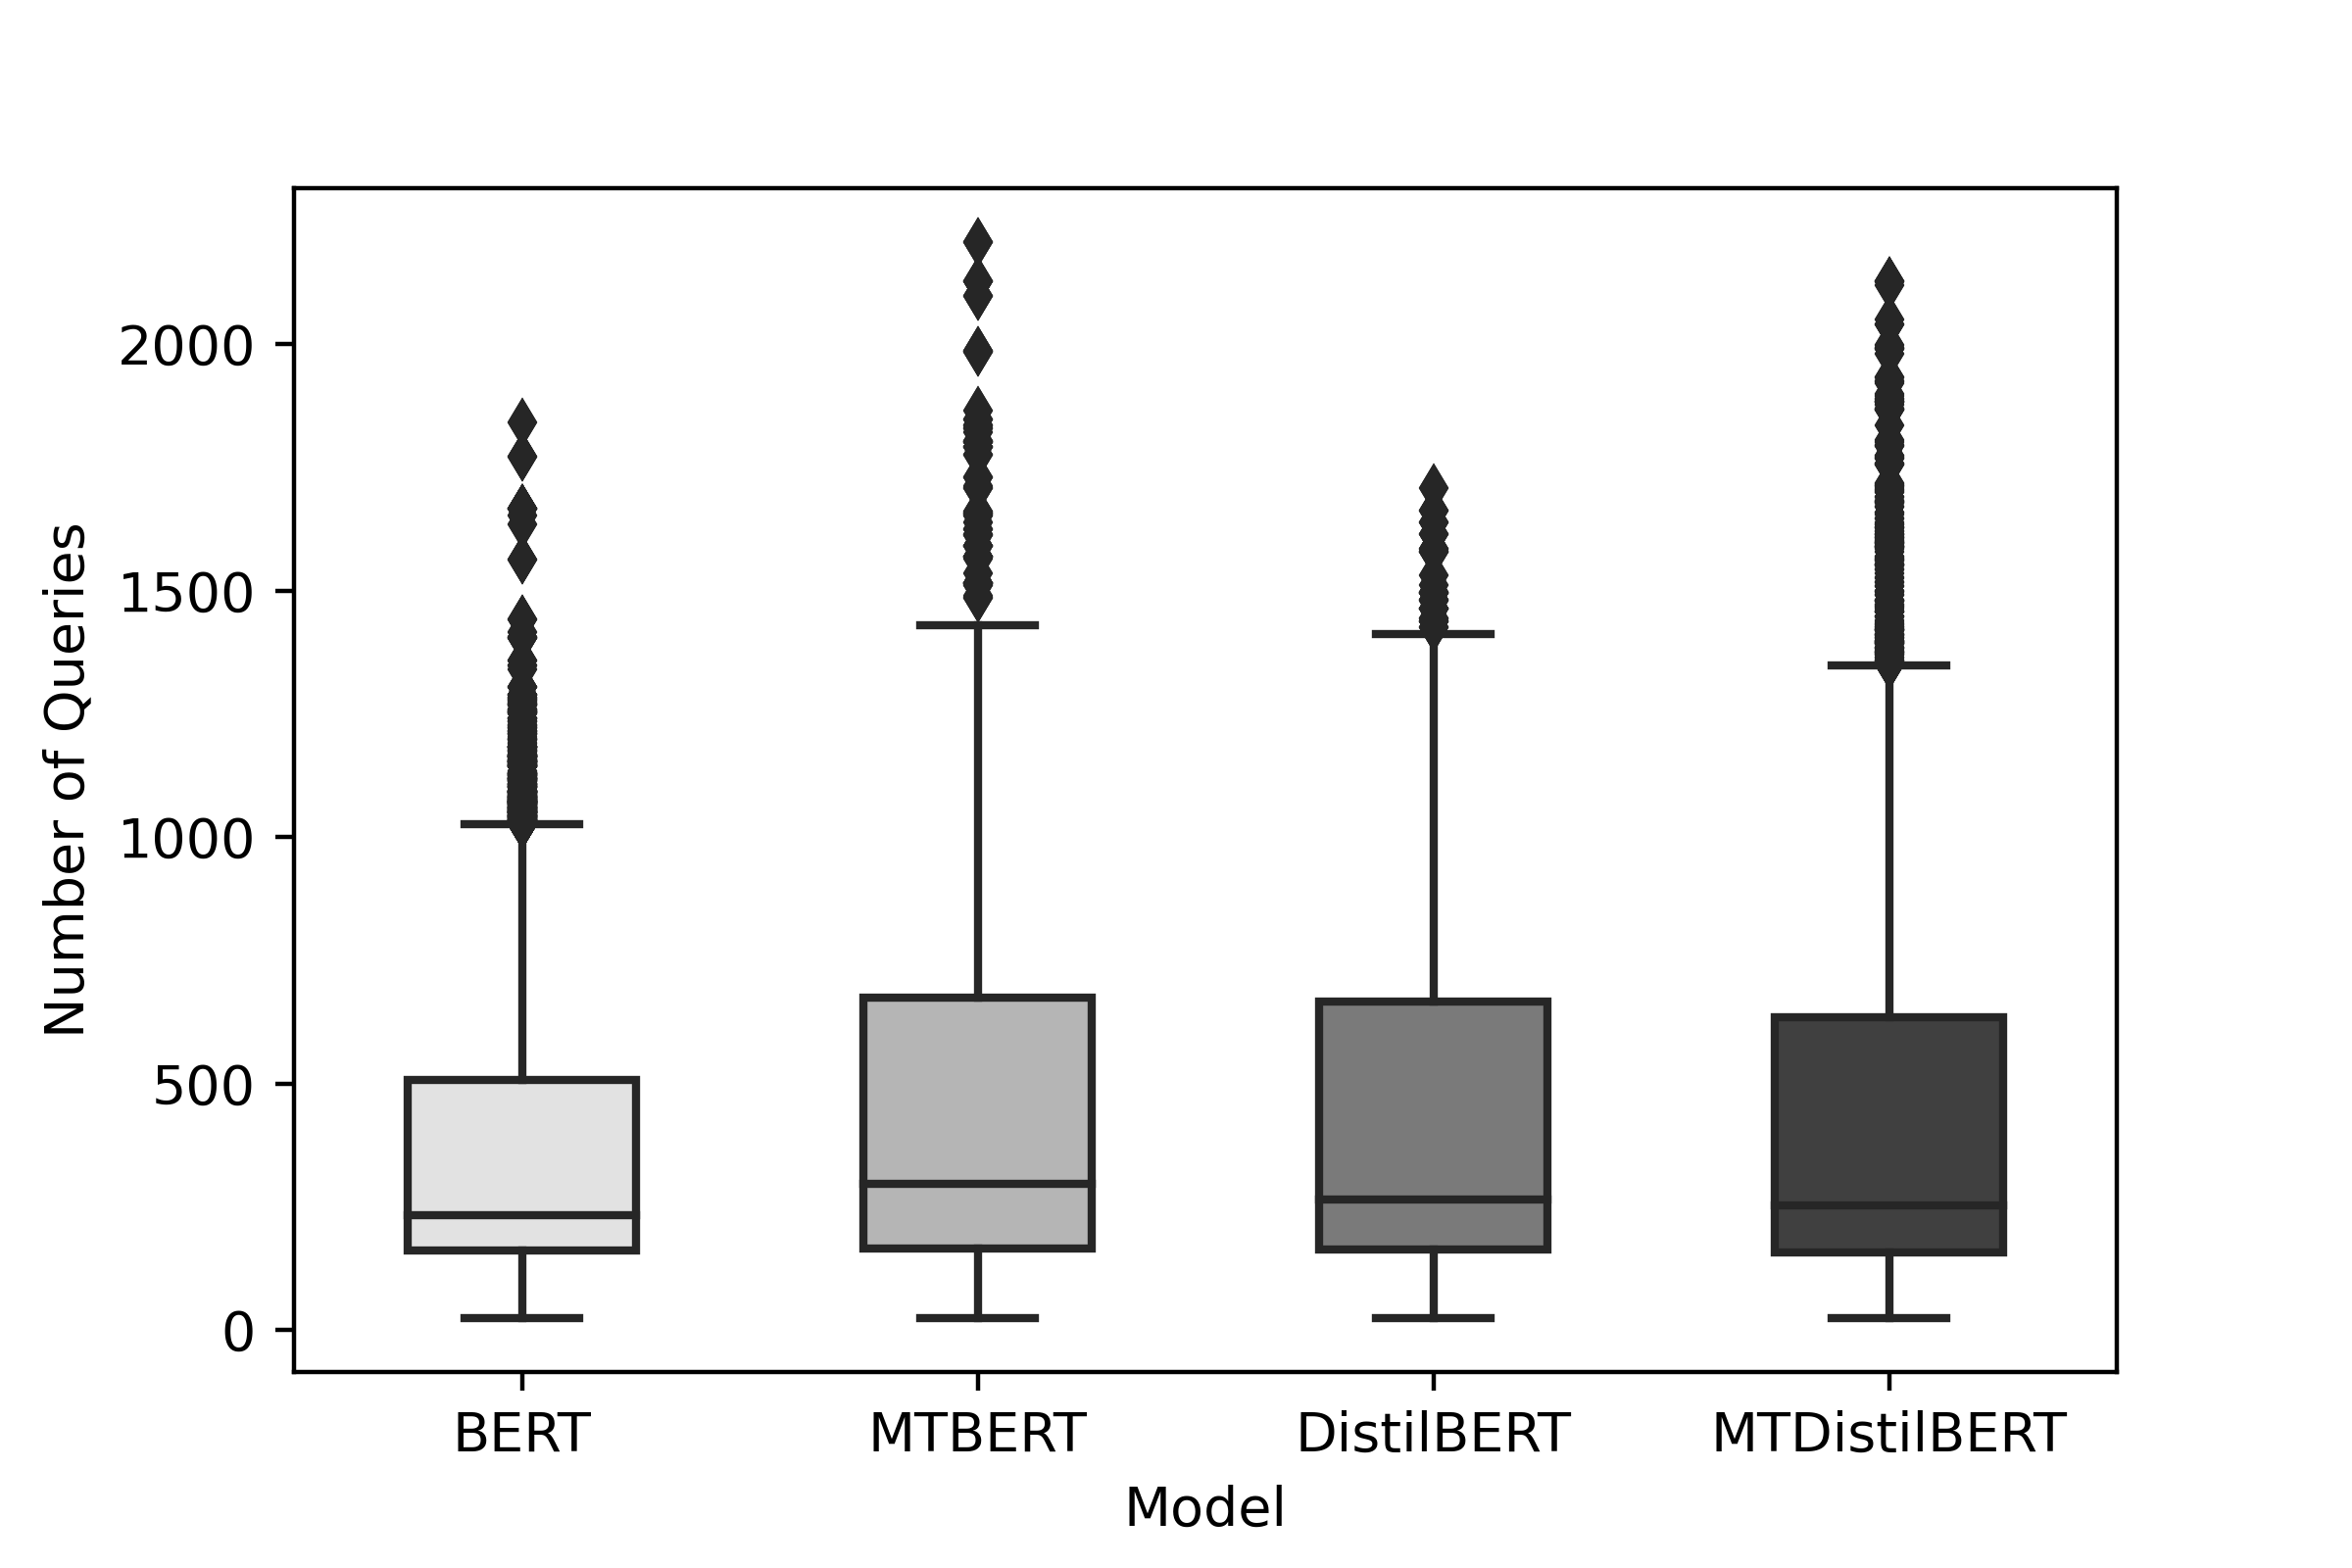
\includegraphics[width=0.70\linewidth]{img/NumQueriesDist_box_IMDB.png}
    \caption[Box plot of the number of queries.]{ Box plot of the number of queries. The proposed approach models are comparatively broader and showed greater values for outliers than baseline models. This particular box plot is based on the IMDB dataset and only successful attacks are considered.}
    \label{fig:numofqueriesdist}
\end{figure}
 As shown in the box plot \ref{fig:numofqueriesdist}, the interquartile range of the MTBERT and MTDistilBERT model is comparatively broader than any other model and has also shown incident crossing 2000 queries. \\
If we compare the performances of attack recipes, BAE attacks have shown the lowest requirements for queries, followed by TextBugger, however, it is the least effective in attacking. PWWS requires a significantly higher number of queries followed by TextFooler and is also found to be more effective in attacks. \\
Furthermore, PWWS and TextFooler attack recipes are dependent on the text length considering differences in queries of both the dataset shown in the figure \ref{fig:avgnquebyattackrecipes}. In the TextFooler attack recipe, the difference between proposed and baseline queries also increases with respect to the text length which also shows its effectiveness depends on text length. The distribution of number of queries is shown in figure \ref{fig:Queries_distribution_fk} and \ref{fig:Queries_distribution_imdb} in appendix \ref{chapter:appendix}.
\subsection{Perturbation Score}
Intuitively, the perturbation score that is predicted probability under attack in other term confidence score were logged during experiments.  Because, it answers the question about  resilience demonstrated by proposed and baselines models in terms of confidence in prediction. 
\begin{figure}[H]
    \centering
    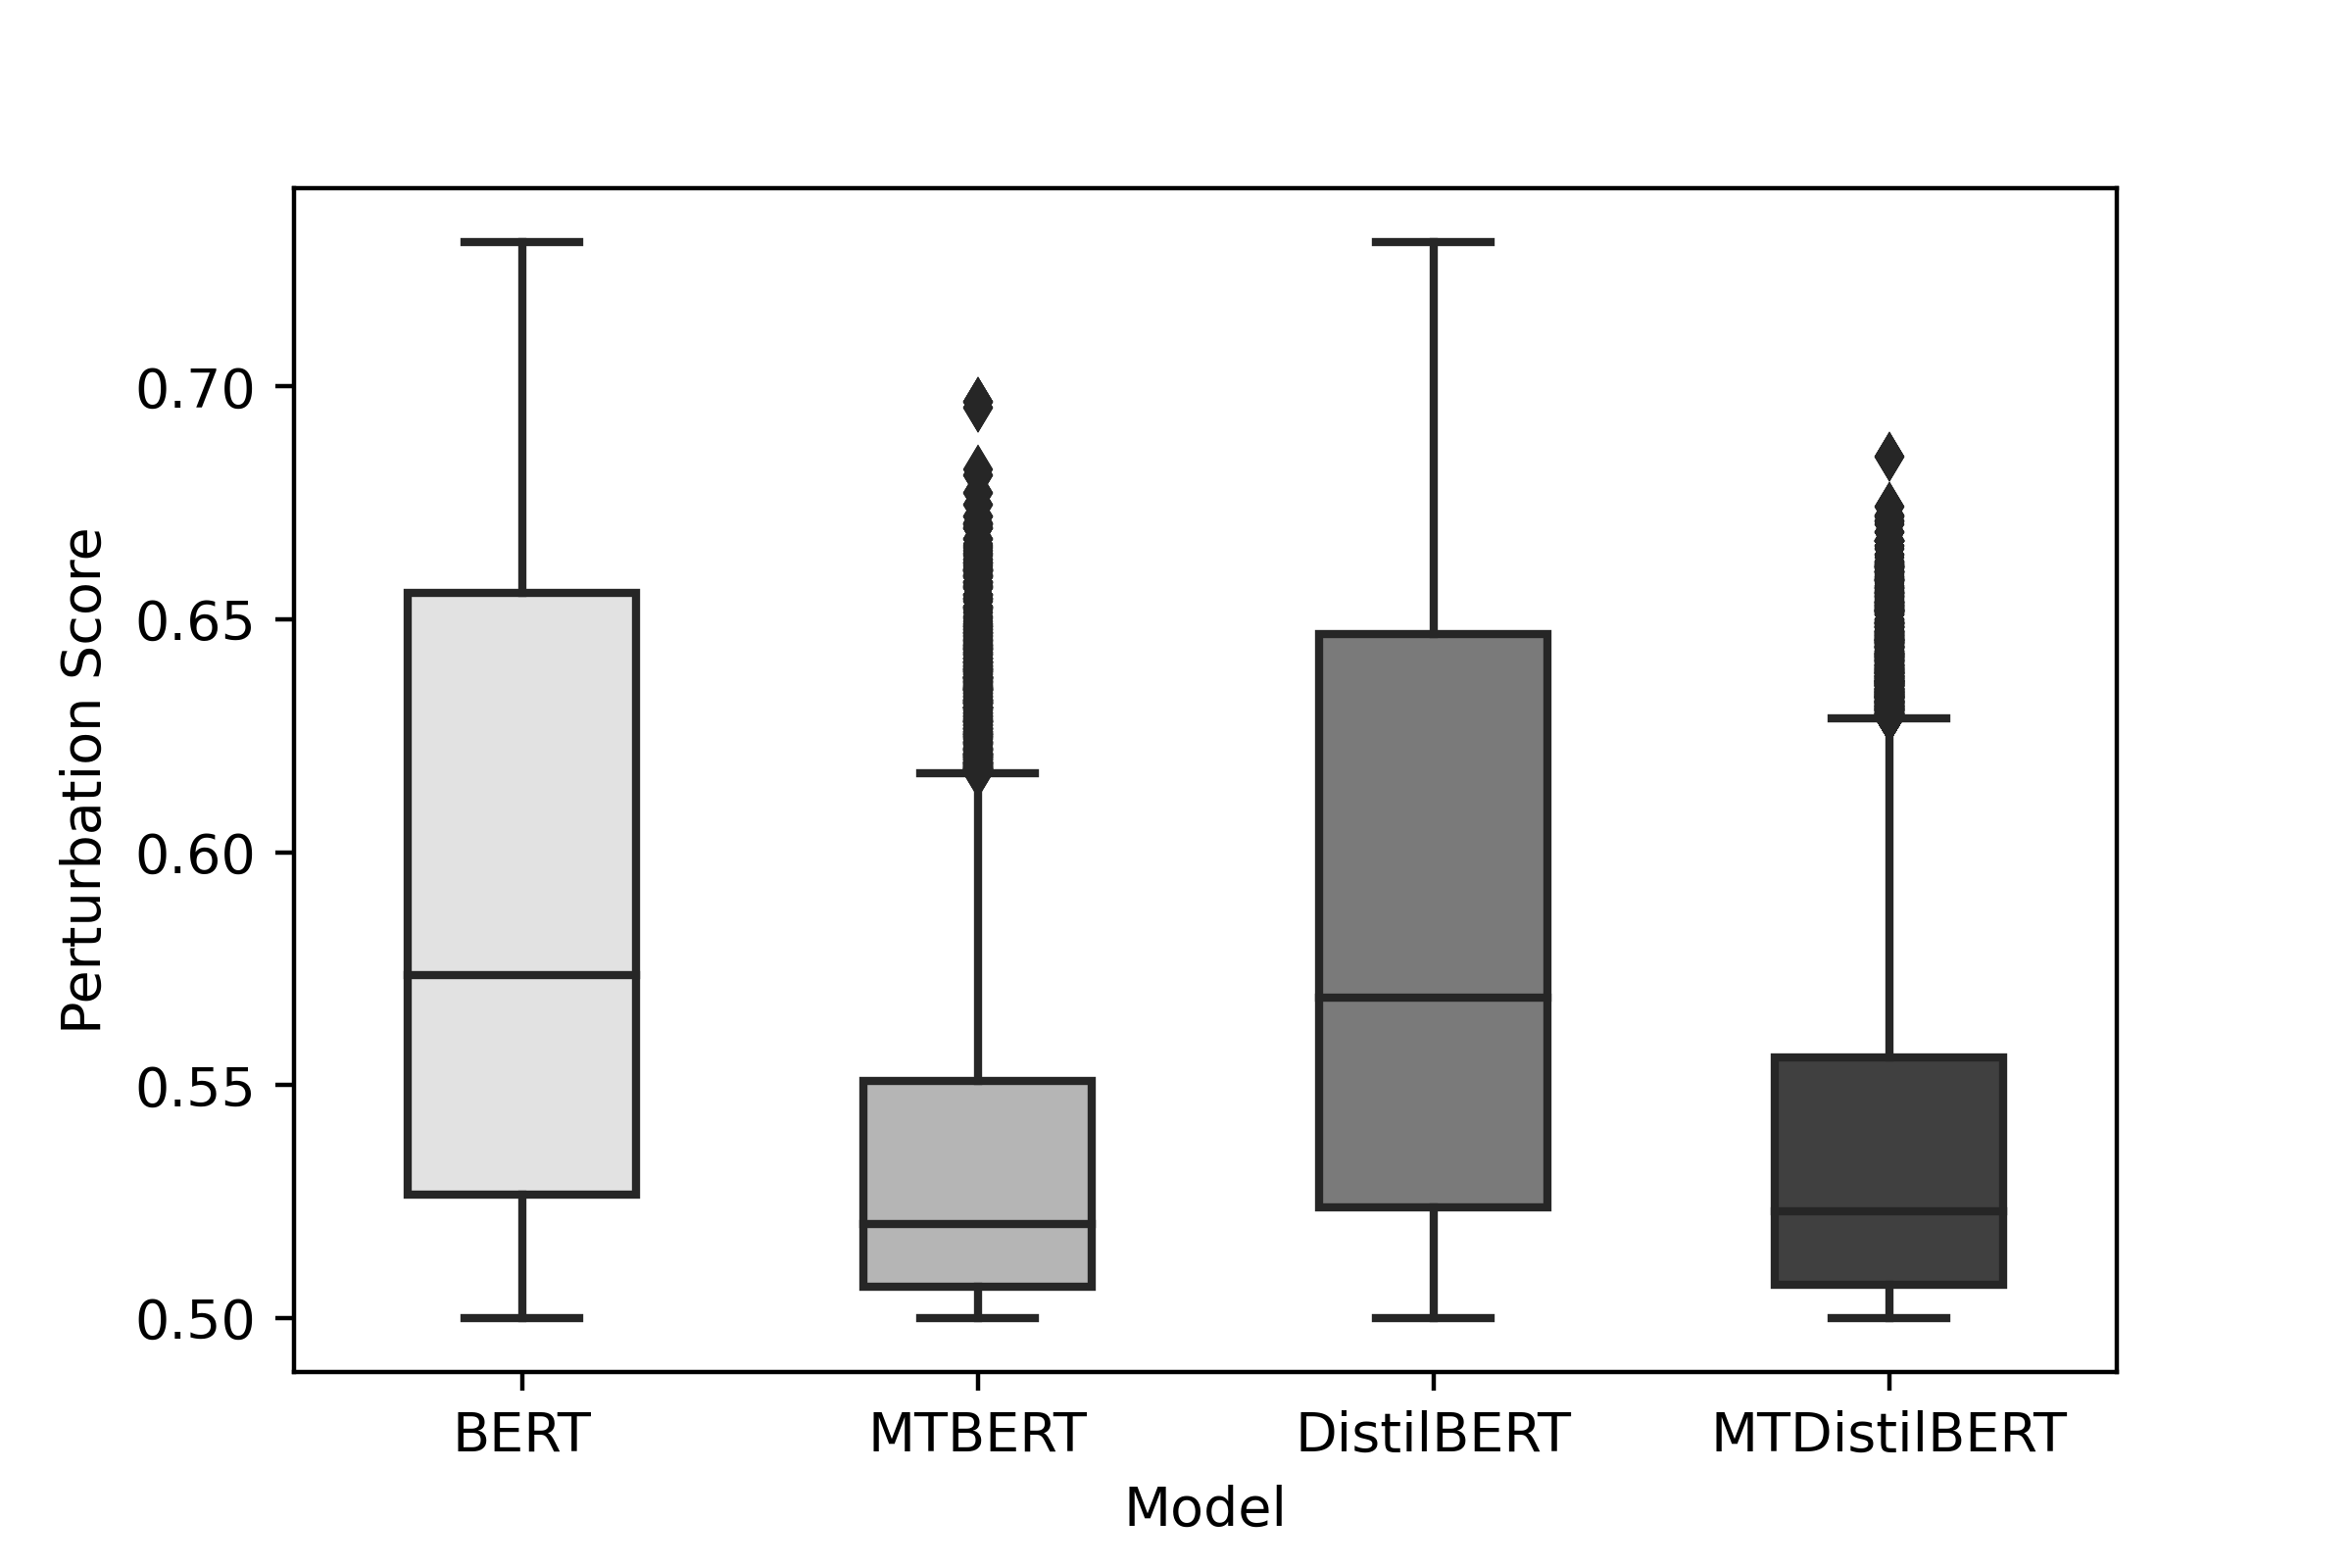
\includegraphics[width=.70\linewidth]{img/PertScoreDist}
    \caption[Box plot of perturbation score]{\small Box plot of perturbation score. MTBERT model has managed attacks confidence score in the leaner interquartile range and does not cross 0.70 which is a significant improvement over BERT.}
    \label{fig:pertscoredist}
\end{figure}
As shown in the figure \ref{fig:pertscoredist}, a remarkable improvement is being observed in the proposed model  with respect to the baseline model and the perturbation score distribution of the proposed approach model is comparatively more left-shifted than baseline models is shown in figure \ref{fig:PerturbationScore_Dist_IMDB} and \ref{fig:PerturbationScore_Dist_fakenews} in appendix \ref{chapter:appendix}. \\
The proposed approach model does not let attack recipes go beyond a particular limit i.e. 0.70, however, baseline models are more uniform and show less resilience.  The range of the MTBERT model is 0.50 to 0.55, but for the BERT model, it is 0.50 to 0.66, which is a significant improvement in the model.
The distribution of perturbation score is shown in figure \ref{fig:PerturbationScore_Dist_IMDB} and \ref{fig:PerturbationScore_Dist_fakenews} in appendix \ref{chapter:appendix}.
\subsection{Word Perturbation}
To understand the robustness of models with respect to word perturbation, the difference is less significant in between models as shown in the figure \ref{fig:avgpertbyattackrecipes}. However, in the Covid-19 fake tweets dataset, the average word perturbation required by proposed models is higher, but, exactly the opposite in the IMDB dataset.
\begin{figure}[H]
    \centering
     \hspace*{2.5em}
    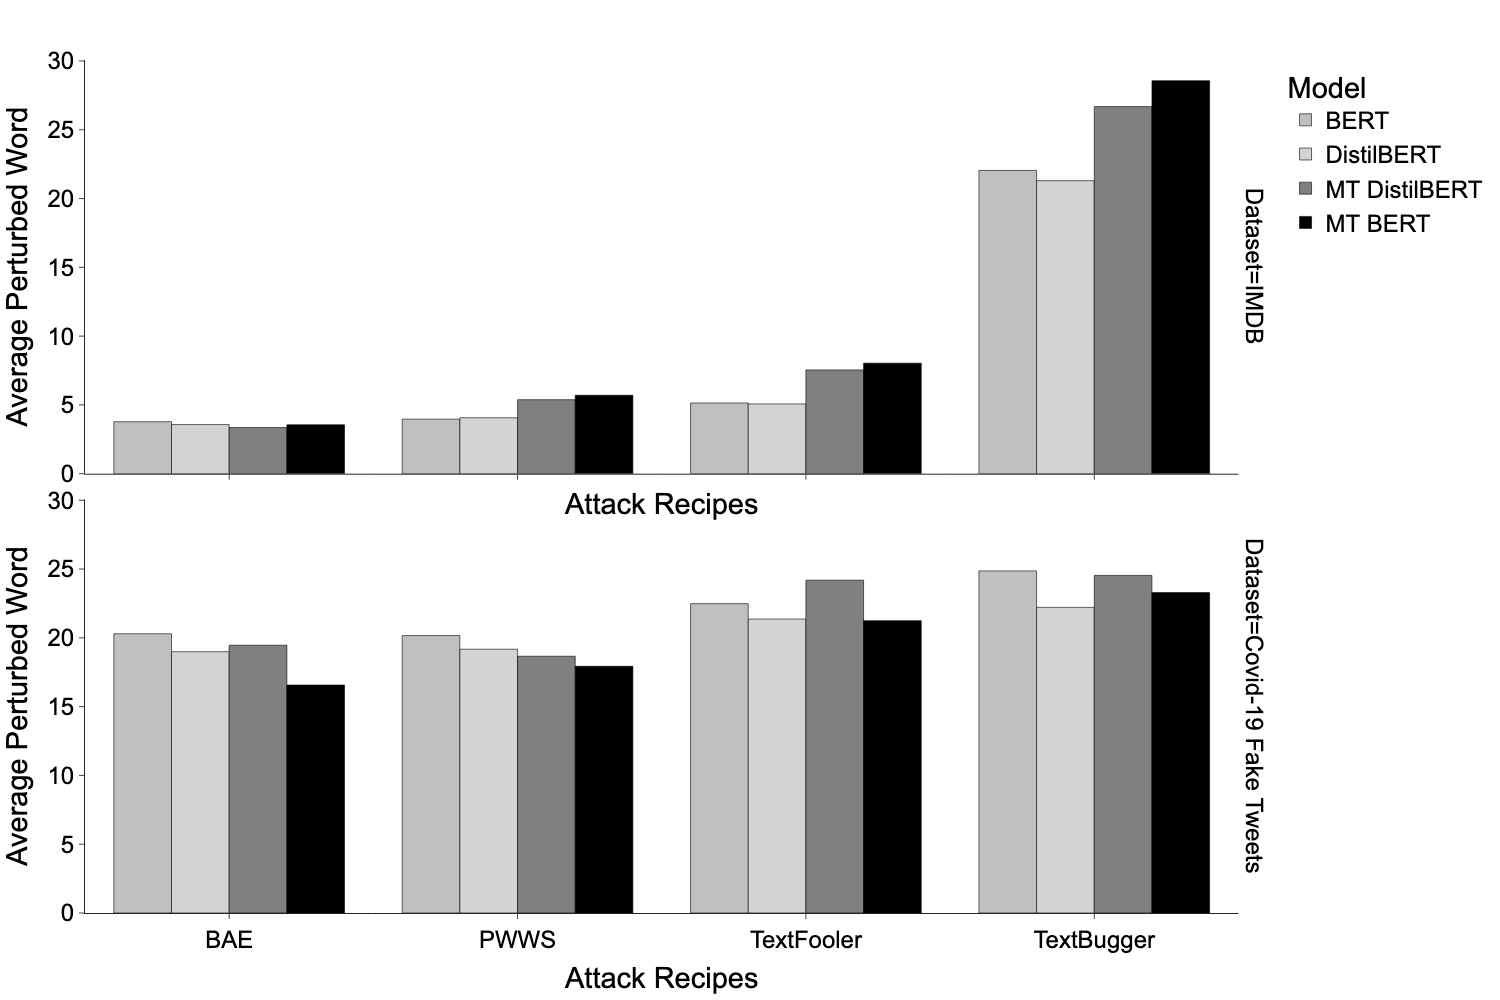
\includegraphics[width=0.9\linewidth]{img/AvgPertByDataset}
    \caption[Bar plot of word perturbation rate]{Bar plot of word perturbation as per datasets and attack recipes. TextBugger has shown the highest word perturbation in both datasets and also shown less difference between both datasets. However, BAE has lower word perturbation followed by the PWWS attack recipe. Covid-19 fake tweets dataset has shown significantly higher word perturbation requirements.  }
    \label{fig:avgpertbyattackrecipes}
\end{figure}
 It is quite clear that longer text requires comparatively lower  word perturbation which also make sense. But, surprisingly, TextBugger has shown the same perturbation rate and is least affected by text length. However,  TextBugger requires a greater number of words perturbed than TextFooler. BAE required the lowest number of perturbations, followed by PWWS.
\subsection{Attack Success Rate}
\label{subsection:attacksuccessrate}
The attack success rate is a complementary metric of accuracy under attack which helps in determining the effectiveness of  attack recipes.
As shown in the bar plot \ref{fig:attacksuccessrate}, the TextFooler  is the most effective attack recipe, followed by PWWS  attack recipe. On the other hand, the BAE  has exhibited the worst performance, followed by TextBugger. \\
In addition, all attack recipes have been more successful in the IMDB dataset in contrast to other dataset. This indicates their relationship with text length or access to a wide vocabulary range. Furthermore, all attack recipes were least effective against proposed approach fine-tuned models and most effective against conventionally fine-tuned models.
\begin{figure}[H]
    \centering
    %    \hspace*{2.5em}
    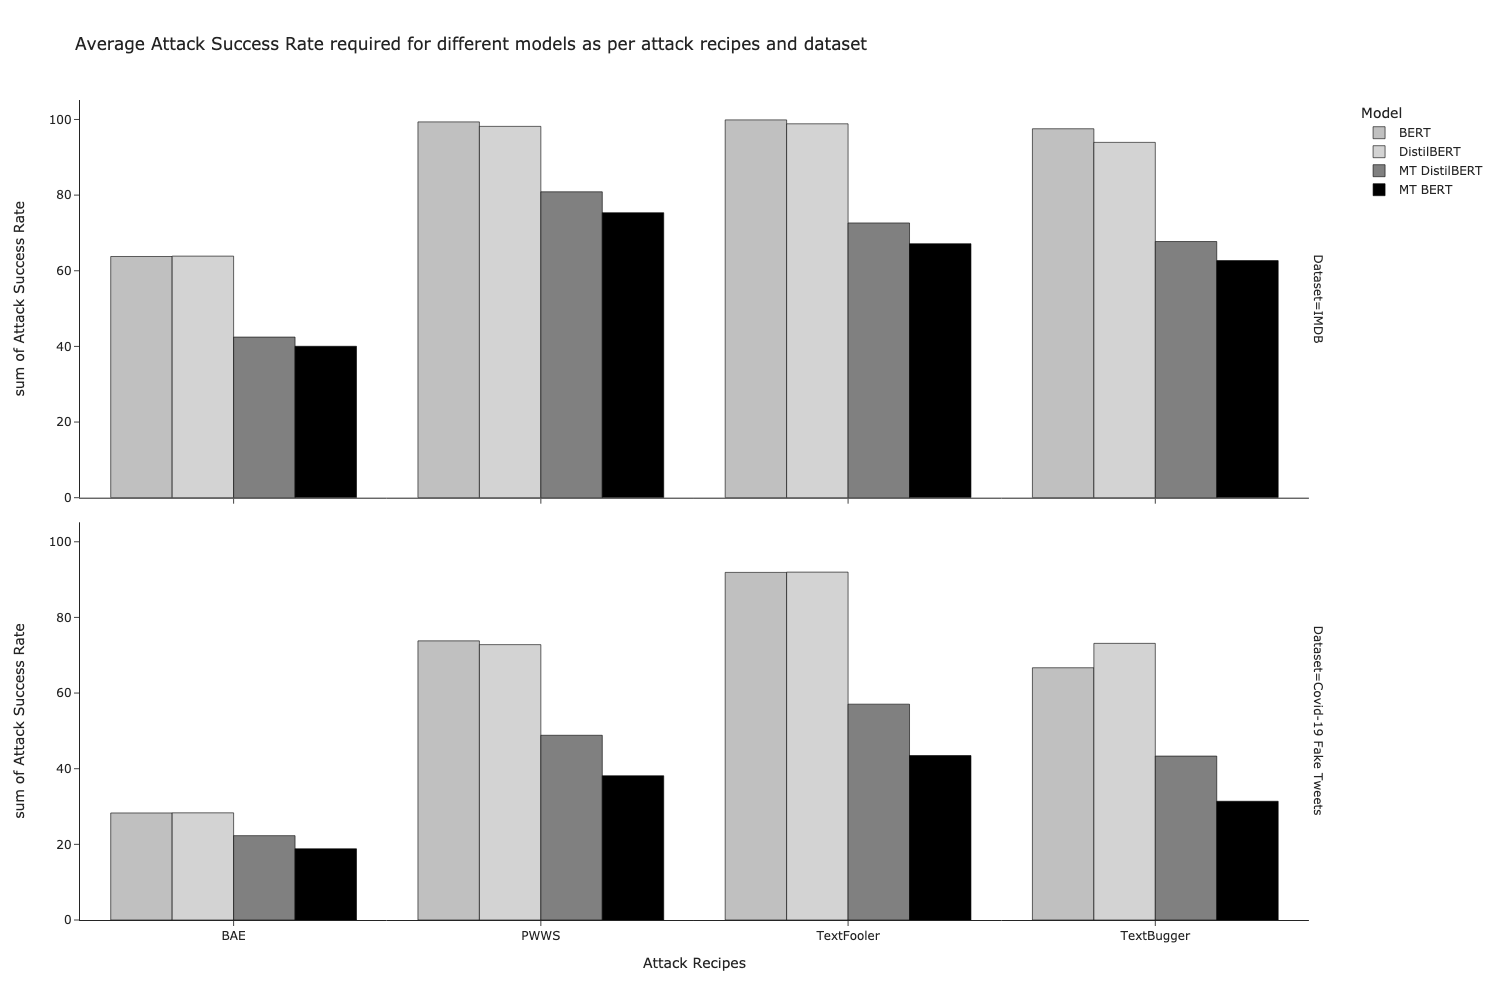
\includegraphics[width=.9\linewidth]{img/attack_success_rate.png}
    \caption[Bar plot of attack success rate]{Bar plot of attack success rate. The TextFooler attack recipe observed to be most effective at attacking the language models followed by PWWS. On the other hand, BAE has been least effective, followed by TextBugger. Furthermore, language models fine-tuned using the proposed approach show the lowest attack success rate. }
    \label{fig:attacksuccessrate}
\end{figure}
Overall, the model fine-tuned with the proposed approach has shown a significant improvement over conventional method of fine-tuning in that MTBERT has demonstrated maximum robustness. In the experiment, it is also observed that compact model i.e. DistilBERT created using knowledge distillation are performing comparatively less to its base model i.e. BERT. The most prominent explanation would be the loss of information during distillation process. Furthermore, TextFooler and PWWS  appeared to be most successful attacks recipes. 
%\begin{figure}
%    \centering
%    \begin{minipage}{.5\textwidth}
%        \centering
%        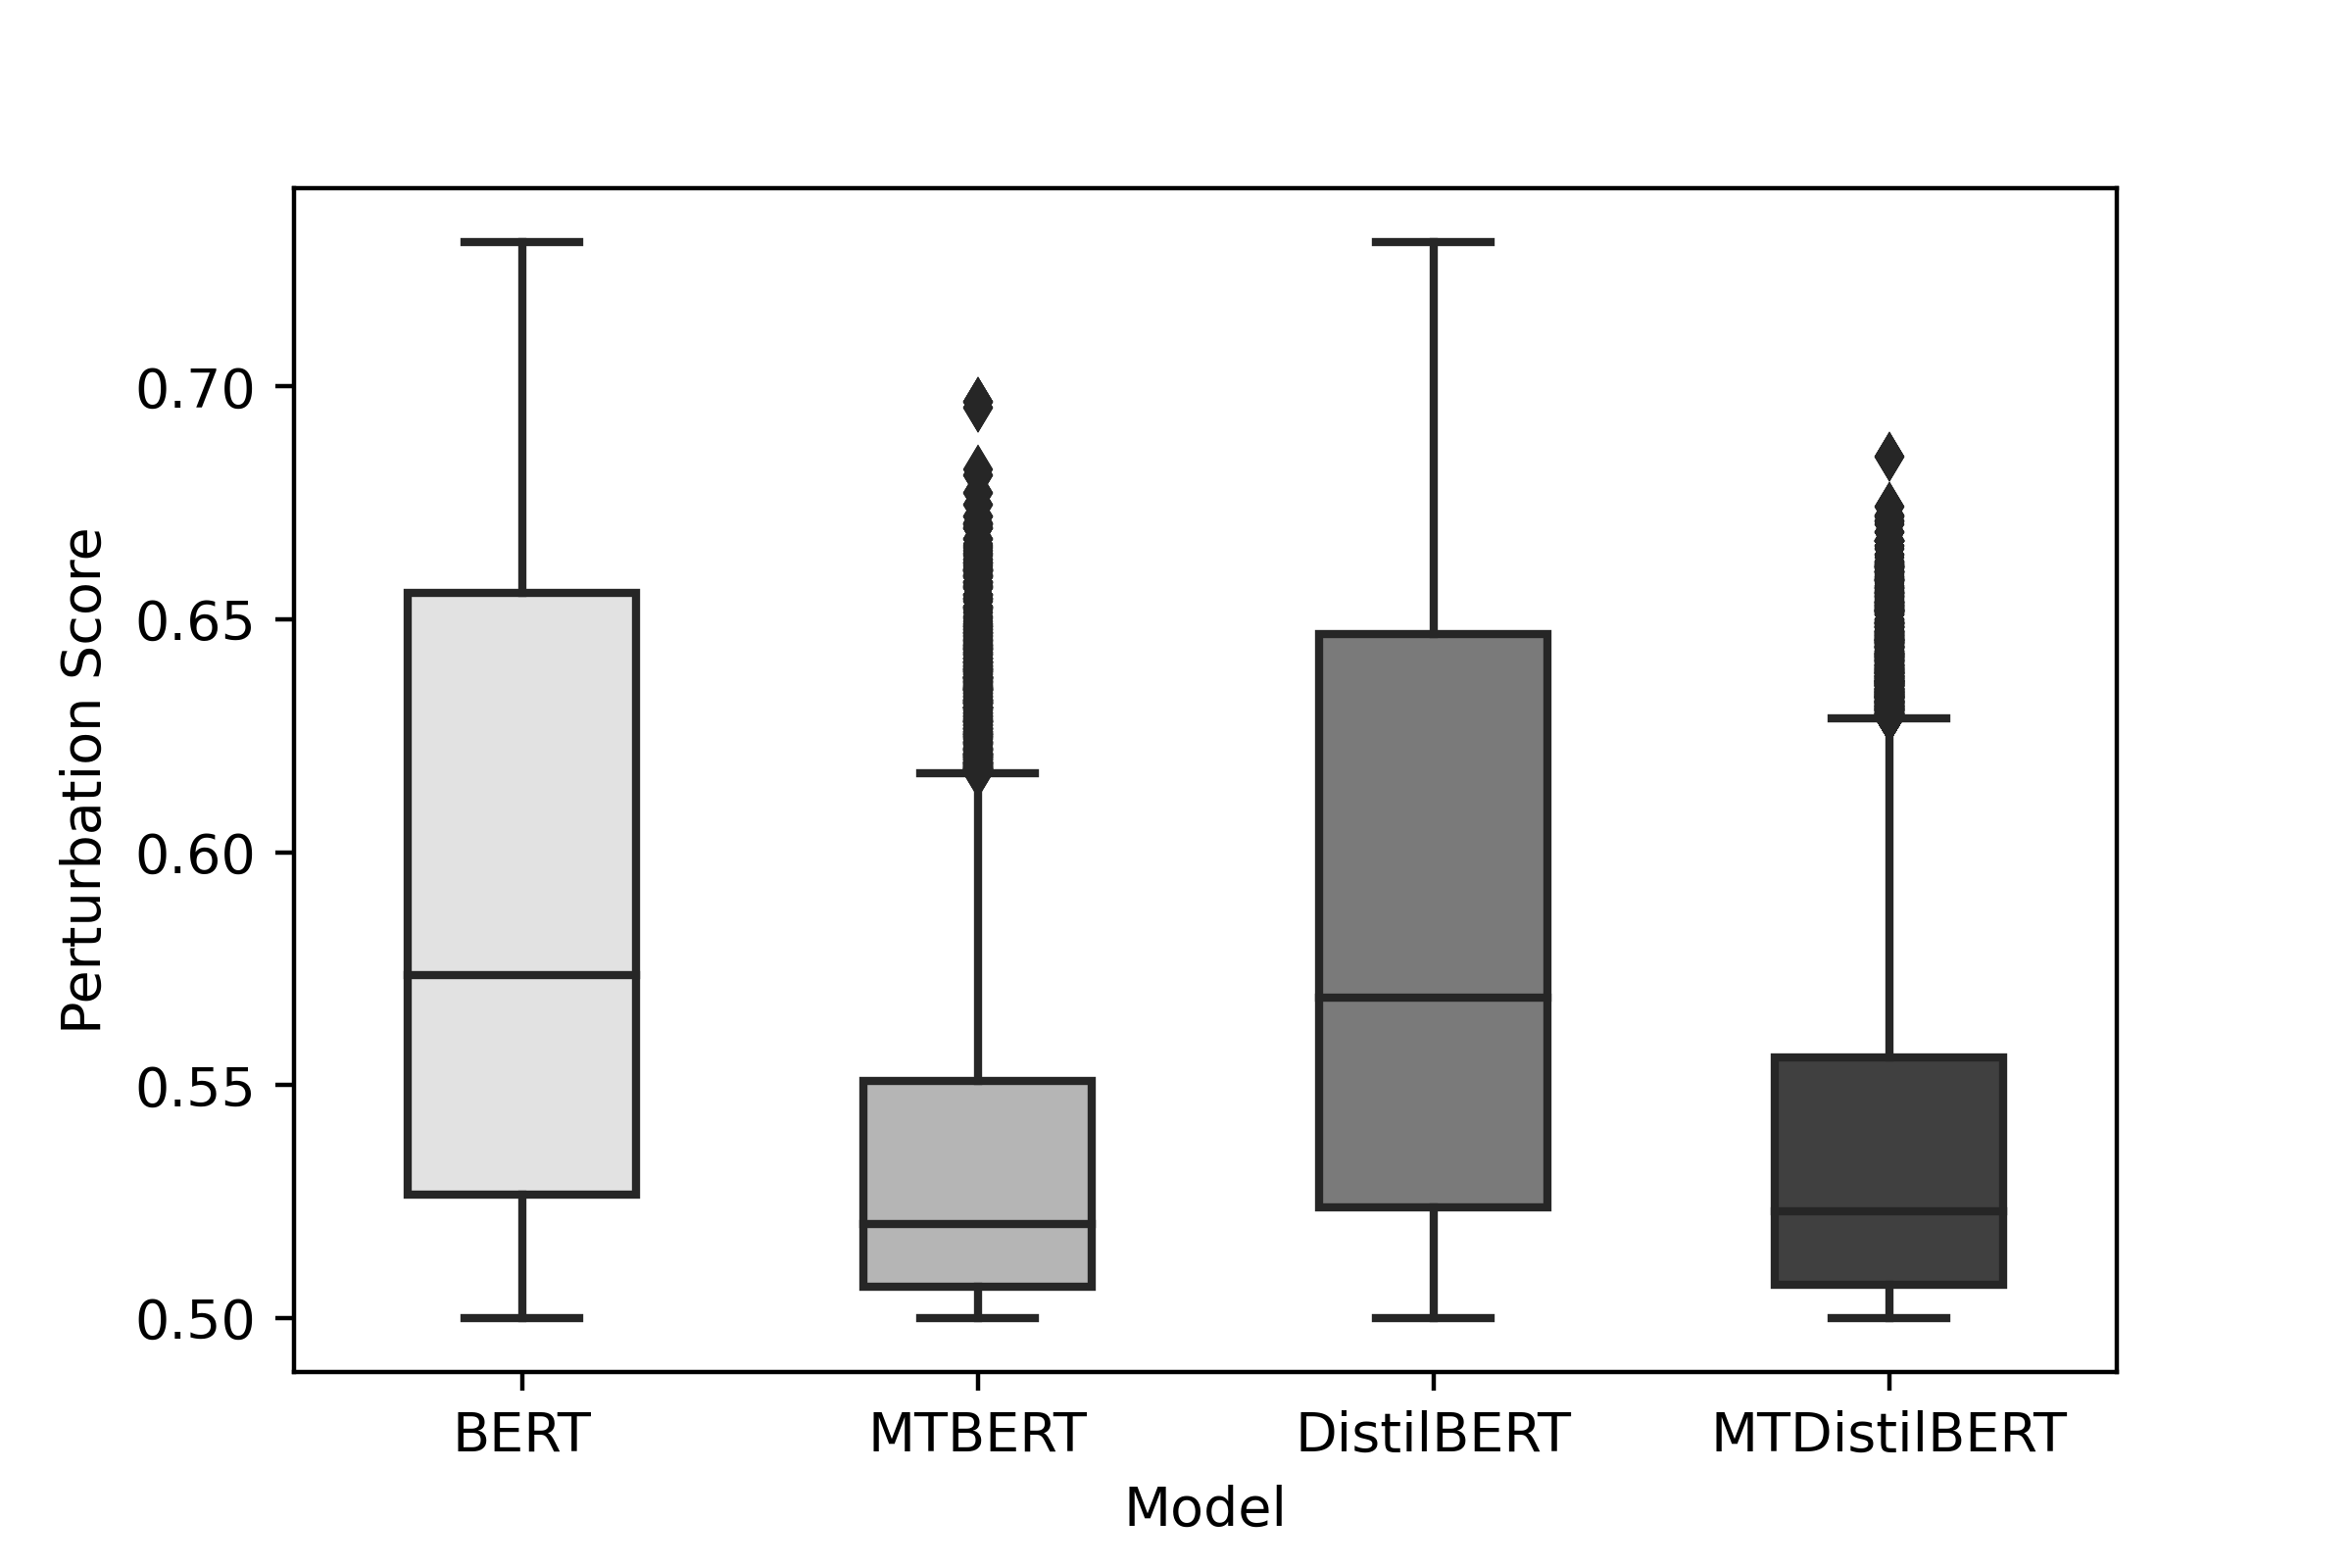
\includegraphics[width=.6\linewidth]{img/PertScoreDist.png}
%        \captionof{figure}{A figure}
%        \label{fig:test1}
%    \end{minipage}%
%    \begin{minipage}{.5\textwidth}
%        \centering
%        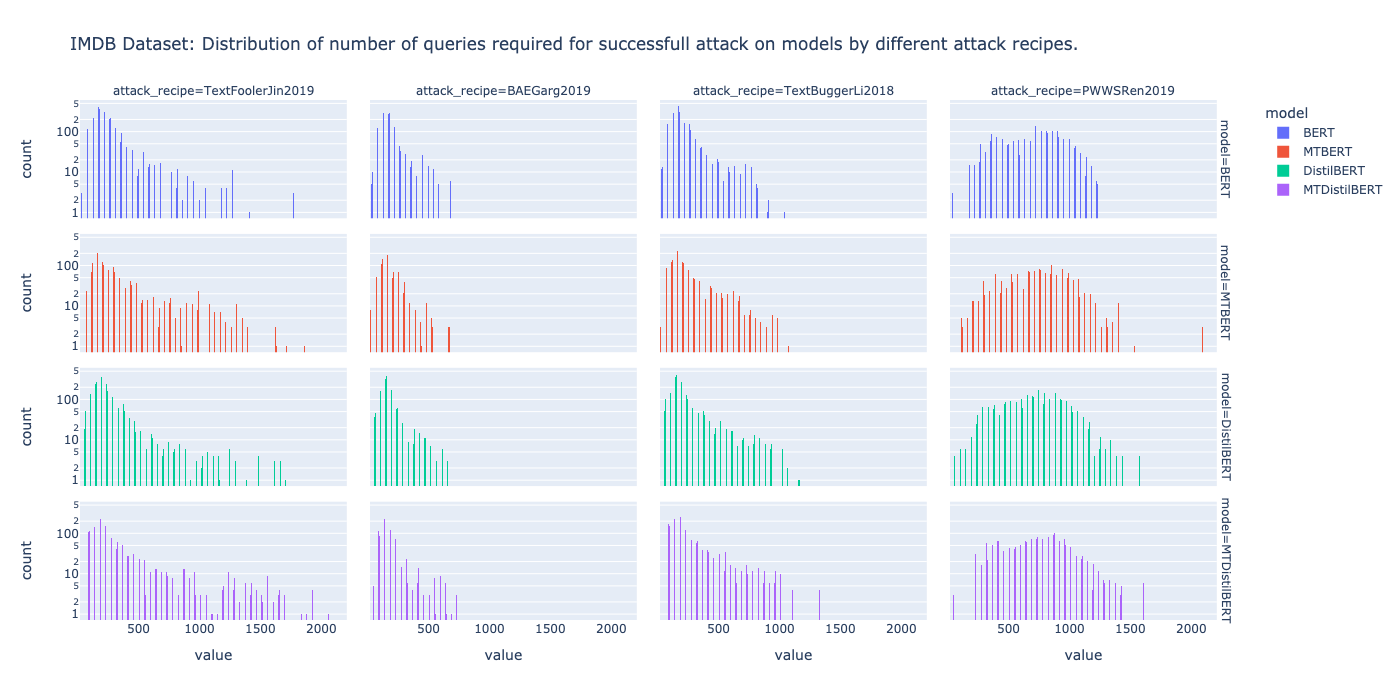
\includegraphics[width=.6\linewidth]{img/NumQueriesDist_IMDB.png}
%        \captionof{figure}{Another figure}
%        \label{fig:test2}
%    \end{minipage}
%\end{figure}

%\begin{table}[h!]
%    \centering
%    \hspace*{-0.7em}
%    \resizebox{1.0\textwidth}{!}{
%        \begin{tabular}{llrrrrrrrr}
%            \toprule
%            {} &         model &     count &  mean &  std &  min &  25\% &  50\% &  75\% &  max \\
%            \midrule
%            0 &          BERT & 38,507.00 &  0.59 & 0.07 & 0.50 & 0.53 & 0.57 & 0.66 & 0.73 \\
%            1 &    DistilBERT & 47,222.00 &  0.59 & 0.07 & 0.50 & 0.52 & 0.57 & 0.64 & 0.73 \\
%            2 &        MTBERT & 22,262.00 &  0.53 & 0.04 & 0.50 & 0.51 & 0.52 & 0.55 & 0.70 \\
%            3 &  MTDistilBERT & 32,012.00 &  0.54 & 0.04 & 0.50 & 0.51 & 0.52 & 0.56 & 0.67 \\
%            \bottomrule
%        \end{tabular}
%  }
%    \caption{Perturbation score table }{Perturbation score descriptive statistics of  successful attacks combining both dataset. Proposed model has shown significant improvement over baseline model. 
%        And, mostly in limited in range 0.53-0.70 and 75 \% of attacks score is under 0.55 a sign of robustness.}
%    \label{table:perturbationscore}
%\end{table}
\newpage
\section{Discussion on Research Question}
The objective of this master thesis was to conduct experiment and investigate the research question: \\
%\emph{Is it possible to enhance robustness and generalization of language models with proposed mean teacher semi-supervised fine-tuning and employing prominent adversarial unlabelled data during training, compared to a conventional approach?}\\

\emph{Is the proposed mean teacher semi-supervised fine-tuning and the use of prominent adversarial unlabelled data an effective method to improve the robustness of language models, specifically with regard to accuracy under attack without compromising the original accuracy in contrast to the conventional fine-tuning approach?}\\

This experiment hypothesized that the proposed mean teacher semi-supervised approach and use of prominent adversarial unlabelled data will produce a comparatively robust language model in terms of metrics such as accuracy under attack, queries required, rate of word perturbation, and confidence score without compromising generalization. And, it  was expected that the mean teacher language model would outperform the traditional fine-tuned model, and same has been confirmed throughout the experiment.\\
According to the findings, the proposed approach has demonstrated notable increase in generalization and a significant improvement in accuracy under attacks. The language model produced using proposed approach requires higher word perturbation and queries to get attacked. Furthermore, the proposed fine-tuned model has shown remarkable improvements in terms of confidence score, i.e., attack recipes are not able to misclassify the prediction with higher confidence.\\
In the proposed semi-supervised approach, two key techniques are expected to account for observed behaviour: 1) Data Augmentation, and 2) Exponential Moving Average (EMA). However, this research does not attempt to quantify the impact of these strategies on observed behaviour. 
\subsection{Data-Augmentation}
During training, data augmentation incorporates numerous additional words as noise, resulting in models learning a bigger word representation and also regularize the model at the same time. This, however, is the most basic explanation and only using noisy data during training does not guarantee improvement. \\
Englesson \textit{et al.} \cite{englesson_consistency_2021} claimed that models trained on noisy data perform worse than models trained on clean data, and that the performance of models trained on noisy data worsens as the noise ratio rises. However, introducing a separate loss function to deal with noisy data during training can improve model performance and robustness significantly and it is referred as consistency regularization.  Hence, in the proposed approach of fine-tuning consistency loss was included.\\
Both gradient-based techniques \cite{miyato_virtual_2018} and the proposed methodology exploit the concept of consistency regularization. Furthermore, the suggested strategy also backs up the conclusions of Belinkov \textit{et al.} \cite{belinkov_synthetic_2018} study, which indicate that including noisy data during training improves model robustness. This answers the question of whether language models trained on noisy data with a loss function termed consistency loss can increase generalization and robustness.\\
In conclusion, if appropriate data augmentation procedures are implemented in semi-supervised fine-tuning methodology, better predicting and robust language models can be achieved.
\subsection{Exponential Moving Average}
In another case, it is commonly known that ensemble technique can outperform a single machine learning models. Laine et al. \cite{laine_temporal_2017} exploited this idea and applied it at training level, averaging the prediction of single network over multiple different training epochs and augmentation conditions. Their study found that such type of ensemble technique can also lead to a stronger predictor. Later,  Tarvainen \textit{et al.} \cite{tarvainen_mean_2018} claimed and demonstrated that, averaging model weights throughout training can also lead to a much better predictor instead averaging model prediction. \\
Their research was based on the findings of Polyak \textit{et al.} \cite{polyak_acceleration_1992}, who found that averaging weights over time provides a more accurate model than using final weights directly. Therefore, the teacher model better since it was an average of consecutive student models. \\
This thesis provides experimental evidence supporting all the above mentioned studies, and claiming that the language model created using average weight assignment and data augmentation creates a comparatively better and more robust model when it comes to defending against adversarial attacks.\\
The experiment's transferability to other language models is partially demonstrated by the fact that it was conducted in two separate models, namely BERT and DistilBERT. Research also found that while traditionally fine-tuned language models performed admirably in a variety of tasks, but, no different from other DNN models in terms of resilience. Positively, the findings suggest that language models still have room for improvement in terms of generalization and resilience.
\chapter{Conclusion, Limitation, and Future Work}
\label{chapter:conclusion}
\section{Conclusion}
\label{section:conclusion}
The purpose of this research was to investigate if the proposed mean teacher fine-tuning strategy resulted in more resilient language models without sacrificing original accuracy. Experiments were conducted to quantitatively examine and compare the performance of the proposed and the conventional fine-tuning approach in terms of generalization and robustness. In addition, this study also examined the efficacy of data augmentation techniques that utilizes the capabilities of language models. Moving forward, a review of research studies was conducted in an attempt to investigate the cause of the observed behaviour. \\
Although the mean teacher approach has proven significant performance in the image domain, there was still an open scope to explore how the same strategy behaves in the text-domain. As a result, the intention of this research was also to investigate the behaviour of the mean teacher approach in the text domain, especially with language models. The proposed mean teacher approach in the text domain differs significantly from that in the image domain. Three noise strategies were introduced which uses language model capabilities.\\
In this experiment, four attack recipes, data augmentation techniques, and two language models were utilized. As per the result, the proposed approach of fine-tuning improved original accuracy by 0$\sim$2\% and accuracy under attack by 20$\sim$30\%. Furthermore, the model fine-tuned using the proposed approach also met higher criteria in terms of word perturbation and queries, which indicates its better robustness in contrast to the traditional approach. The mean teacher technique is more resilient to attacks and does not allow attack recipes to sabotage models with high confidence, which is a remarkable improvement in the model and a key finding of this work. Moreover, two different language models are used to demonstrate the transferability.\\
In the study, consistency regularization and exponential moving average (EMA) weight assignments were found to be the most prevalent explanations for the observed behaviour. Furthermore, this research first highlighted that the language models are sensitive to adversarial attacks and also, showed the scope for development. \\
This proposed study provided an important opportunity to advance the understanding of language models, data augmentation, and various adversarial attacks in the text-domain. This master thesis also contributed by providing a proper framework of metrics in terms of robustness for evaluating language models and providing direction for future works.
\section{Limitation}
\label{section:limitations}
Unlike image data where perturbation can be made imperceptible to humans, achieving even a similar level of imperceptibility is still a challenge in the text domain due to its discrete nature. Most studies claimed to manage the same level of syntactic and semantic similarity of the original text, but in reality, the samples could be recognized by a human.\\
As the proposed approach uses two identical models while fine-tuning,  therefore it is comparatively more space and time-consuming than the conventional approach. \\
Attacks, data augmentation techniques, and semi-supervised training methodologies established in the image domain cannot be easily applied to the text domain, necessitating a separate effort and commitment to implement and evaluate them.\\
The suggested technique outperformed traditional models in the experiment. Nonetheless, it cannot be said to be resistant to all forms of attack. No defence plan can handle all forms of attack since its nature is uncertain. Furthermore, incorporating noisy data can only strengthen the robustness of the system against particular attacks.\\
There are currently no common assessment criteria or frameworks for evaluating the robustness of different research and strategy techniques in the text domain, necessitating more investigation. In another case, recent studies have concentrated on improving model generalization rather than examining the robustness of such techniques.
\section{Future Work }
\label{section:futurework}
This approach can be evaluated using more recent state-of-the-art language models, and the work could also focus on the hypothesis that extreme pre-training of language models can hurt model robustness. And in another case, quantitatively measuring the effectiveness of individual augmentation techniques on robustness can be studied.\\
As a limitation, the proposed approach is comparatively more space and time-consuming. Hence, in the future, less space and time complex techniques can be studied to get similar or better results. \\
In the experiment, training data is used to create augmented prominent unlabelled data, however, huge amounts of unlabelled data could be used instead. In another case, including the adversarial samples generated by attack recipes during training can also be evaluated. \\
The quantitative comparison of gradient-based adversarial training and the proposed fine-tuning approach remains an open question. In the future, including both techniques in a single training may also be evaluated. In another scenario, more research is needed to build a common robustness verification framework that can be used to compare various methodologies.



%%%%%%%%%%%%%%%%%%%%%%%%%%%%%%%%%%%%%%%%%%%%%%%%%%%%%%%%%%%%%%%%%%%%CHAPTER REFERENCES%%%%%%%%%%%%%%%%%%%%%%%%%%%%%%%%%%%%%%%%%%%%%%%%%%%%%%%%%%%%%%%%%%%%%%%%%%%%%

%\chapter{References}


%\bibliographystyle{IEEEtran}
%\bibliography{./NLP_adversarial}
\printbibliography

\chapter{APPENDIX}
\label{chapter:appendix}
\begin{figure}[H]
    \centering
    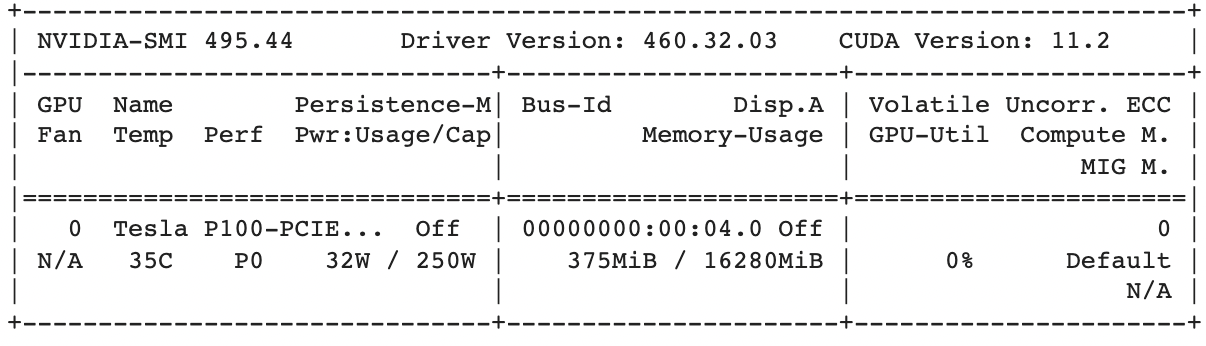
\includegraphics[width=1.0\linewidth]{img/nvidiagpu}
    \caption[Details of GPU]{GPU details}
    \label{fig:nvidiagpu}
\end{figure}
\begin{figure}[H]
    \centering
    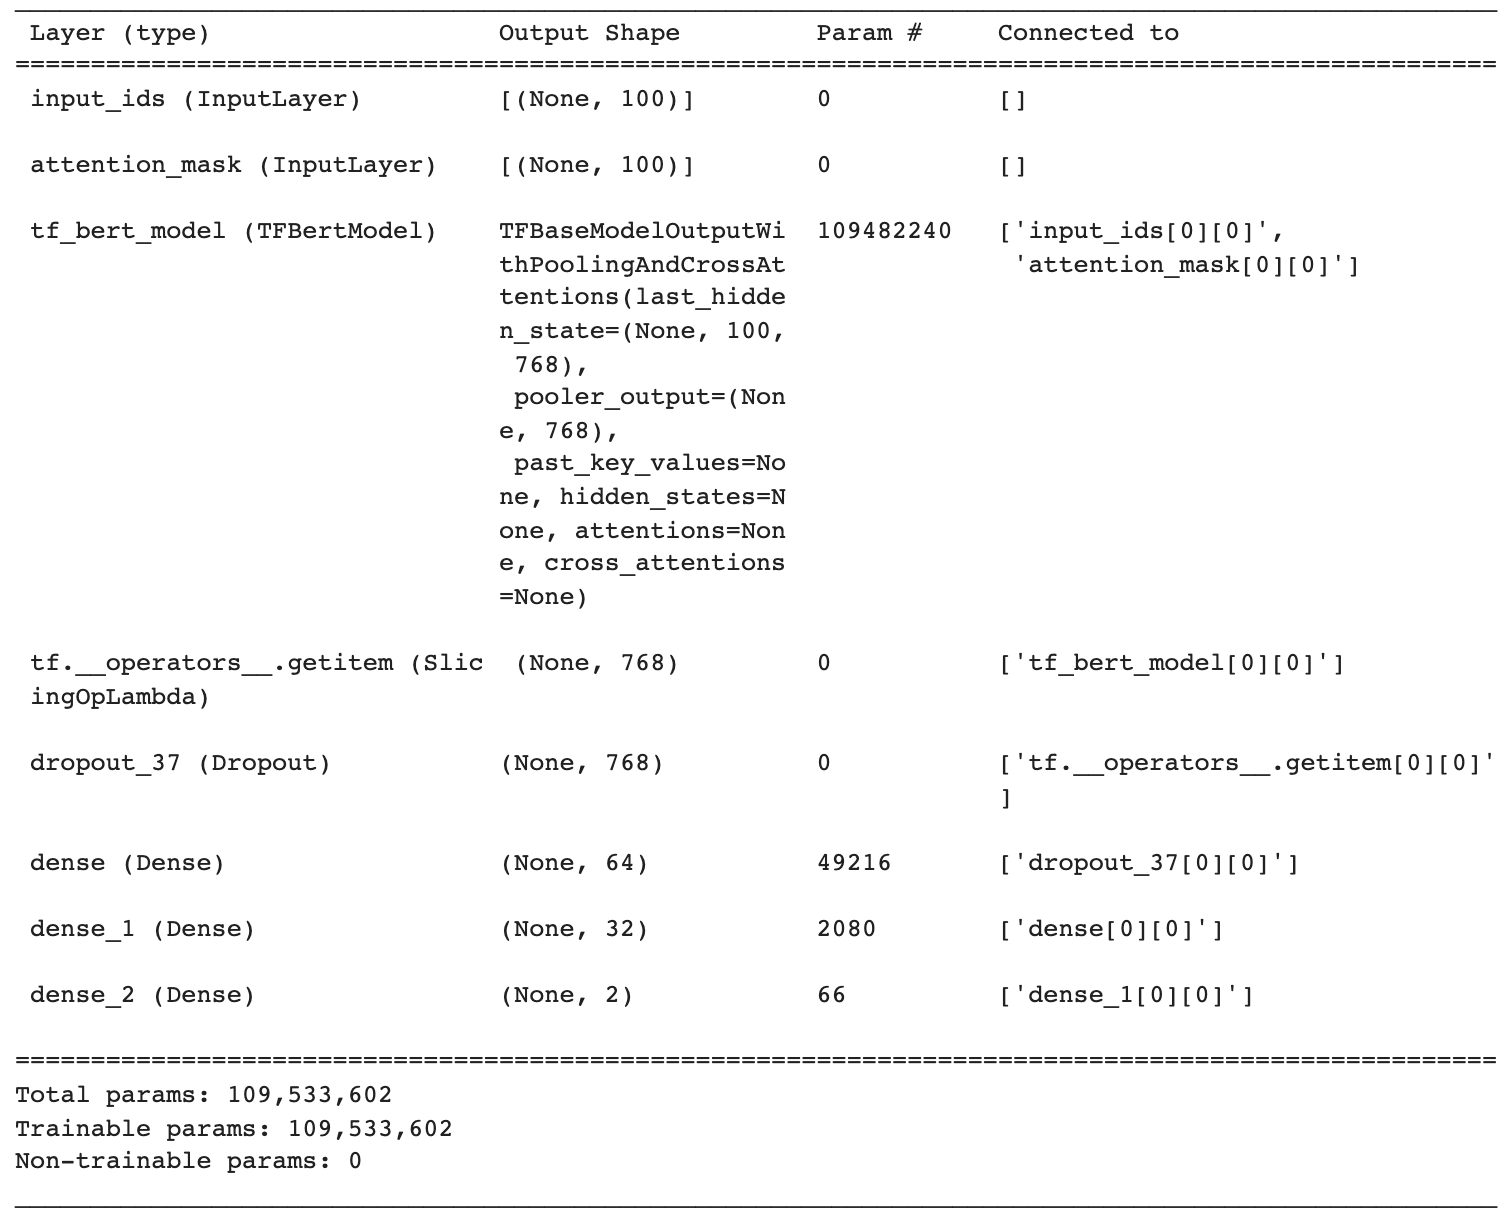
\includegraphics[width=0.9\linewidth]{img/bert_arch}
    \caption[ Layer diagram of BERT model used in the experiment]{Layer overview of BERT model used in experiment}
    \label{fig:bertarch}
\end{figure}
\begin{figure}[H]
    \centering
    \includegraphics[width=0.9\linewidth]{img/DistilBERTarch}
    \caption[Layer diagram of DistilBERT model used in the experiment]{Layer diagram of DistilBERT model used in the experiment}
    \label{fig:distilbertarch}
\end{figure}

\begin{figure}[H]
    \centering
%    \hspace*{2.5em}
    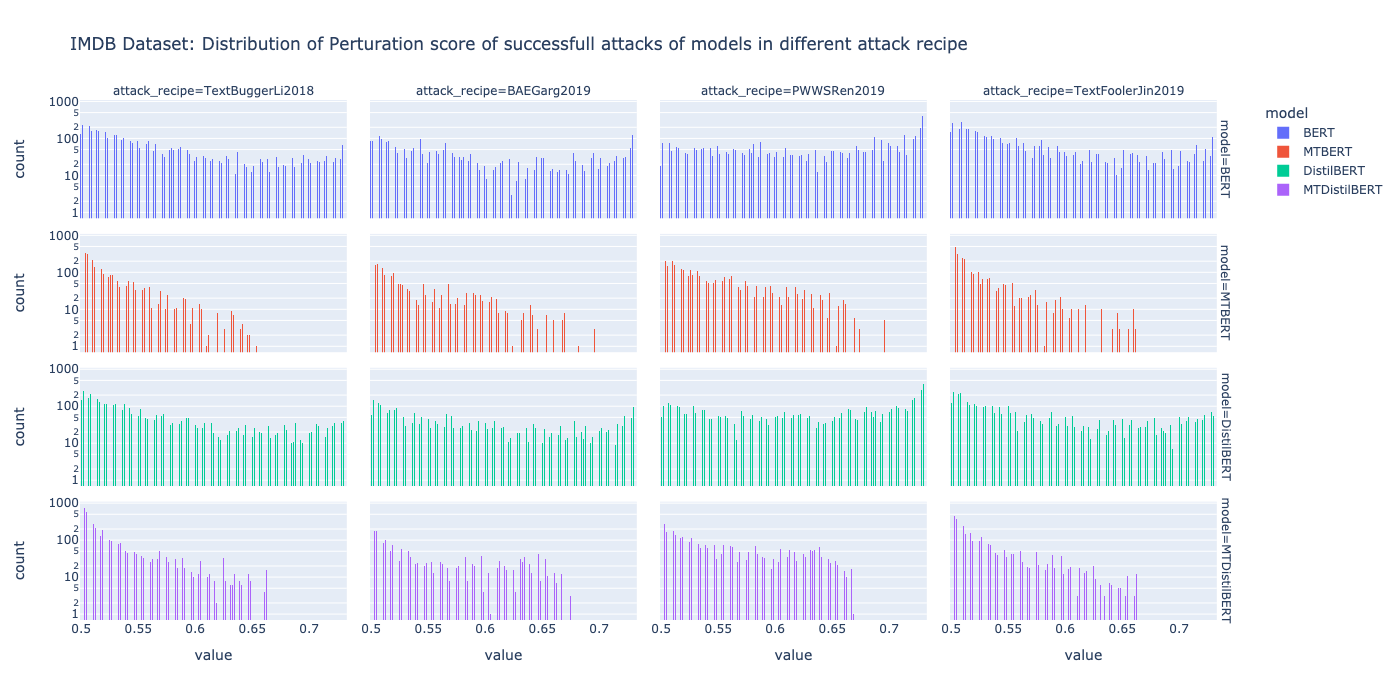
\includegraphics[width=1.1\linewidth]{img/PertScoreDist_IMDB.png}
    \caption[Distribution plot of perturbation score for IMDB Dataset]{Distribution plot of perturbation score for IMDB Dataset}
    \label{fig:PerturbationScore_Dist_IMDB}
\end{figure}
\begin{figure}[H]
    \centering
%    \hspace*{2.5em}
    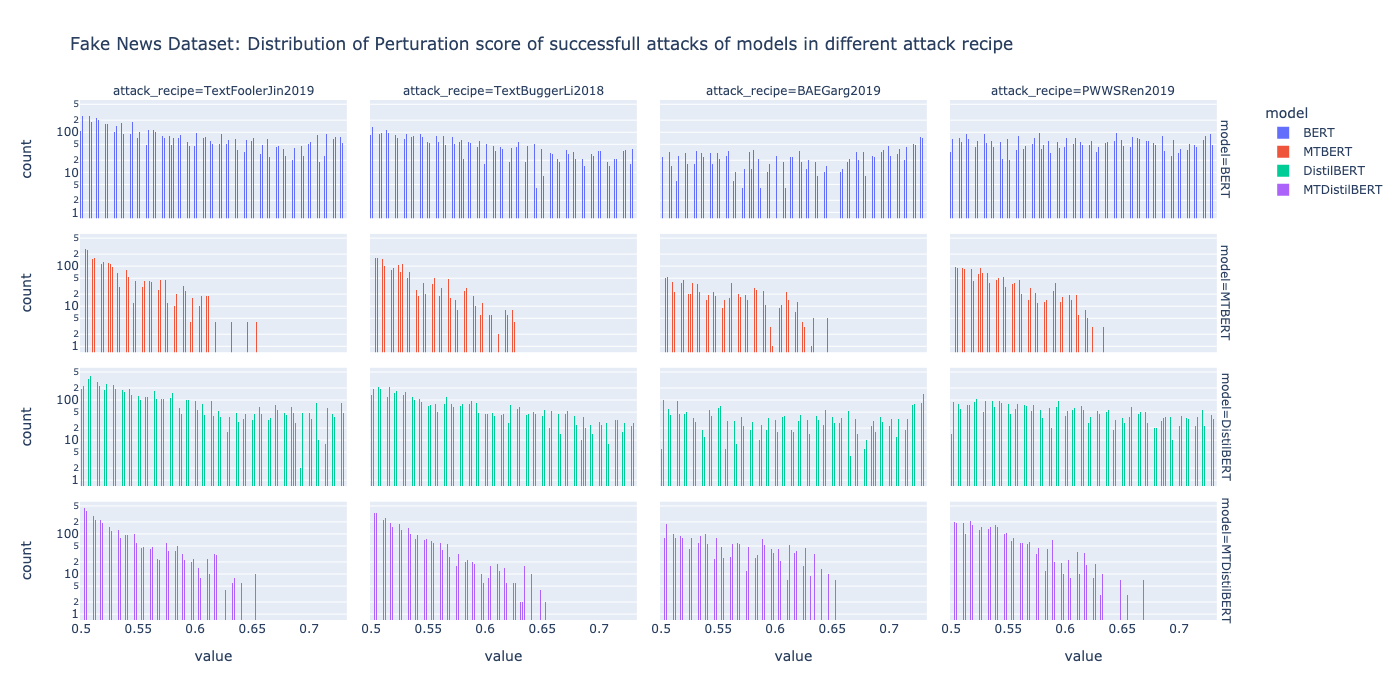
\includegraphics[width=1.1\linewidth]{img/PertScoreDist_fakenews.png}
    \caption[Distribution plot of perturbation score for Covid-19 fake tweets Dataset]{Distribution plot of perturbation score for Covid-19 fake tweets Dataset}
    \label{fig:PerturbationScore_Dist_fakenews}
\end{figure}
\begin{figure}[H]
    \centering
    %    \hspace*{2.5em}
    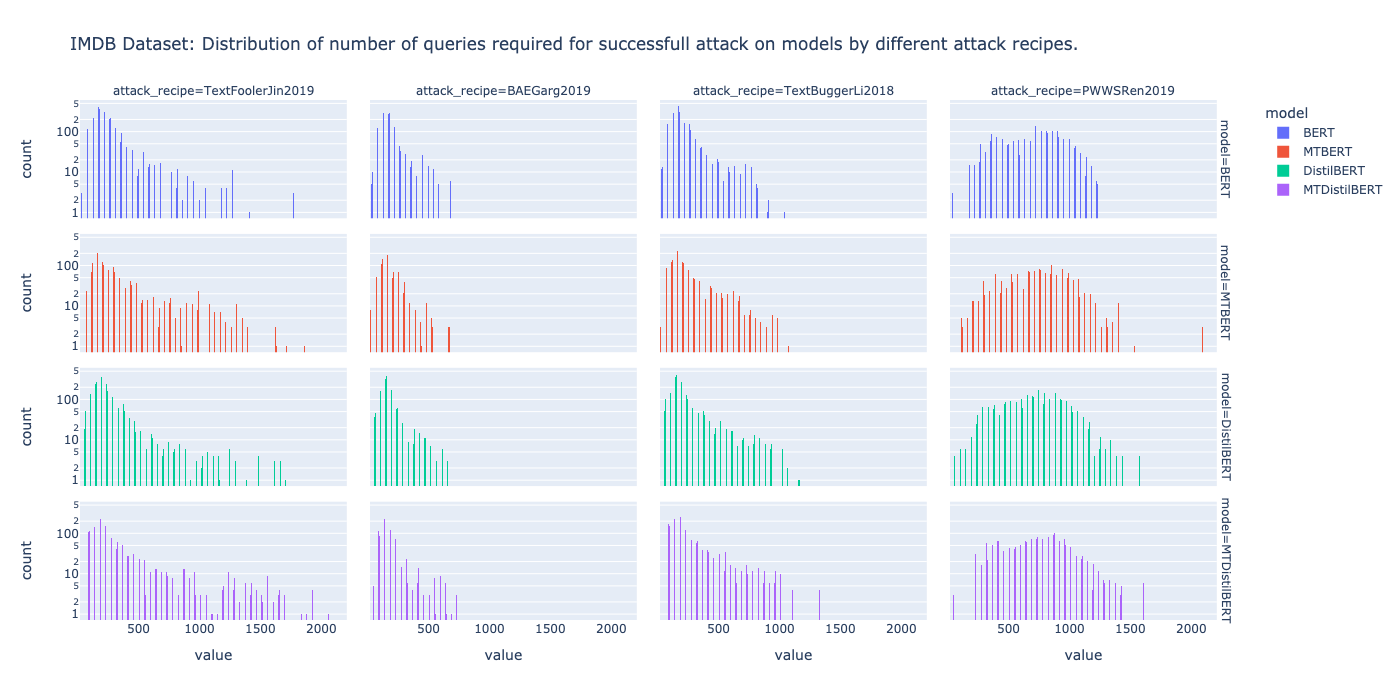
\includegraphics[width=1.1\linewidth]{img/NumQueriesDist_IMDB.png}
    \caption[Distribution plot of number of queries of IMDB Dataset]{Distribution plot of number of queries of  IMDB Dataset.}
    \label{fig:Queries_distribution_imdb}
\end{figure}
\begin{figure}[H]
    \centering
    %    \hspace*{2.5em}
    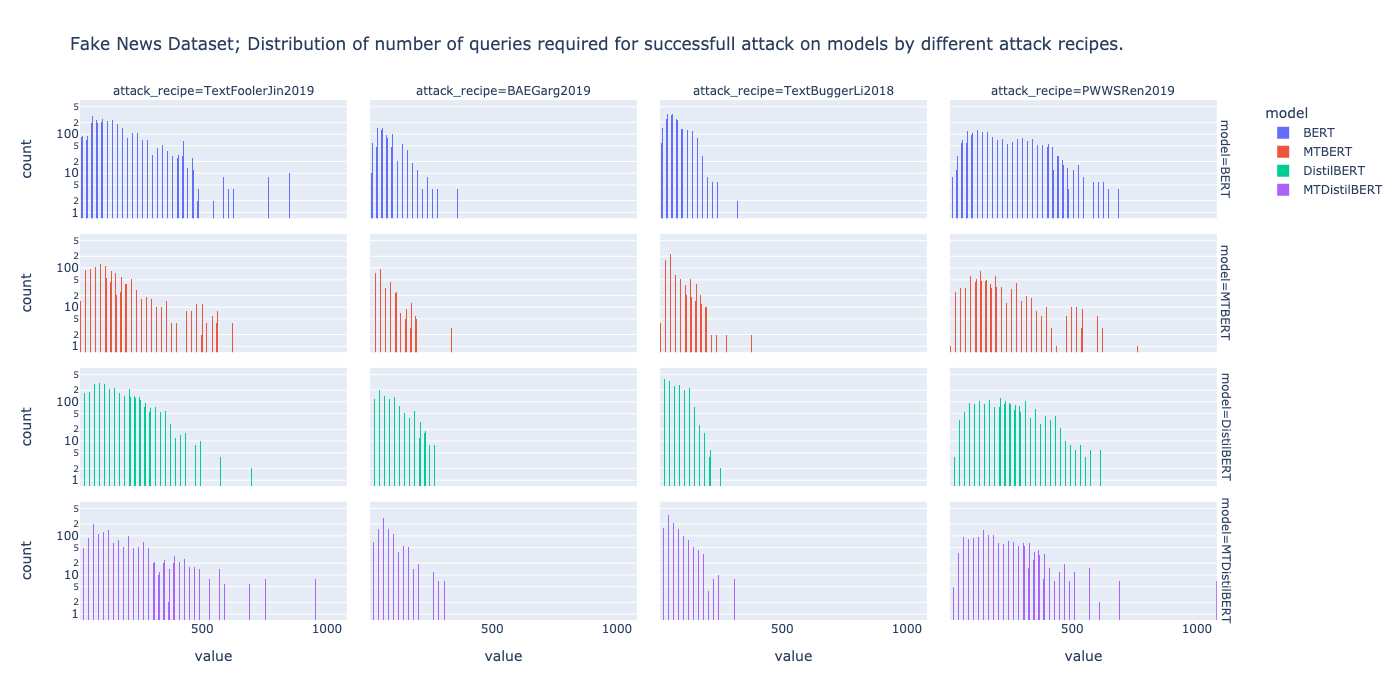
\includegraphics[width=1.1\linewidth]{img/NumQueriesDist_fknews.png}
    \caption[Distribution plot of number of queries of Covid-19 fake tweets Dataset]{Distribution plot of number of queries of Covid-19 fake tweets Dataset.}
    \label{fig:Queries_distribution_fk}
\end{figure}
\begin{figure}[H]
    \centering
    %    \hspace*{2.5em}
    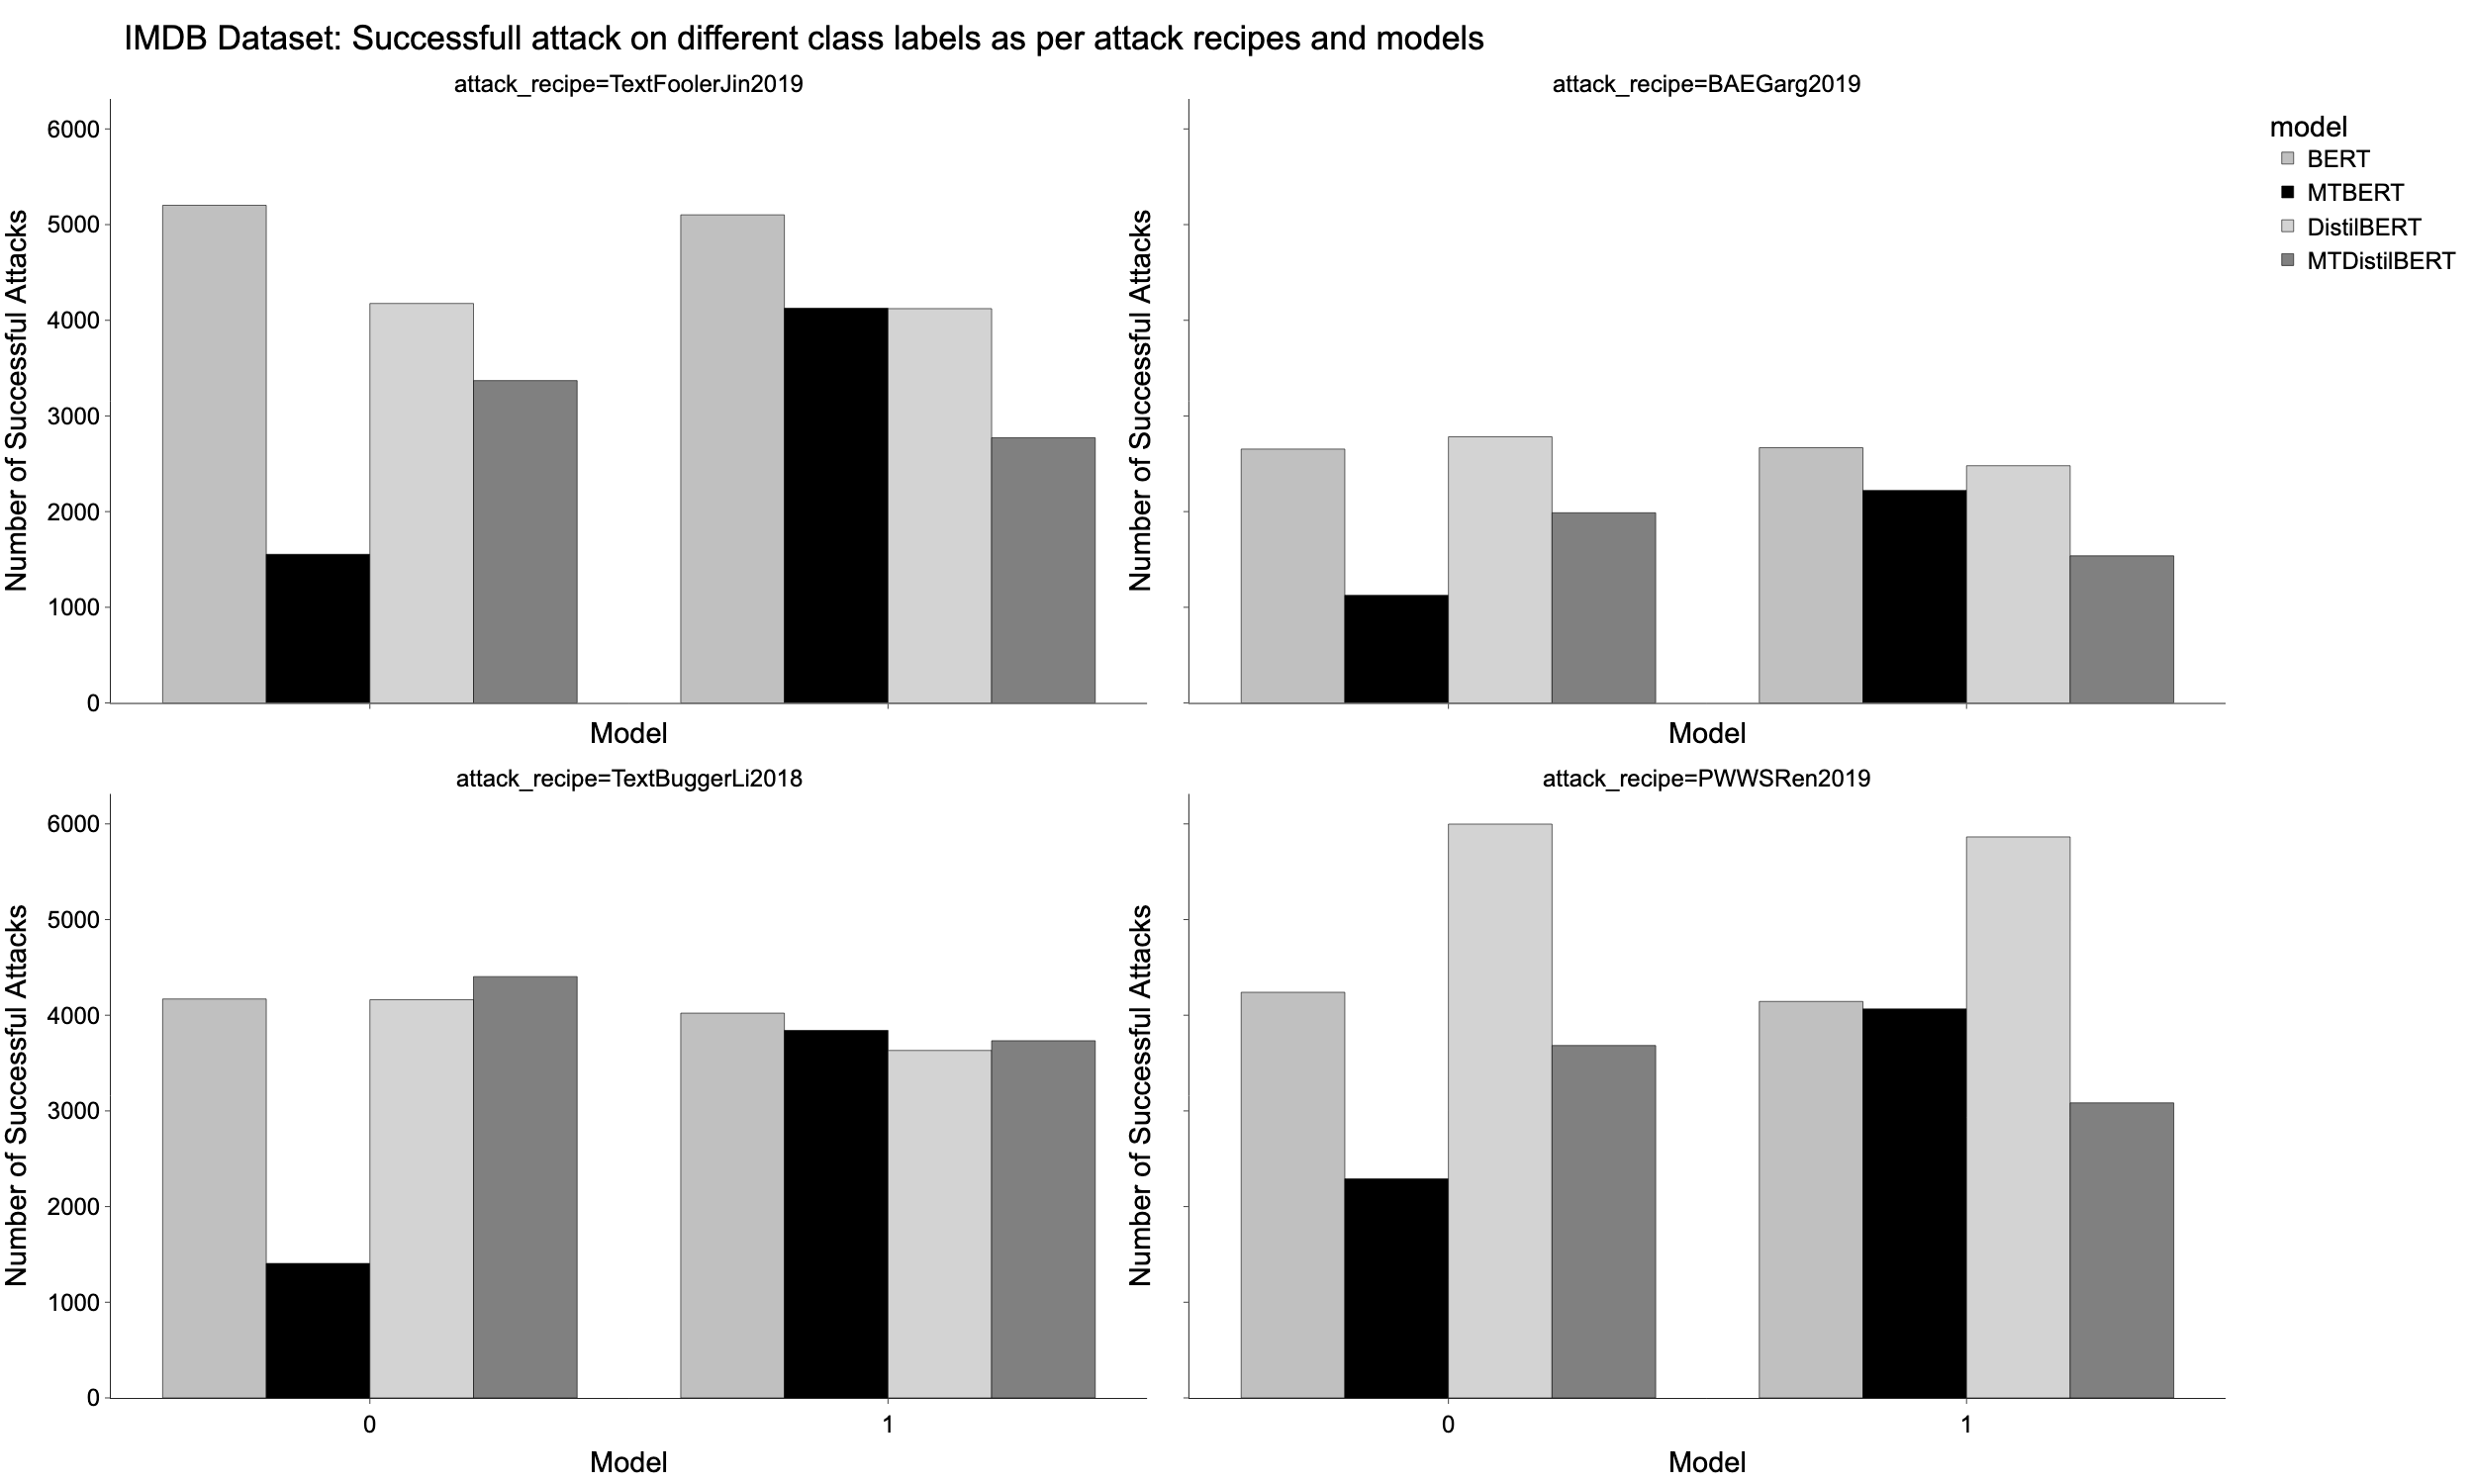
\includegraphics[width=1.0\linewidth]{img/IMDB_class_attack_1.png}
    \caption[Bar plot of successful attack on different class labels for IMDB dataset]{IMDB Dataset: Bar plot of successful attack on different class labels}
    \label{fig:classattack_imdb}
\end{figure}
\begin{figure}[H]
    \centering
    %    \hspace*{2.5em}
    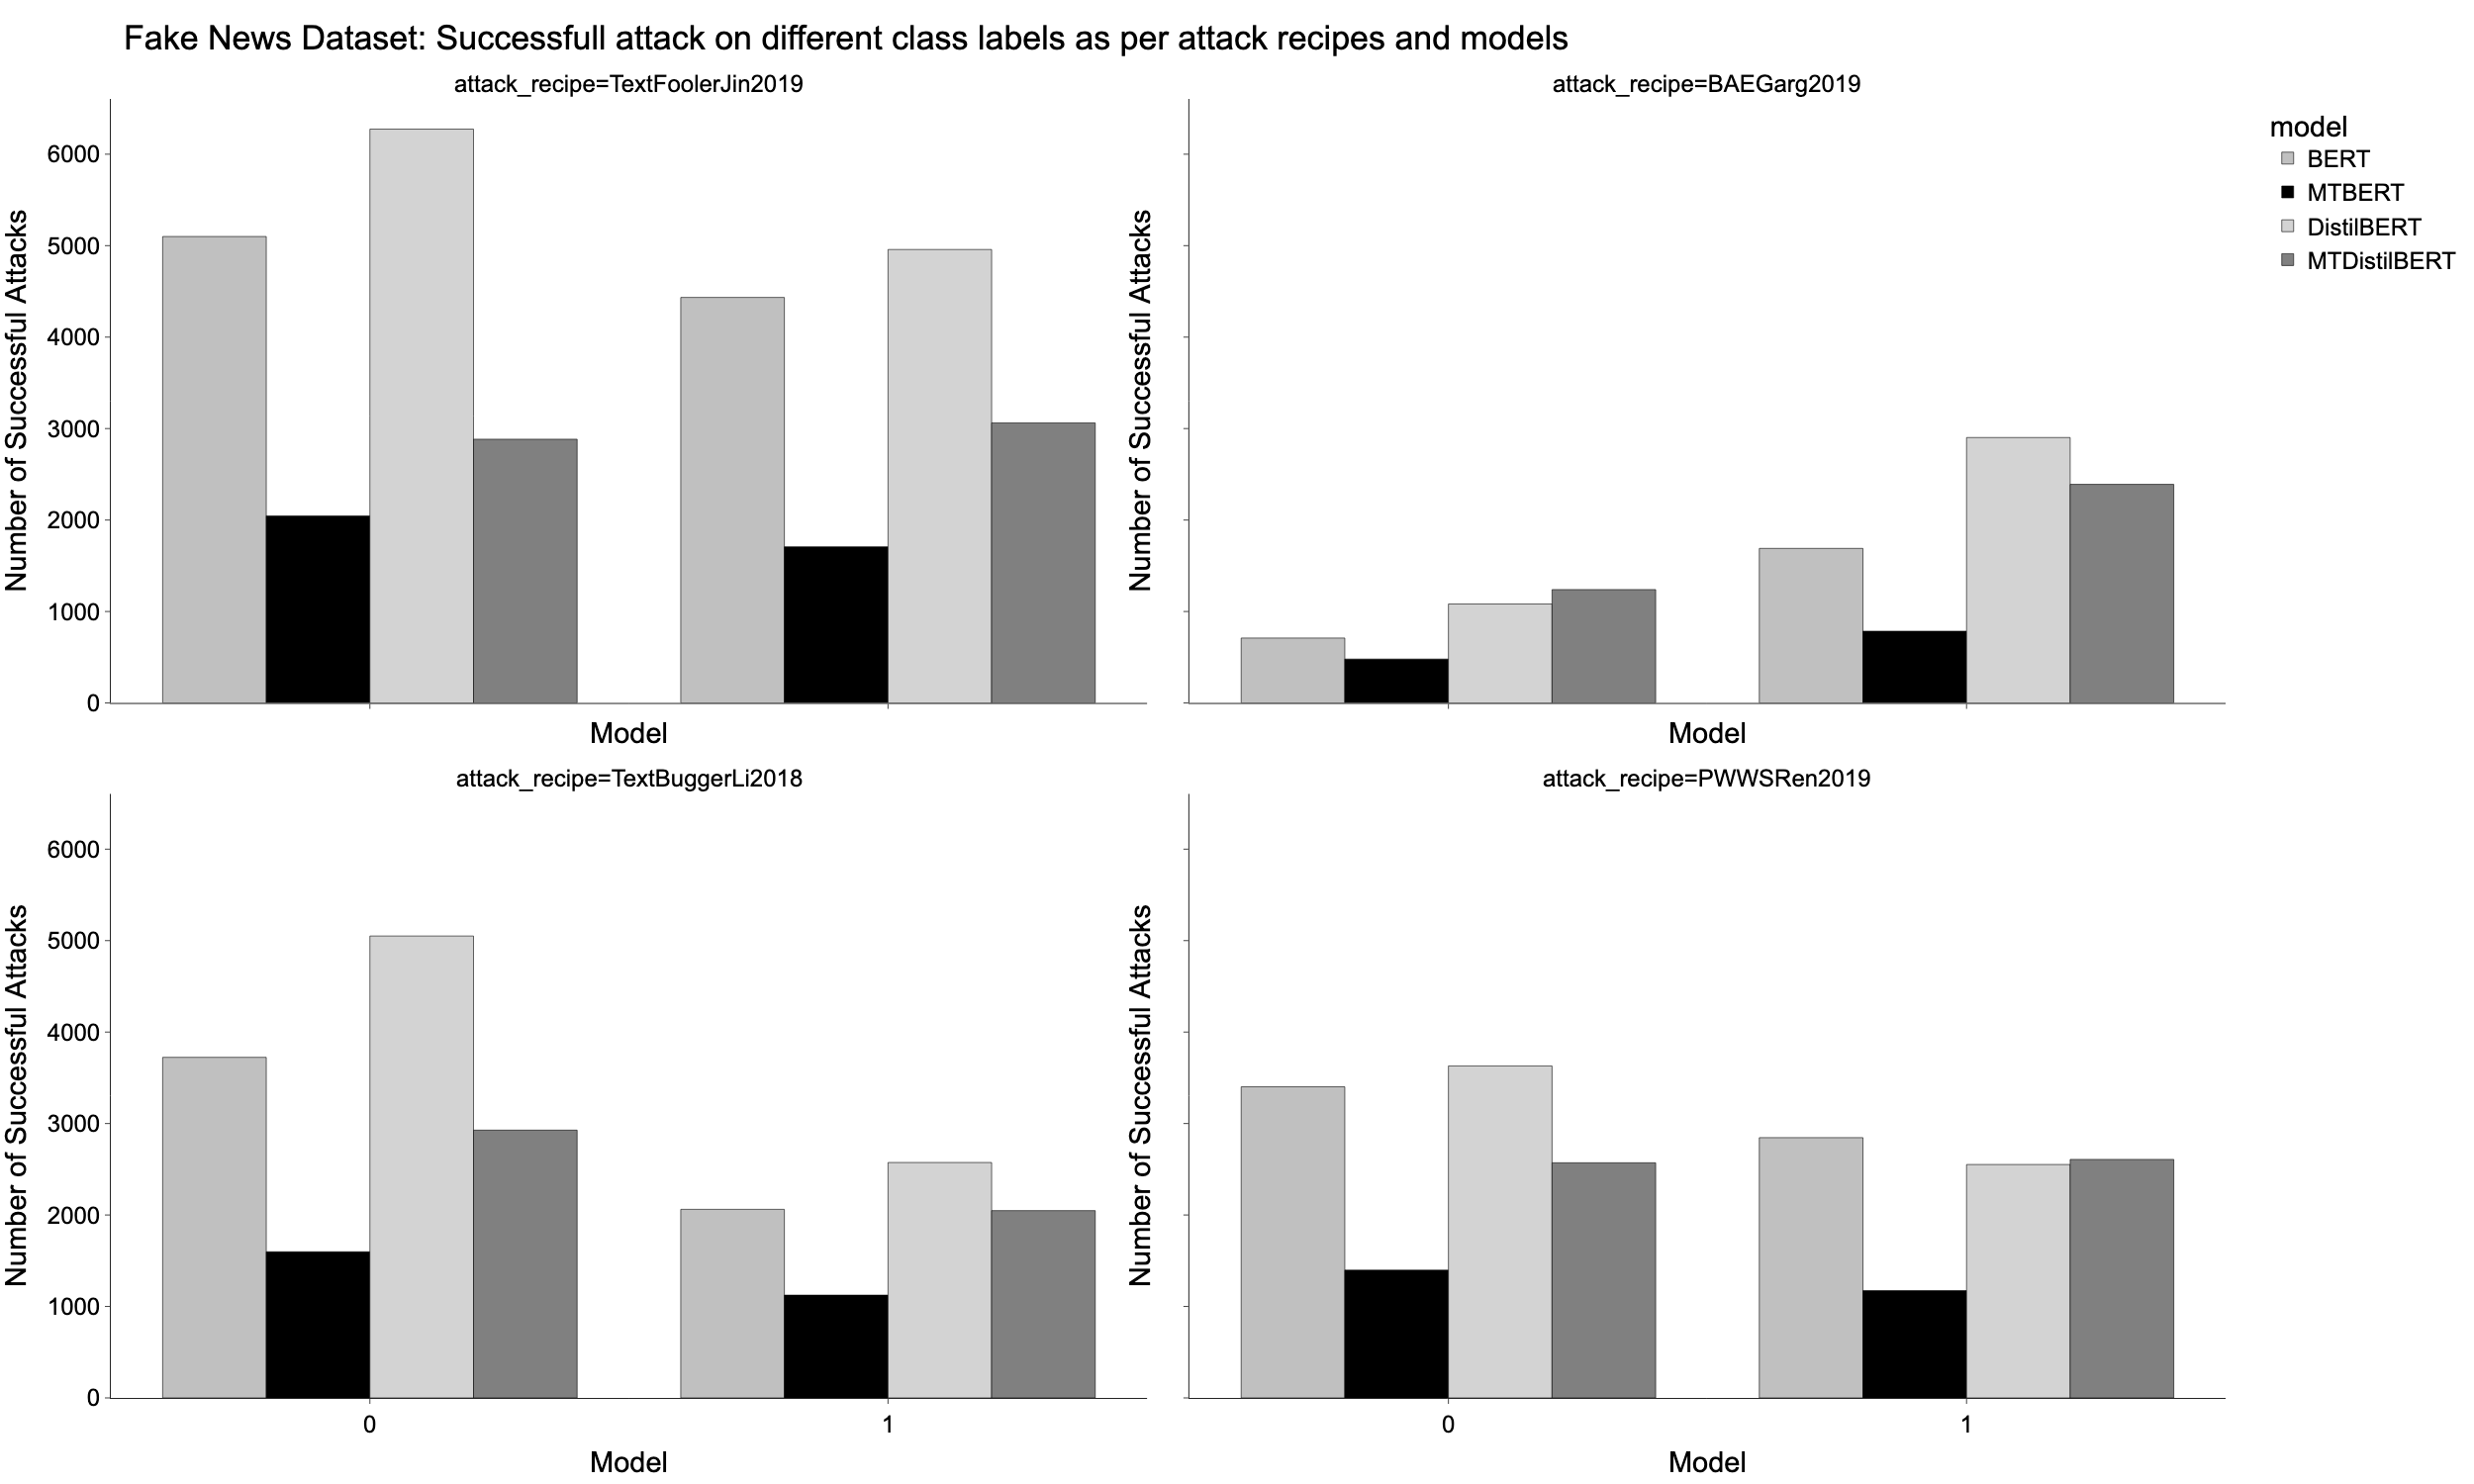
\includegraphics[width=1.0\linewidth]{img/fakenews_class_attack_1.png}
    \caption[Bar plot of successful attack on different class labels for Covid-19 fake tweets dataset]{Covid-19 fake tweets dataset: Bar plot of successful attack on different class labels }
    \label{fig:classattack_fakenews}
\end{figure}

\end{document}


% \section{.tex Organization}

% This folder contains the following base structure:

% \begin{figure}[h!]
% \centering
% \begin{forest}
%   for tree={
%     font=\sffamily,
%     grow'=0,
%     child anchor=west, % orientation
%     parent anchor=south,
%     anchor=west,
%     calign=first,
%     draw,
%     top color=white, %  colors
%     bottom color=blue!20,
%     edge+=->,
%     edge path={ % edge configuration
%       \noexpand\path [draw, \forestoption{edge}]
%       (!u.south west) +(7.5pt,0) |- node[fill,inner sep=1.25pt] {} (.child anchor)\forestoption{edge label};
%     },
%     before typesetting nodes={
%       if n=1
%         {insert before={[,phantom]}}
%         {}
%     },
%     l sep'+=10pt, % distances
%     s sep=15pt,
%     node options={inner sep=8pt},
%     fit=band,
%     before computing xy={l=15pt},
%   }
% [FG\_Mauthe\_latex\_template
%   [template.tex \textbf{(main document)}]
%   [bibThesis.bib]
%   [inc
%     [Titlepage.tex \textbf{(update!)}, bottom color=red!20]
%     [Declaration.tex]
%     [Abstract.tex \textbf{(update later!)}]
%     [Glossary.tex \textbf{(optional)}]
%   ]
%   [img
%     [uni-logo.png]
%     [iwvi.jpg]
%   ]
% ]
% \end{forest}

% \caption{Folder structure with contents of this thesis template.}\label{fig:tree}
% \end{figure}


% \textbf{Important}:

% \begin{enumerate}
% \item \textit{template.tex} is the main document.
% \item \textit{bibThesis.bib} contains your future references.
% \item The \textit{inc} folder contains the necessary \textit{.tex} documents to complete your thesis.

% \item \textbf{Before you proceed and delete this text and the dummy chapters, please be sure to replace every important field in the title page! See the folder \textit{inc} and file \textit{titlepage.tex}.} Then, you are free to start writing your thesis!

% \begin{enumerate}
% 	\item Replace the title.
% 	\item Decide if bachelor or master.
% 	\item Put your course of studies.
% 	\item Put your name and matriculation number.
% 	\item Put month and year of the submission of your thesis. Keep this in mind in case of possible changes.
% 	\item Choose the second referee ("Zweitgutachter").
% 	\item If there's a third person (i.e. external), uncomment the respective line in the \textit{titlepage.tex} file and list him or her as well.
% \end{enumerate}

% \item The glossary is optional and it is not included by default.
% \item Images, tables and diagrams belong to the \textit{img} folder, although you are free to add more folders to organize your work. Always add the folder as a prefix if you include an image, for instance, \texttt{\textbackslash includegraphics[width=200pt]\{\underline{img}/iwvi.jpg\}}

% \end{enumerate}

% \section{Recommendations}

% Here, we list some tips and notes.

% \begin{itemize}
% \item Every diagram / table / figure has a caption describing it. Diagram legends must be \textbf{effortlessly} readable.
% \item Every symbol, specifically math symbols, used throughout the text are to be described and properly introduced.
% \item Use present tense whenever possible.
% \item If you prefer a serif font, simply comment at the very beginning of the document \\\texttt{ \textbackslash renewcommand\{\textbackslash familydefault\}\{\textbackslash sfdefault\}}.
% \item If you would like to write your thesis in German, comment \texttt{\textbackslash usepackage[english]\{babel\}} and uncomment \texttt{\textbackslash usepackage[ngerman]\{babel\}} (at the very beginning of the document). For "Umlaute" use, for instance, the formula \textbackslash"o to write an \"o.
% \item If your thesis contains a lot of abbreviations, you can include a glossary. Uncomment the line right below the table of contents in the \textit{.tex} document. In the folder \textit{inc} you find the \textit{glossary.tex} file.
% \item For an appendix, you uncomment the package \texttt{\textbackslash usepackage[toc,page]\{appendix\}} and the given exemplary lines at the end of this \textit{.tex} document. \footnote[2]{Make very sparse use of footnotes}
% \end{itemize}


%===%

% \chapter{Short \LaTeX\ Guide}

% This chapter contains a very short list of rudimentary \LaTeX\ commands with explanations.


% \section{Including Graphics}

% Here, you see an example to include graphics.

% \begin{figure}[h]
% 	\centering
% 	
\includegraphics[width=200pt]{img/iwvi.jpg}
% 	\caption[IWVI Symbol]{This picture serves as an example in this template. It is the symbol of our institute. Always include a meaningful caption below a figure or table which explains the figure or table almost by itself. The text in the brackets [] next to \texttt{\textbackslash caption} appears in the table of figures.}
% 	 \label{fig:picLabel}
% \end{figure}

% With the \texttt{\textbackslash label\{labelName\}} command you can define a label and point to the reference with \texttt{\textbackslash ref\{labelName\}} in your text. Here is figure \ref{fig:picLabel} for example.


%===%

% \section{Including Equations}

% You can add equations, enumerate and reference them using \texttt{\textbackslash eqref}, like for equation \eqref{eq:error}.

% \begin{equation}
% \label{eq:error}
% \dfrac{\partial L}{\partial w_l} = (a_l - y_i) \sigma'(z_l) a_{l-1}
% \end{equation}

% If an equation consists of several parts, you can use \texttt{subequations} to number them.

% \begin{subequations}
% \begin{align}
% \mathbf{H}_1 &= 3 + 3 \\
% \mathbf{H}_2 &= 4 + 4  \\
% \mathbf{\hat Y} &= 5 + 5
% \end{align}
% \end{subequations}


%===%

% \section{Including Tables}

% The description given in the square brackets next to the \texttt{\textbackslash caption} command of table \ref{table:exampleTable} should appear in the list of tables. Additionally, \texttt{ \textbackslash multicolumn} and \texttt{ \textbackslash multirow} enables the combination of columns or rows.

% \begin{table}[th]
% \centering
% \begin{tabular}{ l c c }
% \hline
% Hyperparameter 		& \multicolumn{2}{c}{Used parameters in this work}\\
% \hline
% Optimizer 				& \multicolumn{2}{c}{Adam} \\
% Learning rate 			& \multicolumn{2}{c}{ $0.01$ } \\
% Loss function 			& \multicolumn{2}{c}{sparse categorical cross entropy}  \\
% Epochs 				& \multicolumn{2}{c}{$400$} \\
% Batch size 			& \multicolumn{2}{c}{32 } \\
% Dropout value 			& \multicolumn{2}{c}{0.1}  \\
% \midrule
% Results obtained in \%	& First run		& Second run \\
% \hline
% Accuracy 				& 0.955 		& 0.9522 \\
% Precision				& 0.955	 	& 0.952  \\
% Recall 				& 0.955  		& 0.952 \\
% F1-Score 				& 0.955		& 0.952
% \end{tabular}
% \caption[Hyperparameters with test run results]{This dummy table shows several hyperparameters used in two experiments with results of several metrics. }
% \label{table:exampleTable}
% \end{table}


%===%

% \chapter{Citing and References}

% Important information. \textbf{Please refer to our introduction to scientific writing ("Einf\"uhrung in das wissenschaftliche Schreiben") for further information as well}.

% \section{In General}

% How to cite correctly:

% \begin{itemize}
% \item \textcolor{red}{wrong}: ...as the related work indicates. \cite{Rose} \cite{ISLR} \cite{cuDNN} (\texttt{\textbackslash cite\{Rose\} \textbackslash cite\{ISLR\} \textbackslash cite\{cuDNN\}})
% \item \textcolor{blue}{correct}: ...as the related work indicates. \cite{Rose, ISLR, cuDNN} (\texttt{\textbackslash cite\{Rose, ISLR, cuDNN\}})
% \end{itemize}

%  \textbf{Don't reference sources you haven't read and don't omit references crucial to understand parts of your thesis. Keep in mind that this may be considered \underline{plagiarism} and your thesis is evaluated with \textit{not passed}, e.g., 5.0.}

% \section{Types of References}

% Here you find a list of different types of reference, ordered by importance respectively \textit{scientific} quality.

% \begin{enumerate}
% \item Journal articles, conference papers (good quality)
% \item Books
% \item Reports, tech reports, work reports
% \item Magazines
% \item Internet sources (exception is arXiv) (below average quality)
% \end{enumerate}

% \section{Must-Have Attributes}

% There are several must-have attributes certain reference types should always contain.

% \subsection{Article}

% See \cite{Rose} for an example.

% \begin{itemize}
% \item Title
% \item Names of the authors
% \item Year of publication
% \item Journal or source
% \end{itemize}

% \subsection{Book}

% See \cite{ISLR} for an example.

% \begin{itemize}
% \item Title
% \item Names of the authors
% \item Year of publication
% \item Publisher / Issuer
% \item Location
% \item If applicable, mention the page or chapter of the source, for instance \cite[p. 1]{ISLR} (\texttt{\textbackslash cite[p. 1]\{ISLR\}})or \cite[Chapter 1]{ISLR}
% \end{itemize}

% \subsection{Internet Source}

% See \cite{cuDNN} for an example.

% \begin{itemize}
% \item Title
% \item Names of the authors
% \item URL
% \item "Last accessed " + date
% \item Not mandatory but advisable to take a screenshot of a page! Websites may change or disappear.
% \end{itemize}

% Good luck with your thesis!




% Appendices if needed. There might be other ways to achieve this, like putting a separate .tex file in the inc folder
% even though this option presented would be valid, too.
%\begin{appendices}
%\chapter{Some Additional Information }
%Sample appendices chapter.
%\end{appendices}

%